% main.tex -- FrontierForge Phase 1 paper (revision 1, 1 October 2026; see RESPONSE.md for the changes).
%
% Venue-agnostic article layout. To move it into an arXiv, TMLR or workshop template, keep the body
% (\input{sections/...}), numbers.tex and the \ffdef / \val definitions below, and swap the preamble.
% Build:   latexmk -pdf main.tex      (from paper/; see README.md)
% Numbers: every data-derived number is \val{key}, defined in numbers.tex, which
%          paper/analysis/make_all.py regenerates from the repository's data. Do not type numbers by hand.
% Figures: every figure is generated at its printed width by paper/analysis (figures/*.pdf); place it at that width.
\documentclass[11pt]{article}

\usepackage[T1]{fontenc}
\usepackage{lmodern}
\usepackage[letterpaper,margin=1in]{geometry}   % text width 6.5 in = 469.75 pt; the figures are drawn for it
\usepackage{amsmath,amssymb}
\usepackage{booktabs}
\usepackage{array}
\usepackage{longtable}
\usepackage{graphicx}
\usepackage{xcolor}
\usepackage{microtype}
\usepackage{enumitem}
\usepackage[font=small,labelfont=bf]{caption}
\usepackage[round]{natbib}
\usepackage[colorlinks=true,linkcolor=blue!50!black,citecolor=blue!50!black,urlcolor=blue!50!black]{hyperref}
\usepackage[nameinlink]{cleveref}

\usepackage[section]{placeins}   % floats never drift past the end of their section

\graphicspath{{figures/}}
\setlist{nosep,leftmargin=*}
\setlength{\parskip}{0.25em}

% Float placement: let pages fill with floats rather than defer them.
\renewcommand{\topfraction}{0.9}
\renewcommand{\bottomfraction}{0.8}
\renewcommand{\textfraction}{0.07}
\renewcommand{\floatpagefraction}{0.75}
\setcounter{topnumber}{3}
\setcounter{bottomnumber}{2}
\setcounter{totalnumber}{5}

% ---------------------------------------------------------------- double-blind switch
% \anonymoustrue for MLSys / TMLR / other double-blind venues: hides the author block, the acknowledgements and
% the repository URL (the reproducibility statement then points to "an anonymised repository").
% \anonymousfalse (default) for arXiv and the camera-ready version.
\newif\ifanonymous
\anonymousfalse

% ---------------------------------------------------------------- generated numbers
% \ffdef{key}{value} stores a value; \val{key} prints it, or a loud ??key?? and a warning if it is undefined.
\newcommand{\ffdef}[2]{\expandafter\def\csname ffv@#1\endcsname{#2}}
\DeclareRobustCommand{\val}[1]{%
  \ifcsname ffv@#1\endcsname\csname ffv@#1\endcsname
  \else\textbf{??#1??}\PackageWarning{ffnumbers}{Undefined value `#1'}\fi}
% numbers.tex -- GENERATED by paper/analysis/make_all.py; do not edit by hand.
% Each value: \ffdef{key}{value}; used in the text as \val{key}. The comment names the source.

\ffdef{n-scored}{34}  % results/official-scores.csv
\ffdef{n-rehearsed}{30}  % results/official-scores.csv
\ffdef{n-official-tests}{4}  % results/official-scores.csv
\ffdef{first-official}{1.1463}  % results/official-scores.csv
\ffdef{first-name}{F2}  % results/official-scores.csv
\ffdef{best-official}{0.96136}  % results/official-scores.csv
\ffdef{best-official-long}{0.9613617}  % results/official-scores.csv
\ffdef{best-name}{K82s4}  % results/official-scores.csv
\ffdef{best-rehearsal}{0.954472}  % results/official-scores.csv
\ffdef{best-steps}{2{,}388}  % results/official-scores.csv
\ffdef{kfortyfour-official}{0.9888}  % results/official-scores.csv
\ffdef{salt7-official}{0.96140}  % results/official-scores.csv
\ffdef{salt7-official-long}{0.9613955}  % results/official-scores.csv
\ffdef{salt7-rehearsal}{0.954379}  % results/official-scores.csv
\ffdef{salt7-steps}{2{,}405}  % results/official-scores.csv
\ffdef{descent-total}{0.1849}  % results/official-scores.csv
\ffdef{descent-from-kfortyfour}{0.0274}  % results/official-scores.csv
\ffdef{steps-ktwentyfour}{912}  % results/official-scores.csv
\ffdef{steps-ratio-best-ktwentyfour}{2.62}  % results/official-scores.csv
\ffdef{off-n-chipc}{7}  % results/official-scores.csv
\ffdef{off-mean-chipc}{\ensuremath{+}0.00653}  % results/official-scores.csv
\ffdef{off-mean-chipc-short}{\ensuremath{+}0.0065}  % results/official-scores.csv
\ffdef{off-sd-chipc}{0.00042}  % results/official-scores.csv
\ffdef{off-sd-chipc-short}{0.0004}  % results/official-scores.csv
\ffdef{off-min-chipc}{\ensuremath{+}0.0061}  % results/official-scores.csv (half-up)
\ffdef{off-max-chipc}{\ensuremath{+}0.0072}  % results/official-scores.csv (half-up)
\ffdef{off-ci-chipc}{0.00039}  % results/official-scores.csv
\ffdef{off-n-final}{7}  % results/official-scores.csv
\ffdef{off-mean-final}{\ensuremath{+}0.00687}  % results/official-scores.csv
\ffdef{off-mean-final-short}{\ensuremath{+}0.0069}  % results/official-scores.csv
\ffdef{off-sd-final}{0.00030}  % results/official-scores.csv
\ffdef{off-sd-final-short}{0.0003}  % results/official-scores.csv
\ffdef{off-min-final}{\ensuremath{+}0.0065}  % results/official-scores.csv (half-up)
\ffdef{off-max-final}{\ensuremath{+}0.0074}  % results/official-scores.csv (half-up)
\ffdef{off-ci-final}{0.00027}  % results/official-scores.csv
\ffdef{off-n-since}{15}  % results/official-scores.csv
\ffdef{off-mean-since}{\ensuremath{+}0.00671}  % results/official-scores.csv
\ffdef{off-mean-since-short}{\ensuremath{+}0.0067}  % results/official-scores.csv
\ffdef{off-sd-since}{0.00038}  % results/official-scores.csv
\ffdef{off-sd-since-short}{0.0004}  % results/official-scores.csv
\ffdef{off-min-since}{\ensuremath{+}0.0061}  % results/official-scores.csv (half-up)
\ffdef{off-max-since}{\ensuremath{+}0.0074}  % results/official-scores.csv (half-up)
\ffdef{off-ci-since}{0.00021}  % results/official-scores.csv
\ffdef{off-n-early}{15}  % results/official-scores.csv
\ffdef{off-mean-early}{\ensuremath{+}0.00626}  % results/official-scores.csv
\ffdef{off-mean-early-short}{\ensuremath{+}0.0063}  % results/official-scores.csv
\ffdef{off-sd-early}{0.00072}  % results/official-scores.csv
\ffdef{off-sd-early-short}{0.0007}  % results/official-scores.csv
\ffdef{off-min-early}{\ensuremath{+}0.0053}  % results/official-scores.csv (half-up)
\ffdef{off-max-early}{\ensuremath{+}0.0078}  % results/official-scores.csv (half-up)
\ffdef{off-ci-early}{0.00040}  % results/official-scores.csv
\ffdef{off-n-all}{30}  % results/official-scores.csv
\ffdef{off-mean-all}{\ensuremath{+}0.00648}  % results/official-scores.csv
\ffdef{off-mean-all-short}{\ensuremath{+}0.0065}  % results/official-scores.csv
\ffdef{off-sd-all}{0.00061}  % results/official-scores.csv
\ffdef{off-sd-all-short}{0.0006}  % results/official-scores.csv
\ffdef{off-min-all}{\ensuremath{+}0.0053}  % results/official-scores.csv (half-up)
\ffdef{off-max-all}{\ensuremath{+}0.0078}  % results/official-scores.csv (half-up)
\ffdef{off-ci-all}{0.00023}  % results/official-scores.csv
\ffdef{chip-off-b}{\ensuremath{+}0.00686}  % results/official-scores.csv
\ffdef{chip-off-n-b}{1}  % results/official-scores.csv
\ffdef{chip-off-c}{\ensuremath{+}0.00652}  % results/official-scores.csv
\ffdef{chip-off-n-c}{8}  % results/official-scores.csv
\ffdef{chip-ferr-c}{\ensuremath{-}0.00004}  % results/official-scores.csv: frozen chip-C error, mean by chip
\ffdef{chip-off-e}{\ensuremath{+}0.00655}  % results/official-scores.csv
\ffdef{chip-off-n-e}{1}  % results/official-scores.csv
\ffdef{chip-ferr-e}{\ensuremath{+}0.00003}  % results/official-scores.csv: frozen chip-C error, mean by chip
\ffdef{chip-off-h}{\ensuremath{+}0.00684}  % results/official-scores.csv
\ffdef{chip-off-n-h}{2}  % results/official-scores.csv
\ffdef{chip-ferr-h}{\ensuremath{+}0.00031}  % results/official-scores.csv: frozen chip-C error, mean by chip
\ffdef{chip-off-g}{\ensuremath{+}0.00712}  % results/official-scores.csv
\ffdef{chip-off-n-g}{3}  % results/official-scores.csv
\ffdef{chip-ferr-g}{\ensuremath{+}0.00059}  % results/official-scores.csv: frozen chip-C error, mean by chip
\ffdef{off-sd-within}{0.00034}  % results/official-scores.csv: pooled within-chip SD since K50
\ffdef{off-sd-within-lo}{0.00024}  % results/official-scores.csv: chi-square 95% CI of the pooled within-chip SD, 10 df
\ffdef{off-sd-within-hi}{0.00059}  % results/official-scores.csv
\ffdef{loo-n}{13}  % results/official-scores.csv
\ffdef{loo-pooled-mae}{0.00036}  % results/official-scores.csv: leave-one-out, pooled mean
\ffdef{loo-chip-mae}{0.00028}  % results/official-scores.csv: leave-one-out, same-chip mean
\ffdef{diff-sd}{0.00053}  % sqrt(2) x since-K50 offset SD
\ffdef{diff-95}{0.0010}  % 1.96 sqrt(2) x since-K50 offset SD
\ffdef{diff-sd-within}{0.00048}  % sqrt(2) x within-chip offset SD
\ffdef{diff-95-within}{0.0009}  % 1.96 sqrt(2) x within-chip offset SD
\ffdef{pi-half}{0.0008}  % 95% prediction half-width at n=15
\ffdef{gap-n}{18}  % research/sim-data/runs.jsonl: bpb_20m - bpb_2m
\ffdef{gap-chips}{C}  % research/sim-data/runs.jsonl: bpb_20m - bpb_2m: chips of those runs
\ffdef{gap-mean}{\ensuremath{+}0.00712}  % research/sim-data/runs.jsonl: bpb_20m - bpb_2m
\ffdef{gap-sd}{0.00012}  % research/sim-data/runs.jsonl: bpb_20m - bpb_2m
\ffdef{gap-min}{\ensuremath{+}0.00696}  % research/sim-data/runs.jsonl: bpb_20m - bpb_2m
\ffdef{gap-max}{\ensuremath{+}0.00739}  % research/sim-data/runs.jsonl: bpb_20m - bpb_2m
\ffdef{gap-order-k}{146}  % research/sim-data/runs.jsonl: bpb_20m - bpb_2m: run pairs ordered the same on both texts
\ffdef{gap-order-pairs}{153}  % research/sim-data/runs.jsonl: bpb_20m - bpb_2m
\ffdef{gap-order-agree}{95\%}  % research/sim-data/runs.jsonl: bpb_20m - bpb_2m: share of run pairs ordered the same
\ffdef{gap-r}{0.995}  % research/sim-data/runs.jsonl: bpb_20m - bpb_2m: Pearson r between the two scores
\ffdef{offdec-round}{0.00003}  % SD of rounding to 4 decimals, 0.0001/sqrt(12)
\ffdef{offdec-text}{0.00012}  % research/sim-data/runs.jsonl: SD of bpb_20m - bpb_2m (= gap-sd)
\ffdef{offdec-rest}{0.00031}  % sqrt(within-chip SD^2 - text-gap SD^2 - rounding SD^2)
\ffdef{offdec-rest-lo}{0.00020}  % remainder at the lower chi-square limit of the within-chip SD
\ffdef{offdec-rest-hi}{0.00058}  % remainder at the upper chi-square limit of the within-chip SD
\ffdef{offdec-text-share}{13\%}  % text-gap variance as a share of the within-chip offset variance
\ffdef{offdec-rest-share}{87\%}  % remainder variance as a share of the within-chip offset variance
\ffdef{frozen-offset}{\ensuremath{+}0.00653}  % results/official-scores.csv
\ffdef{ferr-k82s4}{\ensuremath{+}0.00036}  % results/official-scores.csv: frozen chip-C error
\ffdef{ferr-k82s7}{\ensuremath{+}0.00049}  % results/official-scores.csv: frozen chip-C error
\ffdef{t-two}{4.3}  % Student t quantile, 2 df
\ffdef{holdout-n}{7}  % results/official-scores.csv
\ffdef{holdout-mae}{0.00035}  % results/official-scores.csv
\ffdef{holdout-bias}{\ensuremath{+}0.00034}  % results/official-scores.csv
\ffdef{holdout-maxerr}{0.00083}  % results/official-scores.csv
\ffdef{holdout-mae-lo}{0.00017}  % results/official-scores.csv: percentile bootstrap over the final-day uploads, 4000 draws, rng 0
\ffdef{holdout-mae-hi}{0.00055}  % results/official-scores.csv: percentile bootstrap
\ffdef{holdout-npos}{6}  % results/official-scores.csv
\ffdef{holdout-signp}{0.06}  % one-sided sign test, Binomial(n, 1/2)
\ffdef{holdout-mae-direct}{0.00053}  % results/official-scores.csv
\ffdef{holdout-n-direct}{3}  % results/official-scores.csv
\ffdef{holdout-mae-inherited}{0.00040}  % results/official-scores.csv
\ffdef{holdout-n-inherited}{2}  % results/official-scores.csv
\ffdef{holdout-mae-none}{0.00003}  % results/official-scores.csv
\ffdef{holdout-n-none}{2}  % results/official-scores.csv
\ffdef{seq-n}{12}  % results/official-scores.csv
\ffdef{seq-mae}{0.00031}  % results/official-scores.csv
\ffdef{seq-bias}{\ensuremath{+}0.00018}  % results/official-scores.csv
\ffdef{seq-inside}{12}  % results/official-scores.csv
\ffdef{seq-maxerr}{0.00083}  % results/official-scores.csv
\ffdef{seq-first}{K54b}  % results/official-scores.csv
\ffdef{seq-expected}{11.4}  % 0.95 x n
\ffdef{nooffset-mae}{0.0069}  % results/official-scores.csv: final-day uploads, offset 0
\ffdef{nooffset-mae-since}{0.0067}  % results/official-scores.csv: uploads since K50, offset 0
\ffdef{priormean-mae}{0.00050}  % results/official-scores.csv: final day, predicted by the mean of every earlier rehearsed upload
\ffdef{priormean-n}{23}  % results/official-scores.csv
\ffdef{priormean-offset}{\ensuremath{+}0.00637}  % results/official-scores.csv
\ffdef{priorsince-mae}{0.00033}  % results/official-scores.csv: final day, predicted by the mean of the earlier uploads since K50
\ffdef{priorsince-n}{8}  % results/official-scores.csv
\ffdef{earlymean-mae}{0.00061}  % results/official-scores.csv: final day, predicted by the mean of the early uploads (chips A/B, F2-K46)
\ffdef{earlymean-n}{15}  % results/official-scores.csv
\ffdef{earlymean-offset}{\ensuremath{+}0.00626}  % results/official-scores.csv
\ffdef{conc-n}{105}  % results/official-scores.csv: pairs of uploads since K50
\ffdef{conc-agree}{102}  % results/official-scores.csv: pairs ordered the same by rehearsal and official score
\ffdef{conc-ties}{1}  % results/official-scores.csv: pairs with equal official scores
\ffdef{conc-disagree}{2}  % results/official-scores.csv
\ffdef{conc-close-thr}{0.0005}  % rehearsal difference below which a pair counts as close
\ffdef{conc-close-n}{6}  % results/official-scores.csv: pairs whose rehearsals differ by less than 0.0005
\ffdef{conc-close-agree}{4}  % results/official-scores.csv
\ffdef{cq-n}{15}  % results/official-scores.csv, uploads since K50
\ffdef{cq-gh-n}{5}  % results/official-scores.csv, uploads since K50: uploads rehearsed on instances G and H
\ffdef{cq-slope}{\ensuremath{-}0.029}  % results/official-scores.csv, uploads since K50: d offset / d rehearsal bpb, no instance term
\ffdef{cq-slope-lo}{\ensuremath{-}0.070}  % results/official-scores.csv, uploads since K50: 95% t interval
\ffdef{cq-slope-hi}{\ensuremath{+}0.013}  % results/official-scores.csv, uploads since K50
\ffdef{cq-slope-p}{0.16}  % results/official-scores.csv, uploads since K50: two-sided t test of the slope
\ffdef{cq-slope-span}{0.00042}  % results/official-scores.csv, uploads since K50: |slope| x the since-K50 rehearsal span
\ffdef{cq-slope-adj}{\ensuremath{+}0.008}  % results/official-scores.csv, uploads since K50: slope with a G/H indicator
\ffdef{cq-slope-adj-lo}{\ensuremath{-}0.050}  % results/official-scores.csv, uploads since K50
\ffdef{cq-slope-adj-hi}{\ensuremath{+}0.066}  % results/official-scores.csv, uploads since K50
\ffdef{cq-gh-coef}{\ensuremath{+}0.00051}  % results/official-scores.csv, uploads since K50: G/H indicator, given the rehearsal score
\ffdef{cq-gh-lo}{\ensuremath{-}0.00008}  % results/official-scores.csv, uploads since K50: 95% t interval
\ffdef{cq-gh-hi}{\ensuremath{+}0.00110}  % results/official-scores.csv, uploads since K50
\ffdef{cq-gh-diff}{\ensuremath{+}0.00045}  % results/official-scores.csv, uploads since K50: mean offset, G/H minus the rest
\ffdef{cq-perm-n}{3{,}003}  % results/official-scores.csv, uploads since K50: label assignments enumerated
\ffdef{cq-perm-p}{0.026}  % results/official-scores.csv, uploads since K50: exact two-sided permutation p, G/H mean difference
\ffdef{cq-perm-p-adj}{0.087}  % results/official-scores.csv, uploads since K50: exact two-sided permutation p, G/H coefficient given the rehearsal score
\ffdef{k70a-raw}{0.957259}  % results/official-scores.csv (note column)
\ffdef{k70a-norm}{0.955946}  % results/official-scores.csv
\ffdef{k70a-adj}{0.00131}  % results/official-scores.csv: raw - normalised
\ffdef{k70a-adj-pct}{2.3\%}  % adjustment expressed in % steps at 0.00057 per 1%
\ffdef{k70a-raw-offset}{\ensuremath{+}0.0052}  % results/official-scores.csv
\ffdef{sens-used-sd}{0.00038}  % results/official-scores.csv
\ffdef{sens-used-mae}{0.00035}  % results/official-scores.csv
\ffdef{sens-used-inside}{12/12}  % results/official-scores.csv
\ffdef{sens-used-k70a-err}{\ensuremath{+}0.03}  % results/official-scores.csv
\ffdef{sens-raw-sd}{0.00054}  % results/official-scores.csv
\ffdef{sens-raw-mae}{0.00053}  % results/official-scores.csv
\ffdef{sens-raw-inside}{11/12}  % results/official-scores.csv
\ffdef{sens-raw-k70a-err}{\ensuremath{-}1.29}  % results/official-scores.csv
\ffdef{sens-excl-sd}{0.00039}  % results/official-scores.csv
\ffdef{sens-excl-mae}{0.00040}  % results/official-scores.csv
\ffdef{sens-excl-inside}{11/11}  % results/official-scores.csv
\ffdef{cov-50-b3}{7/12}  % results/official-scores.csv
\ffdef{cov-50-b5}{6/10}  % results/official-scores.csv
\ffdef{cov-80-b3}{11/12}  % results/official-scores.csv
\ffdef{cov-80-b5}{9/10}  % results/official-scores.csv
\ffdef{cov-95-b3}{12/12}  % results/official-scores.csv
\ffdef{cov-95-b5}{10/10}  % results/official-scores.csv
\ffdef{reg-slope}{0.971}  % results/official-scores.csv
\ffdef{reg-lo}{0.930}  % results/official-scores.csv
\ffdef{reg-hi}{1.013}  % results/official-scores.csv
\ffdef{reg-r}{0.9974}  % results/official-scores.csv
\ffdef{trend-slope}{\ensuremath{+}3.42}  % results/official-scores.csv
\ffdef{trend-lo}{\ensuremath{-}1.21}  % results/official-scores.csv
\ffdef{trend-hi}{\ensuremath{+}8.04}  % results/official-scores.csv
\ffdef{since-rehearsal-span}{0.0148}  % results/official-scores.csv
\ffdef{sd-k24-k38}{\ensuremath{+}67.3\%}  % results/official-scores.csv, same chip
\ffdef{sd-k40-k41}{\ensuremath{+}8.2\%}  % results/official-scores.csv, same chip
\ffdef{sd-k43-k46}{\ensuremath{+}8.9\%}  % results/official-scores.csv, same chip
\ffdef{sd-k46-k50}{\ensuremath{+}10.8\%}  % results/official-scores.csv, same chip
\ffdef{sd-k51-k56}{\ensuremath{+}15.9\%}  % results/official-scores.csv, same chip
\ffdef{sd-k56-k63}{\ensuremath{+}1.1\%}  % results/official-scores.csv, same chip
\ffdef{ds-n}{1{,}206}  % research/sim-data/runs.jsonl
\ffdef{ds-full}{928}  % research/sim-data/runs.jsonl
\ffdef{ds-screens}{278}  % research/sim-data/runs.jsonl
\ffdef{ds-loss-curves}{342}  % research/sim-data/runs.jsonl
\ffdef{ds-chips}{4}  % research/sim-data/runs.jsonl
\ffdef{ds-nochip}{28}  % research/sim-data/runs.jsonl: records without a chip
\ffdef{ds-pairs}{99}  % research/sim-data/validation-pairs.json
\ffdef{ds-pairs-recipe}{87}  % validation-pairs.json
\ffdef{ds-pairs-noise}{12}  % validation-pairs.json
\ffdef{ds-pair-families}{24}  % validation-pairs.json
\ffdef{ds-pairs-diffseed}{11}  % validation-pairs.json: noise pairs whose arms differ in seed (same chip)
\ffdef{ds-pairs-crosschip}{1}  % validation-pairs.json: noise pairs whose arms ran on different chips (same seed)
\ffdef{trn-hours-full}{550}  % research/sim-data/runs.jsonl: charged + start-up, medians imputed
\ffdef{trn-hours-screens}{30}  % research/sim-data/runs.jsonl
\ffdef{trn-hours-total}{580}  % research/sim-data/runs.jsonl
\ffdef{trn-charged-median}{1{,}754}  % research/sim-data/runs.jsonl
\ffdef{trn-startup-median}{391}  % research/sim-data/runs.jsonl: median start-up of the full runs
\ffdef{q-nfit}{131}  % ffsim.quality fit on runs.jsonl
\ffdef{q-sigma}{0.0003}  % ffsim.quality fit
\ffdef{q-sigma-nofloor}{0.00025}  % ffsim.quality fit with sigma_floor ~0
\ffdef{q-edf}{67.9}  % ffsim.quality fit
\ffdef{q-ncols}{97}  % ffsim.quality fit
\ffdef{q-nfeatures}{61}  % ffsim.quality FEATURES
\ffdef{q-nbase-features}{45}  % ffsim.quality FEATURES
\ffdef{q-nbowl-features}{16}  % ffsim.quality FEATURES
\ffdef{q-neras}{6}  % ffsim.quality fit
\ffdef{q-nseeds}{26}  % ffsim.quality fit
\ffdef{q-slope}{\ensuremath{-}0.0508}  % ffsim.quality fit, d bpb / d ln steps at 2300
\ffdef{q-slope-pct}{0.00051}  % ffsim.quality fit, per 1% steps
\ffdef{q-slope-sd}{0.0040}  % ffsim.quality fit: posterior SD of d bpb / d ln steps at 2300
\ffdef{kappa-vague-prior-sd}{0.05}  % vague slope prior SD
\ffdef{kappa-vague}{0.041}  % ffsim.quality refit with slope prior -0.057 +- 0.05 (curvature prior unchanged): -slope at 2300 steps
\ffdef{kappa-vague-sd}{0.006}  % ffsim.quality refit with slope prior -0.057 +- 0.05 (curvature prior unchanged): -slope at 2300 steps, posterior SD
\ffdef{kappa-vague-lo}{0.028}  % ffsim.quality refit with slope prior -0.057 +- 0.05 (curvature prior unchanged): -slope at 2300 steps, 95% posterior interval
\ffdef{kappa-vague-hi}{0.053}  % ffsim.quality refit with slope prior -0.057 +- 0.05 (curvature prior unchanged): -slope at 2300 steps, 95% posterior interval
\ffdef{q-dropped-noknobs}{55}  % ffsim.quality fit
\ffdef{q-dropped-nocode}{464}  % ffsim.quality fit
\ffdef{lopo-all-n}{99}  % pair_validation
\ffdef{lopo-all-sign}{84.8\%}  % pair_validation
\ffdef{lopo-all-mae}{0.00039}  % pair_validation
\ffdef{lopo-all-rmse}{0.00055}  % pair_validation
\ffdef{lopo-all-ndec}{64}  % pair_validation
\ffdef{lopo-all-signdec}{96.9\%}  % pair_validation
\ffdef{lopo-all-npdec}{67}  % pair_validation
\ffdef{lopo-all-signpdec}{94.0\%}  % pair_validation
\ffdef{lopo-all-cover}{97\%}  % pair_validation
\ffdef{lopo-rec-n}{87}  % pair_validation
\ffdef{lopo-rec-sign}{82.8\%}  % pair_validation
\ffdef{lopo-rec-mae}{0.00037}  % pair_validation
\ffdef{lopo-rec-rmse}{0.00051}  % pair_validation
\ffdef{lopo-rec-ndec}{52}  % pair_validation
\ffdef{lopo-rec-signdec}{96.2\%}  % pair_validation
\ffdef{lopo-rec-npdec}{55}  % pair_validation
\ffdef{lopo-rec-signpdec}{92.7\%}  % pair_validation
\ffdef{lopo-rec-cover}{98\%}  % pair_validation
\ffdef{lokvo-all-n}{99}  % pair_validation
\ffdef{lokvo-all-sign}{83.8\%}  % pair_validation
\ffdef{lokvo-all-mae}{0.00058}  % pair_validation
\ffdef{lokvo-all-rmse}{0.00078}  % pair_validation
\ffdef{lokvo-all-ndec}{64}  % pair_validation
\ffdef{lokvo-all-signdec}{93.8\%}  % pair_validation
\ffdef{lokvo-all-npdec}{74}  % pair_validation
\ffdef{lokvo-all-signpdec}{86.5\%}  % pair_validation
\ffdef{lokvo-all-cover}{98\%}  % pair_validation
\ffdef{lokvo-rec-n}{87}  % pair_validation
\ffdef{lokvo-rec-sign}{81.6\%}  % pair_validation
\ffdef{lokvo-rec-mae}{0.00058}  % pair_validation
\ffdef{lokvo-rec-rmse}{0.00078}  % pair_validation
\ffdef{lokvo-rec-ndec}{52}  % pair_validation
\ffdef{lokvo-rec-signdec}{92.3\%}  % pair_validation
\ffdef{lokvo-rec-npdec}{62}  % pair_validation
\ffdef{lokvo-rec-signpdec}{83.9\%}  % pair_validation
\ffdef{lokvo-rec-cover}{99\%}  % pair_validation
\ffdef{ins-all-n}{99}  % pair_validation
\ffdef{ins-all-sign}{86.9\%}  % pair_validation
\ffdef{ins-all-mae}{0.00021}  % pair_validation
\ffdef{ins-all-rmse}{0.00028}  % pair_validation
\ffdef{ins-all-ndec}{64}  % pair_validation
\ffdef{ins-all-signdec}{100.0\%}  % pair_validation
\ffdef{ins-all-npdec}{60}  % pair_validation
\ffdef{ins-all-signpdec}{98.3\%}  % pair_validation
\ffdef{ins-all-cover}{99\%}  % pair_validation
\ffdef{ins-rec-n}{87}  % pair_validation
\ffdef{ins-rec-sign}{85.1\%}  % pair_validation
\ffdef{ins-rec-mae}{0.00021}  % pair_validation
\ffdef{ins-rec-rmse}{0.00028}  % pair_validation
\ffdef{ins-rec-ndec}{52}  % pair_validation
\ffdef{ins-rec-signdec}{100.0\%}  % pair_validation
\ffdef{ins-rec-npdec}{48}  % pair_validation
\ffdef{ins-rec-signpdec}{97.9\%}  % pair_validation
\ffdef{ins-rec-cover}{99\%}  % pair_validation
\ffdef{steps-all-n}{99}  % pair_validation
\ffdef{steps-all-sign}{70.7\%}  % pair_validation
\ffdef{steps-all-mae}{0.00070}  % pair_validation
\ffdef{steps-all-rmse}{0.00094}  % pair_validation
\ffdef{steps-all-ndec}{64}  % pair_validation
\ffdef{steps-all-signdec}{87.5\%}  % pair_validation
\ffdef{steps-all-npdec}{48}  % pair_validation
\ffdef{steps-all-signpdec}{81.2\%}  % pair_validation
\ffdef{steps-all-cover}{100\%}  % pair_validation
\ffdef{steps-rec-n}{87}  % pair_validation
\ffdef{steps-rec-sign}{66.7\%}  % pair_validation
\ffdef{steps-rec-mae}{0.00071}  % pair_validation
\ffdef{steps-rec-rmse}{0.00095}  % pair_validation
\ffdef{steps-rec-ndec}{52}  % pair_validation
\ffdef{steps-rec-signdec}{84.6\%}  % pair_validation
\ffdef{steps-rec-npdec}{36}  % pair_validation
\ffdef{steps-rec-signpdec}{75.0\%}  % pair_validation
\ffdef{steps-rec-cover}{100\%}  % pair_validation
\ffdef{lopo-boot-lo}{76\%}  % cluster bootstrap over control runs, 4000 draws, rng 0
\ffdef{lopo-boot-hi}{91\%}  % cluster bootstrap
\ffdef{lopo-boot-mae-lo}{0.00029}  % cluster bootstrap
\ffdef{lopo-boot-mae-hi}{0.00047}  % cluster bootstrap
\ffdef{lopo-boot-clusters}{29}  % cluster bootstrap
\ffdef{pair-noise-floor}{0.00034}  % mean |N(0, 2 sigma^2)| at the fitted sigma
\ffdef{pair-noise-floor-nofloor}{0.00028}  % mean |N(0, 2 sigma^2)| at the unfloored sigma
\ffdef{base-full-all-sign}{84.8\%}  % baseline, LOPO pairs
\ffdef{base-full-all-mae}{0.00039}  % baseline, LOPO pairs
\ffdef{base-full-all-signci}{76\%--91\%}  % cluster bootstrap
\ffdef{base-full-rec-sign}{82.8\%}  % baseline, LOPO pairs
\ffdef{base-full-rec-mae}{0.00037}  % baseline, LOPO pairs
\ffdef{base-full-rec-signci}{73\%--89\%}  % cluster bootstrap
\ffdef{base-steps-all-sign}{70.7\%}  % baseline, LOPO pairs
\ffdef{base-steps-all-mae}{0.00070}  % baseline, LOPO pairs
\ffdef{base-steps-all-signci}{57\%--81\%}  % cluster bootstrap
\ffdef{base-steps-rec-sign}{66.7\%}  % baseline, LOPO pairs
\ffdef{base-steps-rec-mae}{0.00071}  % baseline, LOPO pairs
\ffdef{base-steps-rec-signci}{51\%--79\%}  % cluster bootstrap
\ffdef{base-major-all-sign}{55.6\%}  % baseline, LOPO pairs
\ffdef{base-major-all-mae}{0.00039}  % baseline, LOPO pairs
\ffdef{base-major-all-signci}{43\%--75\%}  % cluster bootstrap
\ffdef{base-major-rec-sign}{62.1\%}  % baseline, LOPO pairs
\ffdef{base-major-rec-mae}{0.00037}  % baseline, LOPO pairs
\ffdef{base-major-rec-signci}{48\%--84\%}  % cluster bootstrap
\ffdef{base-zero-all-sign}{84.8\%}  % baseline, LOPO pairs
\ffdef{base-zero-all-mae}{0.00077}  % baseline, LOPO pairs
\ffdef{base-zero-all-signci}{76\%--91\%}  % cluster bootstrap
\ffdef{base-zero-rec-sign}{82.8\%}  % baseline, LOPO pairs
\ffdef{base-zero-rec-mae}{0.00063}  % baseline, LOPO pairs
\ffdef{base-zero-rec-signci}{73\%--89\%}  % cluster bootstrap
\ffdef{base-fam-all-sign}{57.6\%}  % baseline, LOPO pairs
\ffdef{base-fam-all-mae}{0.00063}  % baseline, LOPO pairs
\ffdef{base-fam-all-signci}{45\%--75\%}  % cluster bootstrap
\ffdef{base-fam-rec-sign}{54.0\%}  % baseline, LOPO pairs
\ffdef{base-fam-rec-mae}{0.00055}  % baseline, LOPO pairs
\ffdef{base-fam-rec-signci}{43\%--73\%}  % cluster bootstrap
\ffdef{base-diff-sign-ci}{\ensuremath{+}6 to \ensuremath{+}29 points}  % paired cluster bootstrap, recipe pairs, full - steps-only
\ffdef{base-diff-mae-ci}{\ensuremath{-}0.63 to \ensuremath{-}0.17}  % paired cluster bootstrap, recipe pairs, full - steps-only, 1e-3 bpb
\ffdef{base-fam-nfallback}{14}  % recipe pairs with no other same-family pair that shares no run: predicted by the recipe-pair mean
\ffdef{base-diff-fam-sign-ci}{\ensuremath{+}7 to \ensuremath{+}42 points}  % paired cluster bootstrap, recipe pairs, full - family mean
\ffdef{base-diff-fam-mae-ci}{\ensuremath{-}0.38 to \ensuremath{+}0.03}  % paired cluster bootstrap, recipe pairs, full - family mean, 1e-3 bpb
\ffdef{base-full-pdec-n}{55}  % recipe pairs, pdec subset of the full surrogate
\ffdef{base-full-pdec-sign}{92.7\%}  % same subset for both models
\ffdef{base-full-pdec-signci}{86\%--100\%}  % cluster bootstrap over control runs
\ffdef{base-full-pdec-mae}{0.00043}  % same subset for both models
\ffdef{base-steps-pdec-n}{55}  % recipe pairs, pdec subset of the full surrogate
\ffdef{base-steps-pdec-sign}{80.0\%}  % same subset for both models
\ffdef{base-steps-pdec-signci}{69\%--89\%}  % cluster bootstrap over control runs
\ffdef{base-steps-pdec-mae}{0.00074}  % same subset for both models
\ffdef{base-full-dec-n}{52}  % recipe pairs, dec subset of the full surrogate
\ffdef{base-full-dec-sign}{96.2\%}  % same subset for both models
\ffdef{base-full-dec-signci}{92\%--100\%}  % cluster bootstrap over control runs
\ffdef{base-full-dec-mae}{0.00044}  % same subset for both models
\ffdef{base-steps-dec-n}{52}  % recipe pairs, dec subset of the full surrogate
\ffdef{base-steps-dec-sign}{84.6\%}  % same subset for both models
\ffdef{base-steps-dec-signci}{69\%--95\%}  % cluster bootstrap over control runs
\ffdef{base-steps-dec-mae}{0.00075}  % same subset for both models
\ffdef{ins-all-signci}{78\%--94\%}  % cluster bootstrap over control runs, 4000 draws, rng 0
\ffdef{lokvo-rec-signci}{72\%--88\%}  % cluster bootstrap over control runs, 4000 draws, rng 0
\ffdef{temp-a-signci}{80\%--91\%}  % cluster bootstrap over control runs
\ffdef{temp-a-steps-sign}{71\%}  % temporal hold-out, knob effects off
\ffdef{temp-a-steps-signci}{50\%--82\%}  % cluster bootstrap over control runs
\ffdef{temp-a-steps-mae}{0.00078}  % temporal hold-out, knob effects off
\ffdef{temp-a-zero-mae}{0.00094}  % temporal hold-out, zero predictor
\ffdef{temp-a-diff-sign-ci}{\ensuremath{+}5 to \ensuremath{+}34 points}  % paired cluster bootstrap, temporal pairs, full - steps-only
\ffdef{temp-a-diff-mae-ci}{\ensuremath{-}0.08 to \ensuremath{+}0.29}  % paired cluster bootstrap, temporal pairs, full - steps-only, 1e-3 bpb
\ffdef{temp-a-cutoff}{28 Sep}  % temporal hold-out
\ffdef{temp-a-nfit}{59}  % temporal hold-out
\ffdef{temp-a-n}{72}  % temporal hold-out
\ffdef{temp-a-sign}{86\%}  % temporal hold-out
\ffdef{temp-a-mae}{0.00089}  % temporal hold-out
\ffdef{temp-a-signdec}{91\%}  % temporal hold-out
\ffdef{temp-a-ndec}{53}  % temporal hold-out
\ffdef{temp-a-nunsup}{36}  % temporal hold-out
\ffdef{temp-a-sup-sign}{89\%}  % temporal hold-out
\ffdef{temp-a-sup-mae}{0.00104}  % temporal hold-out
\ffdef{temp-a-sup-n}{36}  % temporal hold-out
\ffdef{temp-a-uns-sign}{83\%}  % temporal hold-out
\ffdef{temp-a-uns-n}{36}  % temporal hold-out
\ffdef{temp-b-signci}{83\%--98\%}  % cluster bootstrap over control runs
\ffdef{temp-b-steps-sign}{67\%}  % temporal hold-out, knob effects off
\ffdef{temp-b-steps-signci}{43\%--83\%}  % cluster bootstrap over control runs
\ffdef{temp-b-steps-mae}{0.00089}  % temporal hold-out, knob effects off
\ffdef{temp-b-zero-mae}{0.00108}  % temporal hold-out, zero predictor
\ffdef{temp-b-diff-sign-ci}{\ensuremath{+}10 to \ensuremath{+}45 points}  % paired cluster bootstrap, temporal pairs, full - steps-only
\ffdef{temp-b-diff-mae-ci}{\ensuremath{-}0.58 to \ensuremath{-}0.27}  % paired cluster bootstrap, temporal pairs, full - steps-only, 1e-3 bpb
\ffdef{temp-b-cutoff}{29 Sep}  % temporal hold-out
\ffdef{temp-b-nfit}{98}  % temporal hold-out
\ffdef{temp-b-n}{46}  % temporal hold-out
\ffdef{temp-b-sign}{91\%}  % temporal hold-out
\ffdef{temp-b-mae}{0.00048}  % temporal hold-out
\ffdef{temp-b-signdec}{97\%}  % temporal hold-out
\ffdef{temp-b-ndec}{36}  % temporal hold-out
\ffdef{temp-b-nunsup}{14}  % temporal hold-out
\ffdef{temp-b-sup-sign}{91\%}  % temporal hold-out
\ffdef{temp-b-sup-mae}{0.00051}  % temporal hold-out
\ffdef{temp-b-sup-n}{32}  % temporal hold-out
\ffdef{temp-b-uns-sign}{93\%}  % temporal hold-out
\ffdef{temp-b-uns-n}{14}  % temporal hold-out
\ffdef{postfit-n}{15}  % docs/simulator-report-20260929.md section 5 (doc), scored in simulator.py
\ffdef{postfit-k}{8}  % simulator.py
\ffdef{postfit-sign}{53\%}  % simulator.py
\ffdef{postfit-wilson}{30\%--75\%}  % Wilson 95% interval
\ffdef{postfit-mae}{0.00104}  % simulator.py
\ffdef{postfit-zero-mae}{0.00075}  % zero predictor on the 15 pairs
\ffdef{asr-s97-delta}{\ensuremath{+}0.00115}  % docs/simulator-report-20260929.md section 5: AS-a s97 (D), raw (doc)
\ffdef{asr-s97-step-deficit}{41}  % docs/simulator-report-20260929.md section 5: 2109 vs 2150 steps (doc)
\ffdef{postfit-ndec}{12}  % simulator.py
\ffdef{postfit-signdec}{67\%}  % simulator.py
\ffdef{st-lolo-reach}{0.545\%}  % StepTimeModel.loo_report('k4')
\ffdef{st-lolo-reach-lineage}{0.43\%}  % loo_report
\ffdef{st-lolo-all}{0.95\%}  % loo_report
\ffdef{st-lolo-nreach}{161}  % loo_report
\ffdef{st-lolo-nruns}{189}  % loo_report
\ffdef{st-lolo-nnovel}{28}  % loo_report
\ffdef{st-lolo-nversions}{13}  % loo_report
\ffdef{st-lolo-max}{14\%}  % loo_report
\ffdef{st-lolo-rmse-reach}{0.73\%}  % loo_report
\ffdef{om-mean}{\ensuremath{+}0.00653}  % ffsim.offset on official-uploads.csv
\ffdef{om-sd}{0.00042}  % ffsim.offset
\ffdef{om-n}{7}  % ffsim.offset
\ffdef{om-psd}{0.00045}  % ffsim.offset
\ffdef{om-sd-lo}{0.00027}  % ffsim.offset
\ffdef{om-sd-hi}{0.00092}  % ffsim.offset
\ffdef{search-n}{282}  % docs/SIMULATOR.md (doc)
\ffdef{walk-phase-err}{6--10}  % docs/SIMULATOR.md (doc)
\ffdef{reserve-s}{5.5}  % research/sim-data/simulate-validation.md section 2 (doc)
\ffdef{reserve-n}{136}  % research/sim-data/simulate-validation.md section 2 (doc)
\ffdef{overhead}{0.57\%}  % ffsim/steptime.py MEDIAN_TO_MEAN_OVERHEAD
\ffdef{coef-ntop}{16}  % simulator.py
\ffdef{sc-spec-n}{73}  % validation-pairs.json: pairs named in the simulator's specification (in_task_list)
\ffdef{sc-n}{12}  % research/sim-data/quality-validation.md s11: configurations compared (doc)
\ffdef{sc-default-name}{A3}  % research/sim-data/quality-validation.md s11: the default configuration
\ffdef{sc-rec-lo-name}{A7}  % research/sim-data/quality-validation.md s11: lowest recipe-pair LOPO sign agreement
\ffdef{sc-rec-hi-name}{A6}  % research/sim-data/quality-validation.md s11: highest recipe-pair LOPO sign agreement
\ffdef{sc-rec-sign-lo}{69\%}  % research/sim-data/quality-validation.md s11: recipe-pair LOPO sign agreement, lowest (doc)
\ffdef{sc-rec-sign-hi}{89\%}  % research/sim-data/quality-validation.md s11: recipe-pair LOPO sign agreement, highest (doc)
\ffdef{sc-default-rec-sign}{82\%}  % research/sim-data/quality-validation.md s11: recipe-pair LOPO sign agreement, A3 (doc)
\ffdef{sc-spec-sign-before}{74\%}  % research/sim-data/quality-validation.md s11: LOPO sign agreement on the 73 listed pairs, A7 (old missing-knob rule) (doc)
\ffdef{sc-spec-sign-after}{85\%}  % research/sim-data/quality-validation.md s11: LOPO sign agreement on the 73 listed pairs, A3 (doc)
\ffdef{sc-spec-sign-range}{74\%--90\%}  % research/sim-data/quality-validation.md s11: LOPO sign agreement on the 73 listed pairs, range over configurations (doc)
\ffdef{sc-lokvo-sign-range}{63\%--85\%}  % research/sim-data/quality-validation.md s11: LOKVO sign agreement on the 73 listed pairs, range over configurations (doc)
\ffdef{gpu-mae}{0.00008}  % docs/SIMULATOR.md route 2, computed
\ffdef{gpu-maxdiff}{0.00015}  % docs/SIMULATOR.md route 2, computed
\ffdef{gpu-maxdiff-inf}{0.00009}  % docs/SIMULATOR.md route 2, the two equal-step chip pairs (doc)
\ffdef{gpu-n}{4}  % docs/SIMULATOR.md
\ffdef{gpu-n-inf}{2}  % docs/SIMULATOR.md
\ffdef{gpu-patches}{32}  % docs/SIMULATOR.md (doc)
\ffdef{gpu-box-diff}{0.00056}  % docs/SIMULATOR.md (doc)
\ffdef{gpu-tps-det}{76k}  % docs/SIMULATOR.md (doc)
\ffdef{gpu-tps-default}{104k}  % docs/SIMULATOR.md (doc)
\ffdef{gpu-hours}{1.35}  % docs/SIMULATOR.md (doc)
\ffdef{gpu-cost-run}{2.5}  % docs/SIMULATOR.md (doc)
\ffdef{gpu-cost-total}{185}  % docs/SIMULATOR.md (doc)
\ffdef{spike-k}{10}  % research/sim-data/runs.jsonl loss_curve (seeds.py)
\ffdef{spike-n}{27}  % research/sim-data/runs.jsonl loss_curve (seeds.py)
\ffdef{spike-frac}{37\%}  % research/sim-data/runs.jsonl loss_curve (seeds.py)
\ffdef{spike-wilson-lo}{22\%}  % research/sim-data/runs.jsonl loss_curve (seeds.py)
\ffdef{spike-wilson-hi}{56\%}  % research/sim-data/runs.jsonl loss_curve (seeds.py)
\ffdef{spike-delta}{\ensuremath{+}0.0012}  % research/sim-data/runs.jsonl loss_curve (seeds.py)
\ffdef{spike-delta-lo}{\ensuremath{+}0.0008}  % research/sim-data/runs.jsonl loss_curve (seeds.py)
\ffdef{spike-delta-hi}{\ensuremath{+}0.0017}  % research/sim-data/runs.jsonl loss_curve (seeds.py)
\ffdef{spike-l10}{13.5}  % research/sim-data/runs.jsonl loss_curve (seeds.py)
\ffdef{seed-sd-all-lo}{0.00061}  % research/sim-data/runs.jsonl loss_curve (seeds.py)
\ffdef{seed-sd-all-hi}{0.00132}  % research/sim-data/runs.jsonl loss_curve (seeds.py)
\ffdef{seed-sd-good-lo}{0.00042}  % research/sim-data/runs.jsonl loss_curve (seeds.py)
\ffdef{seed-sd-good-hi}{0.00066}  % research/sim-data/runs.jsonl loss_curve (seeds.py)
\ffdef{jitter-sd-lo}{2.2}  % research/sim-data/runs.jsonl loss_curve (seeds.py): SD of steps within a seed sweep
\ffdef{jitter-sd-hi}{6.2}  % research/sim-data/runs.jsonl loss_curve (seeds.py)
\ffdef{jitter-range-lo}{6}  % research/sim-data/runs.jsonl loss_curve (seeds.py): max - min steps within a seed sweep
\ffdef{jitter-range-hi}{22}  % research/sim-data/runs.jsonl loss_curve (seeds.py)
\ffdef{xshift-spike-ratio}{3}  % results/official-scores.csv K65a - K63 over the spike-path penalty (seeds.py)
\ffdef{prewarm-g-drop-sds}{4--11}  % results/official-scores.csv: K73s6 - K77a steps over the within-sweep step SDs (seeds.py)
\ffdef{l10-good}{13.11--13.23}  % research/sim-data/runs.jsonl loss_curve (seeds.py)
\ffdef{l10-spike}{13.69--14.27}  % research/sim-data/runs.jsonl loss_curve (seeds.py)
\ffdef{l10-mid}{13.39}  % research/sim-data/runs.jsonl loss_curve (seeds.py)
\ffdef{l10-interm-lo}{13.3}  % research/sim-data/runs.jsonl loss_curve (seeds.py)
\ffdef{spike-gap-nats}{0.7}  % research/sim-data/runs.jsonl loss_curve (seeds.py): mean step-10 loss, spike - good
\ffdef{spike-distinct-seeds}{25}  % research/sim-data/runs.jsonl loss_curve (seeds.py)
\ffdef{spike-shared-seeds}{1}  % research/sim-data/runs.jsonl loss_curve (seeds.py): seeds that appear in more than one sweep
\ffdef{spike-seed-k}{10}  % research/sim-data/runs.jsonl loss_curve (seeds.py)
\ffdef{spike-seed-wilson}{23\%--59\%}  % research/sim-data/runs.jsonl loss_curve (seeds.py): Wilson over distinct seeds
\ffdef{g7-nseeds}{13}  % research/sim-data/runs.jsonl loss_curve (seeds.py)
\ffdef{g7-s73-rank}{1}  % research/sim-data/runs.jsonl loss_curve (seeds.py)
\ffdef{g7-s73-gap}{0.0009}  % research/sim-data/runs.jsonl loss_curve (seeds.py): good-path mean minus seed 73
\ffdef{xr-k}{0.0629}  % docs/GAP-ANALYSIS.md: 0.0155 / ln(2288/1788)
\ffdef{xr-k-anchor}{0.063}  % docs/GAP-ANALYSIS.md
\ffdef{kappa}{0.057}  % docs/GAP-ANALYSIS.md: per-step rate x 100 (doc)
\ffdef{xr-anchor-pct}{28\%}  % docs/GAP-ANALYSIS.md
\ffdef{xr-anchor-gain}{0.0155}  % docs/GAP-ANALYSIS.md: gain of the long run (doc)
\ffdef{xr-anchor-long}{2{,}288}  % docs/GAP-ANALYSIS.md: long run, seconds (doc)
\ffdef{xr-anchor-short}{1{,}788}  % docs/GAP-ANALYSIS.md: short run, seconds (doc)
\ffdef{xr-slope-pct}{0.00063}  % docs/GAP-ANALYSIS.md: k ln(1.01)
\ffdef{xr-step-rate}{0.00057}  % docs/GAP-ANALYSIS.md: per-step rate, bpb per 1% more steps (doc)
\ffdef{q-prior-b}{\ensuremath{-}0.057}  % ffsim/quality.py slope prior mean
\ffdef{q-prior-b-sd}{0.005}  % ffsim/quality.py slope prior SD
\ffdef{q-prior-c}{0.026}  % ffsim/quality.py curvature prior mean
\ffdef{q-prior-c-sd}{0.01}  % ffsim/quality.py curvature prior SD
\ffdef{q-prior-knob}{0.004}  % ffsim/quality.py knob prior SD
\ffdef{q-prior-chip}{0.003}  % ffsim/quality.py chip prior SD
\ffdef{q-prior-seed}{0.0006}  % ffsim/quality.py seed prior SD
\ffdef{q-sigma-floor}{0.0003}  % ffsim/quality.py sigma floor
\ffdef{slope-900}{0.095--0.115}  % ffsim/quality.py docstring: slope magnitude at about 900 steps (doc)
\ffdef{k44-steps}{1{,}615}  % results/official-scores.csv
\ffdef{kappa-at-anchor}{0.069}  % kappa(S) = 0.057 - 2 x 0.026 ln(S/2300) at the anchor's geometric mid-point
\ffdef{rank10}{0.9554}  % docs/GAP-ANALYSIS.md: #10 on the final snapshot (doc)
\ffdef{rank1}{0.9328}  % docs/GAP-ANALYSIS.md: #1 on the final snapshot (doc)
\ffdef{gap-ten}{0.0060}  % docs/GAP-ANALYSIS.md
\ffdef{gap-ten-pct}{11\%}  % docs/GAP-ANALYSIS.md at kappa 0.057
\ffdef{gap-ten-range}{10--11\%}  % docs/GAP-ANALYSIS.md kappa in [0.057, 0.063]
\ffdef{gap-one}{0.0286}  % docs/GAP-ANALYSIS.md
\ffdef{gap-one-pct}{65\%}  % docs/GAP-ANALYSIS.md at kappa 0.057
\ffdef{gap-one-range}{57--65\%}  % docs/GAP-ANALYSIS.md kappa in [0.057, 0.063]
\ffdef{tput-range}{0.008--0.013}  % docs/GAP-ANALYSIS.md: 15-23% tokens/s at kappa 0.057-0.063
\ffdef{tput-lo-pct}{15}  % docs/GAP-ANALYSIS.md
\ffdef{tput-hi-pct}{23}  % docs/GAP-ANALYSIS.md
\ffdef{late-change-pct}{0.9\%}  % 0.0005 bpb priced at kappa
\ffdef{noise-chip-pair}{0.00049}  % sqrt(2) x salt SD 0.00035
\ffdef{noise-official-pair}{0.00073}  % sqrt(2) x sqrt(salt SD^2 + offset SD^2)
\ffdef{rowpool-z}{4.6}  % row pool |delta| / chip-pair noise SD
\ffdef{lever-leaky}{\ensuremath{-}0.0017}  % docs/FINDINGS.md s1 (doc)
\ffdef{rowpool-steps-equiv}{4.1\%}  % row pool priced in steps
\ffdef{mtp-steps-equiv}{7.8\%}  % MTP priced in steps
\ffdef{late-lever-range}{0.0003--0.0006}  % docs/FINDINGS.md: late levers in tab:levers
\ffdef{n-levers}{10}  % docs/FINDINGS.md
\ffdef{n-negative}{13}  % docs/FINDINGS.md
\ffdef{gap-ten-vague-range}{12--24\%}  % docs/GAP-ANALYSIS.md: gap to #10 priced at the vague-prior kappa interval (simulator.py kappa-vague-lo/hi)
\ffdef{late-change-vague-range}{0.9--1.8\%}  % 0.0005 bpb priced at the vague-prior kappa interval
\ffdef{wc-jit-lo}{0.00005}  % winner's curse: s_a from docs/FINDINGS.md s3, s_eta from runs.jsonl (oracle.py): kappa x within-sweep SD of steps / mean steps, smallest sweep SD
\ffdef{wc-jit-hi}{0.00015}  % winner's curse: s_a from docs/FINDINGS.md s3, s_eta from runs.jsonl (oracle.py): largest sweep SD
\ffdef{wc-eta-lo}{0.00013}  % winner's curse: s_a from docs/FINDINGS.md s3, s_eta from runs.jsonl (oracle.py): sqrt(gap-sd^2 + jitter^2)
\ffdef{wc-eta-hi}{0.00019}  % winner's curse: s_a from docs/FINDINGS.md s3, s_eta from runs.jsonl (oracle.py)
\ffdef{wc-between}{0.00020}  % results/official-scores.csv: between-chip offset SD since K50 (method of moments)
\ffdef{wc-shrink-lo}{0.11}  % winner's curse: s_a from docs/FINDINGS.md s3, s_eta from runs.jsonl (oracle.py): share of the edge lost, one chip, minimum over s_a and jitter
\ffdef{wc-shrink-hi}{0.42}  % winner's curse: s_a from docs/FINDINGS.md s3, s_eta from runs.jsonl (oracle.py): share lost, one chip, maximum
\ffdef{wc-lam-lo}{0.58}  % winner's curse: s_a from docs/FINDINGS.md s3, s_eta from runs.jsonl (oracle.py): lambda, one chip, minimum
\ffdef{wc-lam-hi}{0.89}  % winner's curse: s_a from docs/FINDINGS.md s3, s_eta from runs.jsonl (oracle.py): lambda, one chip, maximum
\ffdef{wc-shrink-cross-lo}{0.29}  % winner's curse: s_a from docs/FINDINGS.md s3, s_eta from runs.jsonl (oracle.py): share lost, draws on different chips, minimum
\ffdef{wc-shrink-cross-hi}{0.60}  % winner's curse: s_a from docs/FINDINGS.md s3, s_eta from runs.jsonl (oracle.py): share lost, draws on different chips, maximum
\ffdef{wc-lam-cross-lo}{0.40}  % winner's curse: s_a from docs/FINDINGS.md s3, s_eta from runs.jsonl (oracle.py): lambda across chips, minimum
\ffdef{wc-lam-cross-hi}{0.71}  % winner's curse: s_a from docs/FINDINGS.md s3, s_eta from runs.jsonl (oracle.py): lambda across chips, maximum
\ffdef{guard-honest-a-shift}{0.0000}  % contrib_guard.py
\ffdef{guard-honest-a-dpairs}{\ensuremath{-}0.000025}  % contrib_guard.py
\ffdef{guard-honest-a-ok}{accepted}  % contrib_guard.py
\ffdef{guard-honest-a-outliers}{0}  % contrib_guard.py
\ffdef{guard-honest-b-shift}{0.0001}  % contrib_guard.py
\ffdef{guard-honest-b-dpairs}{\ensuremath{-}0.000025}  % contrib_guard.py
\ffdef{guard-honest-b-ok}{accepted}  % contrib_guard.py
\ffdef{guard-honest-b-outliers}{0}  % contrib_guard.py
\ffdef{guard-honest-c-shift}{0.0002}  % contrib_guard.py
\ffdef{guard-honest-c-dpairs}{\ensuremath{-}0.000030}  % contrib_guard.py
\ffdef{guard-honest-c-ok}{accepted}  % contrib_guard.py
\ffdef{guard-honest-c-outliers}{0}  % contrib_guard.py
\ffdef{guard-outlier-shift}{0.0001}  % contrib_guard.py
\ffdef{guard-outlier-dpairs}{\ensuremath{-}0.000001}  % contrib_guard.py
\ffdef{guard-outlier-ok}{accepted}  % contrib_guard.py
\ffdef{guard-outlier-outliers}{0}  % contrib_guard.py
\ffdef{guard-attack-two-shift}{0.0047}  % contrib_guard.py
\ffdef{guard-attack-two-dpairs}{\ensuremath{+}0.000022}  % contrib_guard.py
\ffdef{guard-attack-two-ok}{refused}  % contrib_guard.py
\ffdef{guard-attack-two-outliers}{1}  % contrib_guard.py
\ffdef{guard-attack-four-shift}{0.0051}  % contrib_guard.py
\ffdef{guard-attack-four-dpairs}{\ensuremath{+}0.000027}  % contrib_guard.py
\ffdef{guard-attack-four-ok}{refused}  % contrib_guard.py
\ffdef{guard-attack-four-outliers}{2}  % contrib_guard.py
\ffdef{guard-attack-eight-shift}{0.0054}  % contrib_guard.py
\ffdef{guard-attack-eight-dpairs}{\ensuremath{+}0.000028}  % contrib_guard.py
\ffdef{guard-attack-eight-ok}{refused}  % contrib_guard.py
\ffdef{guard-attack-eight-outliers}{4}  % contrib_guard.py
\ffdef{guard-max-worse}{0.0001}  % ffsim/contrib.py GUARD_MAX_WORSE
\ffdef{guard-max-shift}{0.001}  % ffsim/contrib.py GUARD_MAX_BASE_SHIFT
\ffdef{guard-cap}{25}  % ffsim/contrib.py MAX_FIT_PER_CONTRIBUTOR
\ffdef{guard-outlier-z}{4}  % ffsim/contrib.py OUTLIER_Z
\ffdef{guard-min-steps}{500}  % ffsim/contrib.py MIN_FIT_STEPS
\ffdef{guard-anchor}{0.954472}  % ffsim/contrib.py BASE_ANCHORS
\ffdef{rowpool-chip}{\ensuremath{-}0.0023}  % docs/FINDINGS.md s3: chip E pair (doc)
\ffdef{rowpool-chip-treat}{0.957259}  % docs/FINDINGS.md s3 (doc)
\ffdef{rowpool-chip-ctrl}{0.959523}  % docs/FINDINGS.md s3 (doc)
\ffdef{rowpool-steps-treat}{2{,}318}  % docs/FINDINGS.md s3 (doc)
\ffdef{rowpool-steps-ctrl}{2{,}329}  % docs/FINDINGS.md s3 (doc)
\ffdef{rowpool-stepnorm}{\ensuremath{-}0.0026}  % docs/FINDINGS.md s3 (doc)
\ffdef{rowpool-step-cost}{0.5\%}  % docs/FINDINGS.md s3 (doc)
\ffdef{rowpool-from}{96}  % docs/FINDINGS.md s2 (FF_ROW_SHUFFLE_FROM) (doc)
\ffdef{rowpool-size}{256}  % docs/FINDINGS.md s2 (FF_ROW_SHUFFLE) (doc)
\ffdef{rowpool-null}{0.0003}  % docs/FINDINGS.md s5: other order tricks 0 +- 0.0003 (doc)
\ffdef{asr-pairs}{\ensuremath{-}0.00181, \ensuremath{-}0.00136, \ensuremath{-}0.00106, \ensuremath{-}0.00173}  % docs/FINDINGS.md s3 (doc)
\ffdef{asr-mean}{\ensuremath{-}0.00149}  % docs/FINDINGS.md s3, mean of four pairs (doc)
\ffdef{asr-step-cost}{0.1\%}  % docs/FINDINGS.md s3 (doc)
\ffdef{ema-blend-chip}{\ensuremath{-}0.0005}  % docs/FINDINGS.md s3, one chip pair (doc)
\ffdef{ema-compile-steps}{15--30}  % docs/FINDINGS.md s3 / docs/EXACT-ORACLE.md traps (doc)
\ffdef{ema-warm-bias}{0.0002--0.0006}  % docs/EXACT-ORACLE.md traps (doc)
\ffdef{cooldown-stepnorm}{\ensuremath{-}0.0006}  % docs/FINDINGS.md s3, three chip pairs (doc)
\ffdef{cproj-stepnorm}{\ensuremath{-}0.0004}  % docs/FINDINGS.md s3 (doc)
\ffdef{salt-sd}{0.0003--0.0004}  % docs/FINDINGS.md s3 (doc)
\ffdef{salt-span}{0.0008}  % docs/FINDINGS.md s3: four salts spanned 0.0008 on chip (doc)
\ffdef{spike-penalty-doc}{\ensuremath{+}0.003 to \ensuremath{+}0.0045}  % docs/FINDINGS.md s4 (doc)
\ffdef{harvested-runs-doc}{430}  % docs/FINDINGS.md s4 (doc)
\ffdef{det-cold}{1.041525}  % docs/EXACT-ORACLE.md why it works (19 Sep) (doc)
\ffdef{det-warm}{1.041520}  % docs/EXACT-ORACLE.md why it works (doc)
\ffdef{det-diff}{5\ensuremath{\times}10\textsuperscript{\ensuremath{-}6}}  % docs/EXACT-ORACLE.md (doc)
\ffdef{chip-spread}{3.5\%}  % docs/EXACT-ORACLE.md traps (doc)
\ffdef{chip-old-runtime}{7--12\%}  % docs/EXACT-ORACLE.md traps (doc)
\ffdef{headroom}{6--8}  % docs/EXACT-ORACLE.md traps: seconds of headroom under the 1,800 s cap (doc)
\ffdef{k73s6-projected}{0.9619}  % docs/EXACT-ORACLE.md: largest miss against a written projection (doc)
\ffdef{k82s4-projected}{0.9614--0.9615}  % docs/EXACT-ORACLE.md reproducing it (doc)
\ffdef{k82-proj-offset}{\ensuremath{+}0.0069 to \ensuremath{+}0.0070}  % docs/EXACT-ORACLE.md reproducing it: final-day offset (doc)
\ffdef{k82s7-projected}{0.9614}  % docs/FINDINGS.md s1: K82s7 projected about 0.9614 (doc)
\ffdef{asr-overestimate}{0.0005}  % docs/simulator-report-20260929.md s5: attention-source pairs over-predicted by about 0.0005 (doc)
\ffdef{gpu-cd-pairs}{\ensuremath{+}0.09 and \ensuremath{-}0.37$\times10^{-3}$}  % docs/SIMULATOR.md route 2: cooldown 0.7 chip pairs (doc)
\ffdef{tokens-per-s}{285k}  % docs/GAP-ANALYSIS.md where the compute goes (doc)
\ffdef{mfu}{30\%}  % docs/GAP-ANALYSIS.md: roughly 30% MFU (doc)
\ffdef{idle}{19\%}  % docs/GAP-ANALYSIS.md: idle on host dispatch (doc)
\ffdef{params}{124M}  % docs/FINDINGS.md s2 (doc)
\ffdef{win-scalar}{9.1\%}  % docs/FINDINGS.md s6 (doc)
\ffdef{win-fusedce}{2.8\%}  % docs/FINDINGS.md s6 (doc)
\ffdef{win-muonshard}{2.6\%}  % docs/FINDINGS.md s6 (doc)
\ffdef{win-optfuse}{0.7\%}  % docs/FINDINGS.md s6 (doc)
\ffdef{late-change}{0.0005}  % docs/GAP-ANALYSIS.md: recipe changes on the final day (doc)
\ffdef{pool-large}{1{,}024}  % docs/FINDINGS.md s3: a pool of 1,024 gave the same result as 256 (doc)
\ffdef{pool-small}{64}  % docs/FINDINGS.md s3: a pool of 64 helped less (doc)
\ffdef{scalar-keys}{61}  % docs/FINDINGS.md s5 (doc)
\ffdef{depth10-steps}{6--11\%}  % docs/FINDINGS.md s5 (doc)
\ffdef{depth8-steps}{10.6\%}  % docs/FINDINGS.md s5 (doc)
\ffdef{st-qkv}{3.2\%}  % docs/SIMULATOR.md route 1: QKV fusion slower (doc)
\ffdef{st-gate}{7.6\%}  % docs/SIMULATOR.md route 1: a 96-parameter gate (doc)
\ffdef{st-onepass}{1.8\%}  % docs/SIMULATOR.md route 1: one fewer elementwise pass (doc)
\ffdef{st-novel-prior}{3\%}  % docs/SIMULATOR.md route 1: unknown-mechanism prior (doc)
\ffdef{leaderboard-time}{7:40~AM CDT on 1~October}  % docs/GAP-ANALYSIS.md: final snapshot (doc)
\ffdef{eval-tokens}{2{,}097{,}152}  % docs/EXACT-ORACLE.md: first public tokens used by the rehearsal (doc)
\ffdef{budget-s}{1{,}800}  % published contest rules: 30 minutes excluding start-up/compilation (doc)
\ffdef{rules-shard-tokens}{about 20M}  % contest rules: pinned validation shard, ~20M tokens (doc)
\ffdef{rules-deadline}{11:59~PM PT on 30~September 2026}  % contest rules: Round 1 deadline (doc)
\ffdef{k82s7-upload}{1:41~AM CDT on 1~October, i.e.\ 11:41~PM PT on 30~September}  % docs/FINDINGS.md s1 (doc)
\ffdef{official-rounding}{0.00005}  % official scores are published to 4 decimals (results CSV) (doc)
\ffdef{anchor-date}{24~September}  % docs/GAP-ANALYSIS.md (doc)
\ffdef{qv-records}{1{,}188}  % research/sim-data/quality-validation.md header: run records when the report was written (doc)
\ffdef{runtime-chip-a}{2.34.10}  % campaign log: Neuron runtime version recorded on chip A (doc)
\ffdef{image-chips}{B, E, G and H}  % campaign log: instances launched from a machine image taken from chip A (19 Sep) (doc)
\ffdef{pairs-listed}{27--29~September}  % campaign log, 27-29 Sep: validation pairs listed by hand, each treatment against the control named at the time, 60-step screens left out (doc)
\ffdef{k54b-ast}{same Python syntax tree}  % campaign log: the uploaded K54b_min and the rehearsed K54b parse to the same Python syntax tree (doc)
\ffdef{rowpool-official}{\ensuremath{-}0.0022}  % results/official-scores.csv: K70a - K63
\ffdef{ema-blend-official}{\ensuremath{-}0.0003}  % results/official-scores.csv: K77a - K73s4
\ffdef{prewarm-official}{\ensuremath{-}0.0003}  % results/official-scores.csv: K82s4 - K77a
\ffdef{cooldown-official}{\ensuremath{-}0.0008}  % results/official-scores.csv: K63 - K60
\ffdef{asr-official}{\ensuremath{-}0.0016}  % results/official-scores.csv: K60 - K59
\ffdef{leaky-official}{\ensuremath{-}0.0015}  % results/official-scores.csv: K59 - K57
\ffdef{salt7-vs-salt4}{\ensuremath{+}0.00003}  % results/official-scores.csv: K82s7 - K82s4
\ffdef{salt6-vs-salt4}{\ensuremath{+}0.0005}  % results/official-scores.csv: K73s6 - K73s4
\ffdef{salt6-reh-vs-salt4}{\ensuremath{-}0.00007}  % results/official-scores.csv: K73s6 - K73s4 rehearsal
\ffdef{xshift-official}{\ensuremath{+}0.0034}  % results/official-scores.csv: K65a - K63
\ffdef{latek8-official}{\ensuremath{+}0.0005}  % results/official-scores.csv: K65b - K63
\ffdef{nesterov-official}{0.00000}  % results/official-scores.csv: K65c - K63
\ffdef{splitadamw-official}{\ensuremath{+}0.0006}  % results/official-scores.csv: K65d - K63
\ffdef{steps-k73s6}{2{,}398}  % results/official-scores.csv
\ffdef{chip-k73s6}{G}  % results/official-scores.csv
\ffdef{steps-k77a}{2{,}375}  % results/official-scores.csv
\ffdef{chip-k77a}{G}  % results/official-scores.csv
\ffdef{steps-k82s7}{2{,}405}  % results/official-scores.csv
\ffdef{chip-k82s7}{G}  % results/official-scores.csv
\ffdef{steps-k73s4}{2{,}390}  % results/official-scores.csv
\ffdef{chip-k73s4}{H}  % results/official-scores.csv
\ffdef{steps-k82s4}{2{,}388}  % results/official-scores.csv
\ffdef{chip-k82s4}{H}  % results/official-scores.csv
\ffdef{steps-k70a}{2{,}318}  % results/official-scores.csv
\ffdef{chip-k70a}{E}  % results/official-scores.csv
\ffdef{steps-k63}{2{,}385}  % results/official-scores.csv
\ffdef{chip-k63}{C}  % results/official-scores.csv
\ffdef{steps-k60}{2{,}361}  % results/official-scores.csv
\ffdef{chip-k60}{C}  % results/official-scores.csv
\ffdef{official-k70a}{0.9625}  % results/official-scores.csv
\ffdef{official-k63}{0.9647}  % results/official-scores.csv
\ffdef{official-k73s4}{0.9620}  % results/official-scores.csv
\ffdef{official-k73s6}{0.9625}  % results/official-scores.csv
\ffdef{official-k77a}{0.9617}  % results/official-scores.csv
\ffdef{official-k60}{0.9655}  % results/official-scores.csv
\ffdef{official-k59}{0.9671}  % results/official-scores.csv
\ffdef{official-k57}{0.9686}  % results/official-scores.csv
\ffdef{official-k65a}{0.9681}  % results/official-scores.csv
\ffdef{prewarm-g-drop}{23}  % results/official-scores.csv: chip G, no EMA - EMA without prewarm
\ffdef{prewarm-g-gain}{\ensuremath{+}7}  % results/official-scores.csv: chip G, prewarm - no EMA
\ffdef{prewarm-h-gain}{\ensuremath{-}2}  % results/official-scores.csv: chip H, prewarm - no EMA
\ffdef{first-prewarm}{K53}  % results/official-scores.csv: first upload whose change list names the EMA prewarm
\ffdef{prewarm-dropped}{K63}  % results/official-scores.csv: EMA turned off
\ffdef{leaky-chip-c}{\ensuremath{-}0.00105}  % docs/SIMULATOR.md route 2: chip C pair vs ReLU^2 (doc)
\ffdef{k73s6-miss}{0.0006}  % results/official-scores.csv vs the written projection 0.9619
\ffdef{k82-nknobs}{145}  % ffsim/examples/recipe-K82s4.json
\ffdef{k82-bytes}{252{,}013}  % recipes/K82s4/train.py
\ffdef{n-docfacts}{98}  % make_all.py


% ---------------------------------------------------------------- notation (Appendix~\ref{app:notation})
\newcommand{\valbpb}{val\_bpb}
\newcommand{\ffsim}{\texttt{ffsim}}
% \knob{FF_X=a,b}: a knob setting in running text. It is a url-style command, so underscores need no escaping and
% the line may break after , : = or _. Keep it out of captions and section titles (moving arguments).
\DeclareUrlCommand\knob{\urlstyle{tt}\def\UrlBreaks{\do\,\do\:\do\=\do\_}}
\newcommand{\upl}[1]{\textsf{#1}}   % an upload / recipe name, e.g. \upl{K82s4}
\newcommand{\docnum}{\textsuperscript{$\dagger$}}   % marks a number quoted from a campaign document (Appendix~\ref{app:docfacts})

\title{Rehearse, Don't Guess:\\[2pt]
  \large Deterministic Rehearsal, a Run Simulator and the Price of a Step on AWS Trainium}

\ifanonymous
  \author{Anonymous authors}
\else
  % Add an e-mail inside \thanks{} if the venue asks for one.
  \author{Jagadeesh Kumar Gorla\thanks{Independent researcher (team FrontierForge, AWS Trainium Frontier challenge).}}
\fi
\date{October 2026}

\begin{document}
\maketitle

% sections/abstract.tex
\begin{abstract}
In a wall-clock training contest, every idea costs a full run on the target hardware and the official score is
scarce. We report a 17-day campaign in a 30-minute language-model training contest on AWS Trainium, in which our
official validation bits per byte fell from \val{first-official} to \val{best-official}, and we quantify the
measurement practices that steered it. (C1) Training on the accelerator is deterministic for a given file and seed,
so a cold, full-length \emph{rehearsal} of the exact submission predicts its official score up to an offset. The
offset is mostly a property of the evaluation text but also depends measurably on which instance ran the
rehearsal. A calibration frozen before the last day predicted the final seven uploads with a mean absolute error of
\val{holdout-mae} bpb, at the cost of a small, chip-dependent bias; the oracle resolves differences between two
uploads of about \val{diff-95} bpb, not smaller. (C2) \ffsim{}, a run simulator, separates the steps a recipe
fits into the budget from what each step is worth. Its ridge surrogate, fitted on \val{q-nfit} fully specified
runs, predicts the sign of held-out recipe changes \val{lopo-rec-sign} of the time, against \val{base-steps-rec-sign}
for a steps-only baseline, but only at chance level on genuinely new mechanisms: it screens out noise, it does not
find wins. (C3) One price, \val{xr-step-rate} bpb per 1\% more optimizer steps, turns every change into a step
count. It exposes a compilation-accounting trap that only cold rehearsals reveal, shows that seed and order noise
is as large as most late improvements, and prices our gap to the top ten at \val{gap-ten-range} more effective
compute. (C4) We release the code, run data, recipes and a guarded pipeline for adding runs to the simulator.
\end{abstract}


% sections/introduction.tex
\section{Introduction}

Training speed-runs fix a budget and ask how low a validation loss can go. Community records such as the
modded-nanoGPT speed-run \citep{jordan2024moddednanogpt}, built on nanoGPT \citep{karpathy2022nanogpt}, academic
``cramming'' studies \citep{geiping2023cramming,izsak2021academic}, budgeted-training analyses \citep{li2020budgeted}
and time-to-result benchmarks such as MLPerf Training \citep{mattson2020mlperf} and AlgoPerf
\citep{dahl2023algoperf} share one property: the quantity being optimised is the quality that a \emph{wall-clock}
budget buys, not the quality per step or per FLOP. In such a setting two things are scarce. A full trial costs the
whole budget on the target hardware, and the official score comes from the organisers with limited feedback. Most
practical decisions therefore rest on proxies, such as short screens, scores on public data and runs on other
hardware, whose relation to the official score is rarely measured.

This paper reports how one team measured that relation in Phase~1 of the AWS Trainium Frontier challenge
\citep{trainiumfrontier2026rules}. A language model is trained from scratch for 30~minutes of charged time on one
\texttt{trn2.3xlarge} instance and scored by validation bits per byte (\valbpb{}) on a pinned validation shard
computed by the organisers. Over 17~days and \val{n-scored} scored uploads, our official score fell from
\val{first-official} to \val{best-official} (\cref{fig:history}). Our best upload finished outside the top ten, so
this is not a paper about a winning recipe. It is a measurement study: every upload was preceded by a full-length
rehearsal on our own hardware, failures were logged as carefully as successes, and the repository recomputes the
numbers in this paper from the released data.

\paragraph{What is and is not new.} Replaying a candidate on deterministic hardware and correcting it with a
hold-out offset is standard validation practice, and a ridge regression with era, chip and seed effects is a
standard surrogate. Our contribution is the \emph{measurement}: how well that practice predicted a real
leaderboard, how large its errors and biases were, what limited it, and what a single price per optimizer step says
about the changes we tried. We think these quantities are useful to anyone running a time-budgeted contest or
benchmark, and they are rarely reported.

\begin{figure}[tbp]
  \centering
  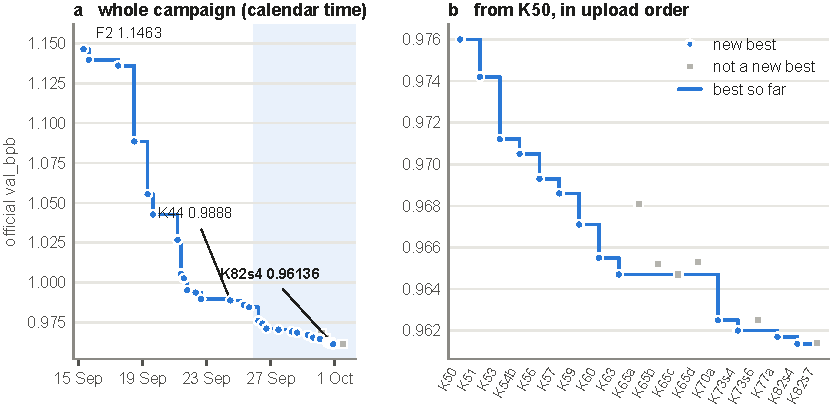
\includegraphics[width=\linewidth]{score_history.pdf}
  \caption{\textbf{Official score per upload.} (a) The whole campaign in calendar time; the line is the best score
    so far and the shaded region is shown in (b). (b) From \upl{K50} on, in upload order. Circles set a new best;
    squares did not: four official tests of single changes (\upl{K65a}--\upl{K65d}) and two shuffle-salt draws
    (\upl{K73s6}, \upl{K82s7}). The change behind each new best is listed in \cref{tab:uploads}. Source:
    \texttt{results/official-scores.csv}.}
  \label{fig:history}
\end{figure}

\paragraph{Contributions.} The same four contributions, in this order, structure the paper.
\begin{itemize}
  \item \textbf{C1: How well deterministic rehearsal predicts a leaderboard} (\cref{sec:oracle}). A cold,
    full-budget rehearsal of the exact upload file, scored on the first \val{eval-tokens} public validation tokens,
    predicted the official score up to an offset of \val{off-mean-since} (SD \val{off-sd-since}, $n=\val{off-n-since}$).
    The offset is mostly text (the official shard is harder than the first 2M public tokens) but carries a
    per-instance component of a few $10^{-4}$. A calibration frozen on the chip-C calibration uploads predicted the
    seven final uploads with MAE \val{holdout-mae} and a positive bias on faster instances; we report how much of
    this depends on one normalised rehearsal, on salt selection and on the burn-in of the interval.
  \item \textbf{C2: A run simulator, with baselines} (\cref{sec:sim}). \ffsim{} decomposes a score into steps,
    computed by replaying the training script's charged-time schedule, and quality per step, from a ridge surrogate
    fitted on \val{q-nfit} fully specified chip runs out of \val{ds-n} harvested records. Held out pair by pair it
    beats a steps-only baseline and a majority-sign baseline on recipe changes; forward in time its knob features add
    little; on new mechanisms it is no better than chance. A GPU proxy that replays the chip's schedule is a
    feasibility demonstration.
  \item \textbf{C3: An accounting of what moved the score} (\cref{sec:price,sec:findings}). One price,
    $\kappa=\val{kappa}$ bpb per unit $\ln(\text{steps})$, converts every change into optimizer steps. With it we
    report the levers with their noise, a row-level shuffle pool (\val{rowpool-chip} on chip,
    \val{rowpool-official} officially, one pair each), a compilation-accounting trap that only cold rehearsals
    reveal, the size of seed and order noise, negative results, and a pricing of the gap to the top ten
    (\val{gap-ten-range} more effective compute) that we offer as a hypothesis about kernels, not a finding.
  \item \textbf{C4: Released artifacts} (\cref{sec:contrib}). The simulator, the run dataset, both recipes, a
    local app and a reviewed, guarded pipeline through which others can add runs to the simulator. No external
    contributions exist yet.
\end{itemize}

\paragraph{Scope.} This is one team's campaign on one contest and one hardware type, and most late effects rest on
one or a few same-seed pairs at a seed that was itself selected. We give $n$ and a noise scale for every effect, mark
numbers that exist only in campaign documents with a dagger (\docnum{}, listed in \cref{app:docfacts}), and list the
threats to validity in \cref{sec:limits}. Other teams appear only as rank-indexed scores from the public leaderboard
snapshot.

\paragraph{Roadmap.} \Cref{sec:related} places the work in context. \Cref{sec:setting} describes the contest, the
determinism the method relies on, the price of a step and our final recipe (\cref{sec:recipe}). \Cref{sec:oracle,sec:sim} present C1
and C2, \cref{sec:findings} C3, \cref{sec:contrib} C4 and \cref{sec:limits} the limitations. The appendices hold the
upload ledger (\cref{app:ledger}), oracle details (\cref{app:oracle}), the simulator internals, the
contribution pipeline, the final hyperparameters, derivations and a notation table.

% sections/related.tex
\section{Related work}
\label{sec:related}

\paragraph{Speed-runs and time-to-result benchmarks.} The GPT-2-small speed-run lineage starts from nanoGPT
\citep{karpathy2022nanogpt} and the GPT-2 recipe \citep{radford2019gpt2}; the modded-nanoGPT records
\citep{jordan2024moddednanogpt} turned it into a public race on FineWeb-style data \citep{penedo2024fineweb}.
Academic work on fixed-budget training includes cramming a BERT in one GPU-day \citep{geiping2023cramming}, BERT on
an academic budget \citep{izsak2021academic} and budget-aware schedules \citep{li2020budgeted}. MLPerf Training
\citep{mattson2020mlperf} and AlgoPerf \citep{dahl2023algoperf} formalise time-to-result benchmarking and discuss
the run-to-run variance and the workload-specific tuning it invites; AlgoPerf is the closest analogue to a
wall-clock contest. Our setting adds a graph compiler inside the charged clock and an organiser-scored shard, and
we contribute measurements of the evaluation loop rather than a recipe.

\paragraph{Leaderboards, adaptive reuse and selection.} Reusing a hold-out set for many adaptive decisions
overfits it; the reusable hold-out \citep{dwork2015reusable} and the Ladder mechanism \citep{blum2015ladder} limit
what a leaderboard reveals for this reason. A meta-analysis of Kaggle competitions \citep{roelofs2019metaanalysis}
found such overfitting smaller in practice than worst-case theory suggests, and model-selection bias inflates the
score of whatever is chosen as best \citep{cawley2010overfitting}. These are the right frame for three things we
did: four uploads were official tests of single changes (\cref{sec:limits}), seeds and shuffle salts were chosen
by their rehearsal score (a winner's curse, \cref{sec:salts}), and the rehearsal scores the public text that may
overlap the official shard (\cref{sec:contest}).

\paragraph{Optimizers, schedules and instability.} Our recipe uses Muon, momentum orthogonalised by a Newton--Schulz
iteration \citep{jordan2024muon,bjorck1971orthogonal}, for matrices and AdamW
\citep{kingma2015adam,loshchilov2019adamw} for the rest. Muon is analysed as steepest descent under a spectral norm
by \citet{bernstein2024anthology,bernstein2024modular}; scaling studies and variants include
\citet{liu2025muonscalable} and NorMuon \citep{li2025normuon}. Warm-up and decay follow the warmup-stable-decay and
cooldown literature \citep{loshchilov2017sgdr,hu2024minicpm,hagele2024scaling,defazio2024schedulefree}. Why warm-up
stabilises early training is analysed by \citet{liu2020radam} and \citet{xiong2020layernorm}; loss spikes and
instabilities in early or large-scale training are studied by \citet{wortsman2024proxies}, \citet{chowdhery2023palm},
\citet{molybog2023adam} and \citet{takase2025spike}. Our warm-up ``spike path'' (\cref{sec:seeds}) is a small-scale
instance. The batch warm-up follows the critical-batch-size view \citep{mccandlish2018largebatch} and
linear-scaling practice \citep{goyal2017imagenet}.

\paragraph{Scaling laws and the price of compute.} Power laws in compute \citep{kaplan2020scaling} and
compute-optimal allocation \citep{hoffmann2022chinchilla} describe loss as a function of model size and tokens;
\citet{hagele2024scaling} extend them to runs whose length is set by a cooldown. Our price of a step
(\cref{sec:price}) is the same object seen locally, the slope of score in log steps at one operating point, used to
price engineering changes.

\paragraph{Weight averaging, data order and architecture.} Our final weights blend live weights with an
exponential moving average \citep{polyak1992averaging,izmailov2018swa,kaddour2022lawa,sanyal2023earlyavg,moralesbrotons2024ema,busbridge2023ema}.
Random reshuffling beats with-replacement sampling \citep{gurbuzbalaban2019reshuffling,mishchenko2020reshuffling},
partial shuffles trade I/O for statistical quality \citep{xu2022corgipile}, and packing and document boundaries
affect language-model quality \citep{krell2021packing,zhao2024sequence,ding2024truncations}; our row pool is a
row-level shuffle buffer on a streaming loader. The architecture uses attention \citep{vaswani2017attention} with
rotary embeddings \citep{su2021roformer}, grouped-query attention with one key/value head
\citep{shazeer2019mqa,ainslie2023gqa}, a squared-ReLU-family MLP \citep{so2021primer}, value embeddings related to
value-residual learning \citep{zhou2024valueresidual} and multi-token prediction \citep{gloeckle2024multitoken};
attention-source reuse is closest to cross-layer attention sharing \citep{brandon2024cla,xiao2019sharing}.

\paragraph{Performance models and learning-curve surrogates.} Step time has been predicted analytically and from
learned models: the roofline model \citep{williams2009roofline}, Paleo \citep{qi2017paleo}, cost predictors
\citep{justus2018predicting}, a learned TPU cost model \citep{kaufman2021tpu} and Habitat \citep{yu2021habitat}.
Throughput and utilisation work \citep{narayanan2021megatron,korthikanti2023recompute,dao2022flashattention,dao2023flashattention2,chowdhery2023palm}
motivates separating step time from per-step quality. Learning-curve extrapolation
\citep{domhan2015extrapolating,swersky2014freezethaw,klein2017lcbnn,adriaensen2023lcpfn} and multi-fidelity search
\citep{li2018hyperband,falkner2018bohb} predict final loss from partial runs. \ffsim{} is simpler: a linear model on
recipe features with an explicit step term, fitted on full runs only, because in our data short screens predict
early loss but not the final ranking.

\paragraph{Variance, determinism and reproducibility.} Seed and data-order variance can rival the effects being
studied \citep{picard2021seed,dodge2020finetuning,bouthillier2021variance}, and implementation-level nondeterminism
adds more \citep{pham2020variance,nagarajan2018deterministic,zhuang2021randomness,summers2021nondeterminism}; PyTorch
documents which operations can be made deterministic \citep{pytorch_reproducibility}. Our protocol depends on the
accelerator being deterministic for a fixed file and seed (\cref{sec:determinism}).

\paragraph{Trainium.} Trainium2 and its NeuronCore-v3 are documented by AWS
\citep{aws_trainium,aws_trainium2_arch,aws_trn2_arch,aws_neuroncore_v3}; programs are compiled by the Neuron
compiler \citep{aws_neuron_docs} and custom kernels are written in NKI \citep{aws_nki_docs}. A search on
1~October 2026 found no peer-reviewed study of small-model training efficiency on this hardware. Other participants
have published write-ups of their own approaches to this contest, for example on co-designing the model and its
kernels \citep{kancharla2026trainiumofthought}.

% sections/setting.tex
\section{Setting}
\label{sec:setting}

\subsection{The contest}
\label{sec:contest}

Phase~1 (Round~1) of the AWS Trainium Frontier challenge \citep{trainiumfrontier2026rules} asked teams to train a
language model from scratch with the organiser's kit\footnote{Provided by the organisers to participants. We
do not redistribute the kit, its data loader or its tokenizer, and our recipes import them.} on a
\texttt{trn2.3xlarge} instance \citep{aws_trn2_arch,aws_trainium2_arch}. The rules that shape everything below are
these.
\begin{itemize}
  \item \textbf{A charged-time budget.} Training may use \val{budget-s}~s (30~minutes) of wall-clock time,
    excluding start-up and compilation \citep{trainiumfrontier2026rules}. The kit runs eight data-parallel ranks
    under \texttt{torchrun}.
  \item \textbf{One file.} A submission is a single \texttt{train.py}, run inside the organiser's harness. The
    submission portal rejected files of \val{size-limit} bytes or more; this limit is not stated in the published
    rules. Our final file is \val{k82-bytes} bytes.
  \item \textbf{The metric.} The score is validation bits per byte ``on the pinned validation shard, computed over
    \textasciitilde20M tokens'' \citep{trainiumfrontier2026rules},
    \begin{equation}
      \label{eq:bpb}
      \text{\valbpb{}} \;=\; \frac{1}{\ln 2}\,\frac{\sum_{t} -\ln p_\theta(x_t \mid x_{<t})}{\text{number of UTF-8 bytes}},
    \end{equation}
    which is independent of the tokenizer; lower is better. \Cref{eq:bpb} is also what our rehearsals compute. The kit also ships public validation
    data, which teams may score locally. Uploads are scored only by the organisers.
  \item \textbf{Deadline and standings.} Round~1 closed at \val{rules-deadline}. The rules limit each team to one
    entry \citep{trainiumfrontier2026rules}; \cref{tab:uploads} lists the official score of each of our uploads. Our
    last upload, \upl{K82s7}, was made at \val{k82s7-upload}, inside the deadline. We report our best scored upload,
    \upl{K82s4} (\val{best-official-long}); our last upload, a shuffle-salt draw of the same recipe, differs from it
    by \val{salt7-vs-salt4}. The top ten teams advanced to Round~2.
\end{itemize}

\paragraph{The evaluation text.} The rules do not say whether the pinned shard is disjoint from the public
validation data. The size of our offset (\cref{sec:oracle}) is consistent with the official score being computed on
text like the first \val{rules-shard-tokens} public validation tokens: the same model scores \val{text-gap}\docnum{}
worse on 20M public tokens than on the first 2M. If the shards overlap, our rehearsals scored part of the official
text, and choosing seeds and shuffle salts by their rehearsal score (\cref{sec:salts}) was selection on part of the
evaluation set. We treat that possibility as a threat to validity throughout rather than rule it out.

\paragraph{Terms.} A \emph{micro-batch} is 65{,}536 tokens across the eight ranks, and $k$ is the number of
micro-batches accumulated per optimizer step. A \emph{step} is one optimizer update. A \emph{rehearsal} is a
full-length run of an exact upload file on our own Trainium instance, scored on the first \val{eval-tokens} tokens of
the public validation data. An \emph{upload} is an officially scored submission, named by our recipe identifier
(\upl{K82s4} is recipe K82 with shuffle salt~4). A \emph{chip} is one of our separate \texttt{trn2.3xlarge}
instances. Chips A--D produced the run records the simulator is fitted on; chips E, G and H were added on the final
day and produced only rehearsals, which are not in the released run dataset (\cref{sec:limits}). Chips differ in step
time by up to \val{chip-spread}\docnum{}, and chip~D's older Neuron runtime (2.33.10, against 2.34.10 on chip~C) was
\val{chip-old-runtime}\docnum{} slower, so we compare step counts only within a chip. Symbols are collected in
\cref{tab:notation} (\cref{app:notation}).

\subsection{Determinism}
\label{sec:determinism}

The Neuron compiler turns the training step into static graphs \citep{aws_neuron_docs}. Two different properties
matter, and we have different evidence for each.
\begin{enumerate}
  \item \textbf{Same trajectory, given the same steps.} Given the same file, seed and data order, the optimizer
    trajectory should be identical. Our direct evidence is one pair: a cold rehearsal and a warm rerun of one file on
    19~September scored \val{det-cold}\docnum{} and \val{det-warm}\docnum{}, a difference of \val{det-diff}. That is
    repeatable to $10^{-5}$, not bit-for-bit, and it rests on $n=1$ with older code. The offset statistics do not
    settle the question: a slope of \val{reg-slope} (\cref{sec:oracle}) shows the offset does not depend on the
    recipe, and the within-chip offset SD (\val{off-sd-within}, 95\% CI \val{off-sd-within-lo}--\val{off-sd-within-hi})
    cannot rule out an official run that re-draws the order noise (expected SD about \val{noise-chip-pair},
    \cref{sec:levers}).
  \item \textbf{Same number of steps.} Training stops at a wall-clock target, so the step count depends on the
    host's speed and on run-to-run jitter. Within a seed sweep (one recipe on one chip; the seed changes neither the
    program nor the step time) the step count has an SD of \val{jitter-sd-lo}--\val{jitter-sd-hi} steps and a range
    of \val{jitter-range-lo}--\val{jitter-range-hi} steps (\texttt{runs.jsonl}). Across chips it differs by up to
    \val{chip-spread}\docnum{}.
\end{enumerate}
The oracle of \cref{sec:oracle} needs the first property and is degraded by the second. Determinism is not the
default on GPUs, where atomics in attention backward passes make repeated runs differ
\citep{pytorch_reproducibility,summers2021nondeterminism}; \cref{sec:gpu} measures that for our GPU proxy.

\subsection{The price of a step}
\label{sec:price}

In a fixed time budget, a change that helps per step but costs step time must pay for itself. We price everything
with one constant.

\begin{center}
\fbox{\begin{minipage}{0.94\linewidth}
\textbf{Definition (price of a step).} Near our operating point, at a fixed recipe and batch schedule,
\begin{equation}
  \label{eq:exchange}
  \Delta\text{bpb} \;\approx\; -\kappa\,\ln\frac{S'}{S}, \qquad \kappa=\val{kappa}\ \text{bpb},
\end{equation}
where $S$ is the number of optimizer steps the budget allows. Equivalently, one percent more steps is worth
$\rho=\kappa/100=\val{xr-step-rate}$~bpb. \emph{Effective compute} means optimizer steps at a fixed recipe and
batch schedule; tokens and FLOPs are then proportional to steps. Every ``step equivalent'', compute ratio and gap
in this paper uses $\kappa=\val{kappa}$, with $[\val{kappa}, \val{xr-k-anchor}]$ as the sensitivity range.
\end{minipage}}
\end{center}

\paragraph{Where $\kappa$ comes from.} $\kappa=\val{kappa}$ is the per-step rate we measured by normalising
same-recipe runs between two chips of different speed\docnum{} (the number of comparisons behind it is not recorded
in the repository, so we give it no confidence interval). A second, independent calibration comes from one
\val{anchor-date} run trained for \val{xr-anchor-long}~s instead of \val{xr-anchor-short}~s
(\val{xr-anchor-pct} more steps at a constant 262k-token batch, before the batch warm-up existed), which improved
\valbpb{} by \val{xr-anchor-gain}\docnum{}. One point and one free parameter is a calibration, not a fit: it gives
$\kappa=\val{xr-k-anchor}$. The law is not constant across the campaign; \cref{app:kappa} gives its curvature and
why the surrogate's slope is not independent evidence for it.

\paragraph{Uses and limits.} \Cref{eq:exchange} prices changes of a few percent, which is how we use it in
\cref{sec:findings}; the simulator builds it into its decomposition (\cref{sec:decomp}). Extrapolations to large gaps (\cref{sec:gap}) are indicative only. One consequence is worth
stating early: a change that costs 1\% of step time must improve per-step quality by at least \val{xr-step-rate}~bpb to
break even, so a per-step gain measured at equal steps, on a GPU proxy for instance, is not a win until its step
cost on the chip is known. \Cref{fig:exchange} (\cref{sec:gap}) shows the law with both calibrations.

\subsection{The final recipe}
\label{sec:recipe}

\Cref{tab:recipe} summarises \upl{K82s4}, our best scored file. It descends from the organiser's GPT baseline, and
every setting is a default in the file (\cref{app:recipe} lists the knobs). Its lineage over the last two days was
\upl{K60} (attention-source reuse) $\to$ \upl{K63} (EMA off, cooldown 0.7, lower learning rate in the small-batch
phases) $\to$ \upl{K70a} (row pool) $\to$ \upl{K73s4} (fused optimizer, a deeper execution queue, a lower MLP
output-projection learning rate, salt~4) $\to$ \upl{K77a} (EMA blend 0.6) $\to$ \upl{K82s4} (EMA prewarm). \Cref{sec:steps} breaks down where
the campaign's extra optimizer steps came from.

\begin{table}[tbp]
  \centering
  \caption{\textbf{The final recipe, \upl{K82s4}.} About \val{params}\docnum{} parameters; every value is a default
    of \texttt{recipes/K82s4/train.py} (full knob list in \cref{tab:hyper}).}
  \label{tab:recipe}
  \small
  \begin{tabular}{@{}p{2.2cm}p{13.6cm}@{}}
    \toprule
    Component & Setting \\
    \midrule
    Model & 9 blocks, width 1{,}024; four 256-wide query heads sharing one key/value head (GQA); value embeddings
      fed to blocks 0 and 8; LeakyReLU(0.35)$^2$ MLP ($4\times$); rotary embeddings with a key offset (radius 0.3);
      blocks 6--8 reuse block~5's attention source (\knob{FF_ATTN_SRC=5:6,7,8}); logit soft cap 15. \\
    Objective & Next-token loss plus a 3-token multi-token-prediction loss with weights 1/0.5/0.25, faded to plain
      next-token prediction in eight stages by 45\% of the run. \\
    Optimizers & Muon (5 Newton--Schulz iterations, fused update) for matrices; AdamW for embeddings, scalars and
      the head; MLP output projection at learning rate $\times0.8$. \\
    Schedule & Charged-time target 1{,}795~s; batch warm-up 65k $\to$ 131k $\to$ 262k tokens per step
      (\knob{FF_ACCUM_SCHED=1:0.06,2:0.2,4}) with learning rate $\times0.35$ and $\times0.6$ in the small-batch phases;
      20 warm-up steps; linear cooldown over the last 70\% of the run. \\
    Data & Stream-row loader; from micro-batch \val{rowpool-from} on, rows are drawn without replacement from a pool
      of \val{rowpool-size} micro-batches (shuffle salt 4). \\
    Final weights & 0.6 blend of live weights and an EMA updated every 32 steps; the EMA update is compiled
      during the excluded start-up (\knob{FF_EMA_PREWARM}). \\
    Seed & 73. \\
    \bottomrule
  \end{tabular}
\end{table}

% sections/oracle.tex
\section{C1: How well full-length rehearsal predicts the leaderboard}
\label{sec:oracle}

\subsection{Protocol}

The rule we followed for every rehearsed upload from 26~September on (all except the four official tests
\upl{K65a}--\upl{K65d}) is short:
\begin{quote}
  Run the \emph{exact upload file}, at the upload seed, on your own Trainium instance, for the full charged budget,
  starting \emph{cold}. Score the trained weights on the first \val{eval-tokens} tokens of the public validation
  data. The official score will be that number plus an offset.
\end{quote}
Each shuffle salt is a code constant, so every salt is its own file with its own hash, and its rehearsal is a
rehearsal of that file. Among the rehearsed uploads, two depart from the rule. The rehearsal of \upl{K70a} ran on
chip~E, which is slow, and was normalised to chip-C speed before use (\cref{sec:k70a}). \upl{K54b} was rehearsed
before its comments were stripped to bring it under the size limit; the uploaded file, \upl{K54b\_min}, parses to the
\val{k54b-ast}\docnum{} as the rehearsed one, so it runs the same program. For upload $i$ with rehearsal
score $r_i$ on chip $c(i)$ and official score $y_i$ we write
\begin{equation}
  \label{eq:offset}
  y_i = r_i + \mu + \gamma_{c(i)} + \varepsilon_i, \qquad \varepsilon_i \sim \mathcal{N}(0, \sigma_{\text{off}}^2),
\end{equation}
where $\mu$ is the part of the offset that belongs to the evaluation text and $\gamma_c$ a per-chip part. During
the campaign we used the special case $\gamma\equiv0$: estimate $\hat\mu$ and $s$ from $n$ earlier uploads and
predict $y_{\text{new}}$ with the interval $r_{\text{new}} + \hat\mu \pm t_{n-1,0.975}\, s\sqrt{1 + 1/n}$
(\cref{app:derivations}). Apart from \upl{K65a}--\upl{K65d}, a file was uploaded only after its cold rehearsal
had exited cleanly, with no graph breaks, charged time inside the budget and the file under the size limit. The
repository records written projections for three uploads (\cref{sec:projections}).

\paragraph{Why it should work, and why not exactly.} If training is deterministic (\cref{sec:determinism}), the
official run follows the rehearsal's trajectory for as many steps as it gets. The text then contributes a
near-constant: the first 2M public tokens are easier than the first 20M by \val{gap-mean} (SD \val{gap-sd} over
\val{gap-n} runs; \cref{sec:contest}), which is the size of the offset. But the official host need not run at the rehearsal chip's
speed. A host that is $x\%$ faster or slower gives $x\%$ more or fewer steps, worth $\rho x$ at the price of
\cref{sec:price}. That is the term $\gamma_c$: it is a property of the \emph{rehearsal chip}, relative to the
official host, not of the text.

\subsection{What the offset is made of}

\Cref{tab:offset-periods} (\cref{app:oracle}) gives the offset by period. Since \upl{K50} the official score has been the rehearsal plus
\val{off-mean-since} (SD \val{off-sd-since}, range \val{off-min-since} to \val{off-max-since},
$n=\val{off-n-since}$). The early uploads, rehearsed on chips A and B with older code and some warm rehearsals, are
noisier (SD \val{off-sd-early}). Two checks support an offset that does not depend on the recipe. The rehearsals
since \upl{K50} span \val{since-rehearsal-span} bpb, and over that range the least-squares slope of official on
rehearsal is \val{reg-slope} (95\% CI \val{reg-lo} to \val{reg-hi}; $r=\val{reg-r}$), consistent with~1
(\cref{fig:oracle}a). The offset shows no significant drift with upload order: \val{trend-slope}$\times10^{-5}$ bpb per
upload (95\% CI \val{trend-lo} to \val{trend-hi}).

The offset was not the same on every chip (\cref{tab:offset-chips}). Chip~C, on which the calibration uploads
were rehearsed, averaged \val{chip-off-c} ($n=\val{chip-off-n-c}$); chip~H \val{chip-off-h} ($n=2$); chip~G, the
fastest final-day instance, \val{chip-off-g} ($n=3$). Within chips the SD is \val{off-sd-within}, smaller than the
pooled \val{off-sd-since}. Rounding and the run-to-run variation of the text gap explain little of the within-chip SD (\cref{app:offset-detail}). Predicting each upload
leave-one-out from the other uploads on its own chip, where there is one, gives an MAE of \val{loo-chip-mae} against
\val{loo-pooled-mae} for the pooled mean ($n=\val{loo-n}$). The offset may therefore be better described as text plus
chip, as in \cref{eq:offset}, than as a property of the text alone. With two or three uploads per new chip,
$\gamma_c$ cannot be estimated well; a step-normalised rehearsal would remove it at the source.

\paragraph{Chip or model quality?} On the final day the faster chips also rehearsed the better recipes and the
lottery winners. The uploads rehearsed on chips G and H have a mean offset \val{cq-gh-diff} above the rest, but given
the rehearsal score the G/H term is \val{cq-gh-coef} ($p=\val{cq-perm-p-adj}$; \cref{app:offset-detail}), so the
offset only \emph{may} depend on the chip.

\begin{table}[tbp]
  \centering
  \caption{\textbf{Offset by rehearsal chip since \upl{K50}} ($10^{-3}$ bpb). ``Frozen-fit error'': mean error of the
    frozen chip-C calibration (\cref{tab:offset-holdout}) on that chip's final-day uploads.
    \textsuperscript{s}\,salt chosen by a lottery; \textsuperscript{i}\,salt inherited from a lottery winner;
    \textsuperscript{n}\,rehearsal normalised to chip-C speed.}
  \label{tab:offset-chips}
  % GENERATED by paper/analysis -- offset by rehearsal chip since K50, 1e-3 bpb (oracle.py)
{\small
\begin{tabular}{@{}lp{5.4cm}rrrr@{}}
\toprule
Chip & Uploads since K50 & $n$ & Mean & SD & Frozen-fit error \\
\midrule
B & K50 & 1 & \ensuremath{+}6.86 & -- & -- \\
C & K51, K53, K54b, K56, K57, K59, K60, K63 & 8 & \ensuremath{+}6.52 & 0.39 & \ensuremath{-}0.04 \\
E & K70a\textsuperscript{n} & 1 & \ensuremath{+}6.55 & -- & \ensuremath{+}0.03 \\
H & K73s4\textsuperscript{s}, K82s4\textsuperscript{i} & 2 & \ensuremath{+}6.84 & 0.07 & \ensuremath{+}0.31 \\
G & K73s6\textsuperscript{s}, K77a\textsuperscript{i}, K82s7\textsuperscript{s} & 3 & \ensuremath{+}7.12 & 0.21 & \ensuremath{+}0.59 \\
\bottomrule
\end{tabular}
}

\end{table}

\begin{figure}[tbp]
  \centering
  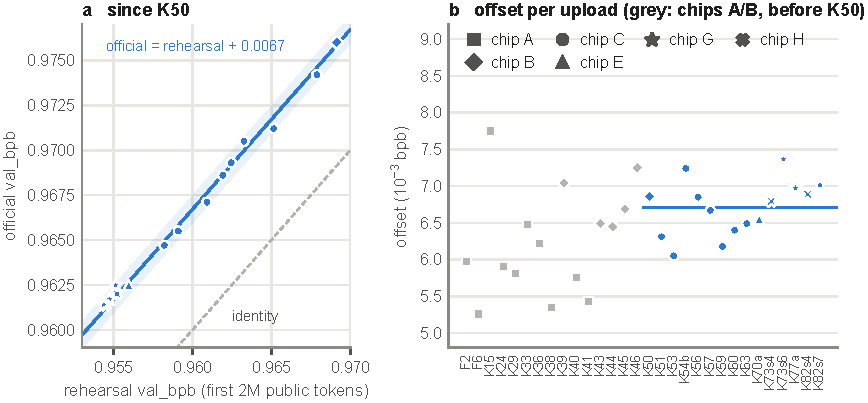
\includegraphics{oracle_calibration.pdf}
  \caption{\textbf{Rehearsal and official score.} (a) Rehearsal against official for the \val{off-n-since} uploads
    since \upl{K50}; the solid line is official $=$ rehearsal \val{off-mean-since-short} with a $\pm2$\,SD band,
    the dashed line is identity. (b) The offset per upload in upload order; grey marks the early chip-A/B uploads.
    Marker shape is the rehearsal chip.}
  \label{fig:oracle}
\end{figure}

\subsection{Pseudo-prospective checks}
\label{sec:oracle-holdout}

Calibration on the uploads it describes is not a test. We therefore predict each upload only from uploads that came
before it. These analyses are computed now from the released ledger, without access to later data, so they are
leakage-free \emph{retrospective} simulations of the protocol, not archived prospective predictions.

\paragraph{Frozen calibration.} The simulator's offset model is fitted on the seven chip-C calibration uploads
\upl{K51}--\upl{K60} ($\hat\mu = \val{frozen-offset}$), the last of them scored on 29~September, before any final-day
upload. \Cref{tab:offset-holdout}
applies it, frozen, to the seven final-day uploads, which were rehearsed on four chips. The MAE is
\val{holdout-mae}~bpb (95\% bootstrap \val{holdout-mae-lo}--\val{holdout-mae-hi}), against \val{nooffset-mae} for no
offset at all, \val{priormean-mae} for the mean offset of all \val{priormean-n} earlier rehearsed uploads
(\val{priormean-offset}), \val{earlymean-mae} for the mean of the \val{earlymean-n} early chip-A/B uploads alone, and
\val{priorsince-mae} for the mean of the \val{priorsince-n} earlier uploads since \upl{K50}: the frozen fit, whose
window and calibration set were chosen with the data in view (\cref{sec:limits}), does no better than that plain
mean. The bias is \val{holdout-bias}: \val{holdout-npos}
of the 7 errors are positive (one-sided sign test $p=\val{holdout-signp}$), and the mean error is
\val{chip-ferr-c} on chip~C, \val{chip-ferr-h} on chip~H and \val{chip-ferr-g} on chip~G. This is the pattern
\cref{eq:offset} predicts for a calibration that sets $\gamma_c$ to chip C's value: the faster final-day chips
look ``hotter''.

\begin{table}[tbp]
  \centering
  \caption{\textbf{Frozen chip-C calibration} ($\hat\mu=\val{frozen-offset}$, fitted on \upl{K51}--\upl{K60}) applied to
    the final-day uploads. Error $=$ official $-$ (rehearsal $+\hat\mu$), in $10^{-3}$ bpb. Marks as in
    \cref{tab:offset-chips}. \upl{K82s4} and \upl{K82s7} were published to seven decimals
    (\val{best-official-long} and \val{salt7-official-long}).}
  \label{tab:offset-holdout}
  % GENERATED by paper/analysis -- frozen chip-C offset applied to the final-day uploads (oracle.py)
{\small
\begin{tabular}{@{}lcrrrr@{}}
\toprule
Upload & Chip & Rehearsal & Predicted & Official & Error ($10^{-3}$) \\
\midrule
K63 & C & 0.958210 & 0.96474 & 0.9647 & \ensuremath{-}0.04 \\
K70a\textsuperscript{n} & E & 0.955946 & 0.96247 & 0.9625 & \ensuremath{+}0.03 \\
K73s4\textsuperscript{s} & H & 0.955209 & 0.96174 & 0.9620 & \ensuremath{+}0.26 \\
K73s6\textsuperscript{s} & G & 0.955138 & 0.96167 & 0.9625 & \ensuremath{+}0.83 \\
K77a\textsuperscript{i} & G & 0.954729 & 0.96126 & 0.9617 & \ensuremath{+}0.44 \\
K82s4\textsuperscript{i} & H & 0.954472 & 0.96100 & 0.9614 & \ensuremath{+}0.36 \\
K82s7\textsuperscript{s} & G & 0.954379 & 0.96091 & 0.9614 & \ensuremath{+}0.49 \\
\midrule
MAE / bias & & & & & 0.35 / \ensuremath{+}0.34 \\
\bottomrule
\end{tabular}
}

\end{table}

\paragraph{Selection.} Salt lotteries select draws whose rehearsal advantage partly does not transfer
(\cref{sec:salts}), so selected uploads should miss upward. Three final-day uploads had their salt chosen by a
lottery (\upl{K73s4}, \upl{K73s6}, \upl{K82s7}; MAE \val{holdout-mae-direct}); two inherit the winning salt~4
(\upl{K77a}, \upl{K82s4}; \val{holdout-mae-inherited}); only \upl{K63} and \upl{K70a} come from no lottery
(\val{holdout-mae-none}), and one of those is normalised. Chip and selection are confounded here: two of the three
chip-G uploads are lottery winners.

\paragraph{The normalised rehearsal of \upl{K70a}.} \upl{K70a} was rehearsed on the slow chip~E and normalised to
chip-C speed with $\rho$, after the fact (\cref{sec:k70a}). With its raw rehearsal the since-\upl{K50} SD rises from
\val{sens-used-sd} to \val{sens-raw-sd} and the frozen MAE from \val{sens-used-mae} to \val{sens-raw-mae}
(\cref{tab:oracle-sens}), so the headline numbers depend on that normalisation, which is itself an application of
$\rho$.

\paragraph{Expanding window.} Predicting each upload from the mean offset of all earlier uploads since \upl{K50},
with a $t$ prediction interval and a burn-in of three, puts all \val{seq-inside} of \val{seq-n} predictions inside
their 95\% interval (\val{seq-expected} expected), with MAE \val{seq-mae} and bias \val{seq-bias}
(\cref{fig:offset-prospective}). With so few points this is weak evidence: at a burn-in of three the interval uses
$t_{2,0.975}=\val{t-two}$ and is very wide; \cref{app:oracle} gives the coverage at other levels and burn-ins.

\paragraph{The written projections.} Three projections were written before upload; \cref{sec:projections}
compares them with the official scores and explains why we treat their closeness as anecdote.

\subsection{Resolution}
\label{sec:resolution}

The oracle predicts one upload with a 95\% half-width of about \val{pi-half}~bpb ($n=\val{off-n-since}$). A
\emph{difference} between two uploads, if their errors are independent, has SD $\sqrt2\,s=\val{diff-sd}$, so the
oracle resolves official differences of about \val{diff-95}~bpb at 95\%, or about \val{diff-95-within} when both
uploads were rehearsed on the same chip. Rank order is an easier test: of the \val{conc-n} pairs of uploads since
\upl{K50}, the rehearsals ordered \val{conc-agree} the same way as the official scores (\val{conc-ties} official tie,
\val{conc-disagree} reversals), but of the \val{conc-close-n} pairs whose rehearsals differed by less than
\val{conc-close-thr}~bpb only \val{conc-close-agree} were ordered correctly. Most late levers are \val{late-lever-range}~bpb (\cref{tab:levers}). The oracle could
not have \emph{measured} them; what it did was translate chip comparisons, which do not carry the offset's noise,
onto the official scale. The levers themselves were judged on same-seed chip pairs, whose noise is discussed in
\cref{sec:seeds}.

\subsection{Traps}
\label{sec:traps}

The protocol is exact only if the rehearsal is a faithful replica of the official run. Four departures cost us
before we understood them (\cref{app:traps}): one-time compilation after the clock starts, which a warm rehearsal
does not pay (the EMA trap of \cref{sec:prewarm}); a rehearsal chip faster or slower than the official host
($\gamma_c\neq0$); a change to steps 0--19 that moves a seed onto another warm-up path, so that a measured difference
becomes a seed effect; and a time target that is a budget, not a promise. Two organiser-side anomalies are excluded
from all calibration statistics (\cref{app:traps}).

\paragraph{How we used it.} Beyond gating uploads, the oracle let us compare structural changes on chip, against a
same-chip control, without spending an upload, and run lotteries over shuffle salts and seeds; a selected draw gives
back part of its edge (\cref{sec:salts}).

% sections/simulator.tex
\section{C2: \texorpdfstring{\ffsim}{ffsim}, a run simulator}
\label{sec:sim}

The oracle answers ``what will this file score?'' for the price of a full chip run. \ffsim{} tries to answer it for
the price of a millisecond, and to say when it cannot.

\subsection{Decomposition}
\label{sec:decomp}

Because the contest charges wall-clock time, a recipe's score has two sources: how many optimizer steps fit in the
budget, and how much each step learns. \ffsim{} models them separately:
\begin{align}
  y &= q(\text{recipe}, S, \text{seed}) + \mu, \label{eq:decomp}\\
  S &= \operatorname{walk}\bigl(\text{schedule},\; T - t_{\text{res}},\; \{\bar t_k\}_{k\in\{1,2,4\}}\bigr), \notag
\end{align}
where $y$ is the official score, $q$ the rehearsal \valbpb{} after $S$ steps, $\mu$ the offset of \cref{eq:offset}
(with $\gamma_c=0$ for chip~C), $T$ the charged-time target, $t_{\text{res}}=\val{reserve-s}$\docnum{}~s the
measured stop reserve, and $\bar t_k$ the step time of the phase that accumulates $k$ micro-batches. The walk
replays the training script's clock logic: warm-up at the full batch until step~20, each accumulation phase until
its fraction of $T$, the cooldown and the stop rule. \Cref{eq:decomp} makes the trade of \cref{sec:price} explicit:
a change enters through $\bar t_k$ (and so $S$) and through $q$. The step times $\bar t_k$ come from an empirical
step-time model on code-lineage and knob features; with one code lineage left out, it predicts the $k\!=\!4$ step time
of runs whose mechanisms another lineage carried, with an MAE of \val{st-lolo-reach} (\cref{app:steptime} describes
the model and the walk).

\subsection{Data}
\label{sec:simdata}

\texttt{research/sim-data/runs.jsonl} holds \val{ds-n} run records from \val{ds-chips} Trainium instances (chips
A--D; \val{ds-nochip} records have no recorded chip): \val{ds-full} full runs and \val{ds-screens} short screens
(\cref{tab:dataset}), merged from a run table, the campaign ledger and harvested chip logs (\cref{app:simdata}).
\texttt{validation-pairs.json} holds \val{ds-pairs} treatment/control pairs from \val{ds-pair-families} families:
\val{ds-pairs-recipe} recipe changes, each at one seed on one chip, and \val{ds-pairs-noise} comparisons of identical
recipes, \val{ds-pairs-diffseed} across seeds on one chip and \val{ds-pairs-crosschip} across chips at one seed. They
were listed by hand from the campaign log of \val{pairs-listed}\docnum{} (\cref{app:simdata}). The quality model is
fitted only on the \val{q-nfit} full chip runs whose complete environment is known. The final-day runs on chips E, G
and H are not in the dataset.

\subsection{The quality surrogate}
\label{sec:quality}

The quality model is a Bayesian ridge (MAP) regression of the rehearsal score,
\begin{equation}
  \label{eq:quality}
  q = \alpha_{\text{era}} + \delta_{\text{chip}} + b L + c L^2 + \sum_j \beta_j x_j(\text{knobs}) + u_{\text{seed}} + \varepsilon_q,
  \qquad L = \ln(S/2300),
\end{equation}
where 2{,}300 steps is the typical step count of the late recipes, so the intercepts are scores at that step count.
Every coefficient has a Gaussian prior. The components are:
\begin{itemize}
  \item \textbf{Era effects} $\alpha$, one per code era (a group of code versions, \cref{app:sim}). A leakage guard
    merges an era with fewer than two runs into its parent lineage, so that a single-run treatment cannot be absorbed
    by ``its'' era.
  \item \textbf{Chip effects} $\delta$ (prior SD \val{q-prior-chip}) for every instance other than chip~C.
  \item \textbf{A step term} with a strong prior, $b\sim\mathcal{N}(\val{q-prior-b}, \val{q-prior-b-sd}^2)$ and
    $c\sim\mathcal{N}(\val{q-prior-c}, \val{q-prior-c-sd}^2)$, centred on the price of \cref{sec:price}. The prior is
    strong because within an era the step count varies mostly through mechanisms that also change quality. The
    posterior slope, \val{q-slope} per unit $L$, stays close to it and is not independent evidence for $\kappa$.
  \item \textbf{Knob features} $x_j$: \val{q-nbase-features} documented encodings of the knobs that varied, each
    centred on a reference recipe and scaled so that one unit is a typical campaign move (prior SD
    \val{q-prior-knob} bpb per unit; \cref{tab:features}), plus \val{q-nbowl-features} ``bowl'' terms that give tuned
    scalars a non-negative curvature.
  \item \textbf{Seed effects} $u$ (prior SD \val{q-prior-seed}).
\end{itemize}
The fit is a MAP solve with non-negative bowl terms and an empirical-Bayes residual SD, floored at
\val{q-sigma-floor} (\cref{app:fit}). The final $\hat\sigma_q=\val{q-sigma}$ sits on the floor; without the floor the
estimate is \val{q-sigma-nofloor}. For every candidate the model also reports
\emph{support}: whether each changed value was seen in the data, interpolated, extrapolated or never varied. In the
decision rule we used, only a supported candidate whose paired difference from the base is $-0.0003$ or better earns
a chip run. \texttt{simulate} and \texttt{search} propagate the noise by paired Monte Carlo (\cref{app:fit}).

\subsection{Validation, with baselines}
\label{sec:simval}

\Cref{tab:sim-calibration} collects the checks. Every row predicts the difference $\Delta$ between the two arms of a
pair, and sign agreement counts a predicted sign that matches the measured one. Four baselines use the same pairs and
the same leave-one-pair-out protocol: a leave-one-out majority sign, the zero predictor, the mean $\Delta$ of the
other pairs in the same family that share no run with the held-out pair (the mean of all recipe pairs for the
\val{base-fam-nfallback} pairs without one), and the same model with every knob effect switched off (era, chip, steps
and seed only). Intervals are cluster bootstraps over the \val{lopo-boot-clusters} control runs, many of which anchor
several pairs.

\begin{table}[tbp]
  \centering
  \caption{\textbf{Quality-surrogate calibration and baselines.} Sign agreement on treatment/control pairs; MAE of the
    predicted difference in $10^{-3}$ bpb. $\hat\Delta$: predicted, $\Delta$: measured difference. ``Recipe pairs''
    exclude the \val{ds-pairs-noise} seed and chip pairs, on which sign agreement is meaningless. Sign intervals are
    cluster bootstraps over control runs; for the majority sign, each pair's leave-one-out prediction is held fixed
    and the control-run clusters are resampled. The temporal rows compare the surrogate with the steps-only model and
    the zero predictor fitted and scored on the same pairs. \textsuperscript{$\dagger$}\,Per-pair values from
    \texttt{docs/simulator-report-20260929.md}, scored by \texttt{paper/analysis/simulator.py} (\cref{tab:postfit});
    its interval is a Wilson interval, too narrow because several pairs share a control.}
  \label{tab:sim-calibration}
  % GENERATED by paper/analysis -- quality surrogate calibration with baselines (simulator.py)
{\footnotesize
\begin{tabular}{@{}p{7.6cm}rrcr@{}}
\toprule
Check & Pairs & Sign & 95\% CI & MAE ($10^{-3}$) \\
\midrule
\multicolumn{5}{@{}l}{\emph{Full surrogate}} \\
\quad in-sample (reference only) & 99 & 86.9\% &  & 0.21 \\
\quad leave one pair out (LOPO), all pairs & 99 & 84.8\% & 76\%--91\% & 0.39 \\
\quad LOPO, recipe pairs only & 87 & 82.8\% & 73\%--89\% & 0.37 \\
\quad LOPO, recipe pairs with $|\hat\Delta|\ge0.3$ (decision-relevant) & 55 & 92.7\% & & \\
\quad LOPO, recipe pairs with $|\Delta|\ge0.3$ (outcome-decisive) & 52 & 96.2\% & & \\
\quad leave one knob value out (LOKVO), recipe pairs & 87 & 81.6\% &  & 0.58 \\
\multicolumn{5}{@{}l}{\emph{Baselines, same pairs and protocol}} \\
\quad steps + era + chip + seed, knob effects off (LOPO), recipe & 87 & 66.7\% & 51\%--79\% & 0.71 \\
\quad \quad recipe pairs with $|\hat\Delta|\ge0.3$ & 36 & 75.0\% & & \\
\quad leave-one-out majority sign, recipe pairs & 87 & 62.1\% & 48\%--84\% & -- \\
\quad zero predictor ($\hat\Delta=0$), recipe pairs & 87 & -- & & 0.63 \\
\multicolumn{5}{@{}l}{\emph{Forward in time and new mechanisms}} \\
\quad temporal hold-out, fit before 28 Sep & 72 & 86\% & & 0.89 \\
\quad temporal hold-out, fit before 29 Sep & 46 & 91\% & & 0.48 \\
\quad pairs finished after the release fit$^{\dagger}$ & 15 & 53\% & 30\%--75\% & 1.04 \\
\quad \quad zero predictor on the same pairs & 15 & -- & & 0.75 \\
\bottomrule
\end{tabular}
}

\end{table}

\paragraph{Leave one pair out (LOPO).} For each pair, refit without its two runs and predict their difference. On
the \val{lopo-rec-n} recipe pairs the full surrogate agrees on sign \val{lopo-rec-sign} of the time (95\% CI
\val{base-full-rec-signci}) with MAE \val{lopo-rec-mae}. The steps-only baseline scores \val{base-steps-rec-sign}
(\val{base-steps-rec-signci}) and MAE \val{base-steps-rec-mae}; the paired difference, surrogate minus baseline, is
\val{base-diff-sign-ci} of sign agreement and \val{base-diff-mae-ci}$\times10^{-3}$ of MAE. Against the family
mean the surrogate gains \val{base-diff-fam-sign-ci} of sign agreement but no clear MAE gain (\cref{app:pairval}). A majority
sign scores \val{base-major-rec-sign} and the zero predictor has MAE
\val{base-zero-rec-mae} (\cref{fig:pairs} plots every pair). Within the replicate setting of LOPO, then, the knob
features carry real information about signs. On the pairs where the \emph{prediction} is decisive, which is what
the decision rule uses, the surrogate scores \val{lopo-rec-signpdec} on \val{lopo-rec-npdec} pairs against
\val{base-steps-pdec-sign} for the steps-only model (\cref{app:pairval}). The MAE is above the noise floor of two
single runs, \val{pair-noise-floor} (\cref{app:derivations}).

\paragraph{Leave one knob value out (LOKVO).} LOPO measures replicate prediction, since the same knob values usually
stay in the fit through other seeds. LOKVO also drops every run that carries the pair's untried value, so the model
must predict a value it has never seen, which is the question the search asks. Sign agreement on recipe pairs stays
at \val{lokvo-rec-sign} (\val{lokvo-rec-signci}), but the MAE rises to \val{lokvo-rec-mae} (per family in \cref{tab:lopo-family}).

\paragraph{Forward in time.} Fit only on runs before a cutoff and predict every pair dated on or after it, as the
campaign would have (\cref{tab:temporal}). With a cutoff of 29~September the model scores \val{temp-b-sign} on
\val{temp-b-n} pairs, MAE \val{temp-b-mae}; with 28~September, fitted on \val{temp-a-nfit} runs, \val{temp-a-sign}
and MAE \val{temp-a-mae}. The steps-only model fitted on the same early runs scores \val{temp-b-steps-sign} and
\val{temp-a-steps-sign}, so the surrogate gains \val{temp-b-diff-sign-ci} and \val{temp-a-diff-sign-ci} of sign
agreement, but in MAE only with the later cutoff (\cref{app:pairval}). The temporal set excludes the incomplete-knob
runs that tested the newest mechanisms, which biases it towards supported pairs.

\paragraph{A development-set estimate.} The surrogate's specification was not frozen before these checks:
\val{sc-n}\docnum{} configurations were compared with their LOPO results visible (\cref{tab:surrogate-configs},
\cref{app:pairval}), and two feature encodings were set with campaign outcomes in view (named in
\cref{tab:features}). LOPO and LOKVO are therefore development-set estimates; the \val{postfit-n} post-fit pairs
are the only clean test.

\paragraph{Genuinely new mechanisms.} On the \val{postfit-n} pairs that finished after the release fit, which tested
attention-source variants and new learning-rate settings (\cref{tab:postfit}), sign agreement was \val{postfit-sign}
(\val{postfit-k} of \val{postfit-n}; Wilson 95\% interval \val{postfit-wilson}, too narrow because several pairs
share a control), indistinguishable from chance, and the MAE \val{postfit-mae} was worse than the zero predictor's
\val{postfit-zero-mae}. The surrogate can say which knob moves are inside the noise; it cannot say whether a new
mechanism will work. During the campaign we used it for negative screening: none of the \val{search-n}\docnum{} local
candidates around \upl{K60} cleared the chip-confirmation bar, and we ran none of them. Because they were never run,
this is not evidence that they were bad. Every later quality win came from mechanisms the data had never seen (the
row pool and the EMA blend).

\paragraph{A GPU proxy.} A second route replays the chip's optimizer trajectory on a CUDA GPU to measure per-step
quality off the chip; with $n=\val{gpu-n-inf}$ informative pairs and run-to-run noise above its agreement with the
chip, it is a feasibility demonstration, not a validated instrument (\cref{sec:gpu}).

% sections/findings.tex
\section{C3: What moved the score, priced in steps}
\label{sec:findings}

More optimizer steps in the same 30 minutes (\cref{sec:steps}) and a handful of structural changes drove most of the
descent in \cref{fig:history}. This section prices the changes with $\kappa$ (\cref{sec:price}), gives each one a
noise scale (\cref{sec:levers}), examines the row pool, attention-source reuse and the EMA prewarm
(\cref{sec:rowpool,sec:asr,sec:prewarm}) and the noise and selection effects (\cref{sec:seeds,sec:salts}), and ends
with what did not work (\cref{sec:negative}) and what the remaining gap would cost (\cref{sec:gap}).

\subsection{Levers, their noise and their price}
\label{sec:levers}

\Cref{tab:levers} lists the changes that helped. The noise column is the SD of a single measured difference under the
order-redraw noise model of \cref{sec:seeds}: $\sqrt2$ times the shuffle-salt SD for a chip pair
(\val{noise-chip-pair}), plus the offset noise of two uploads for an official pair (\val{noise-official-pair}),
divided by $\sqrt n$ for $n$ pairs. It is the right scale for changes that act after the warm-up; a change that
re-rolls the warm-up path faces the larger seed noise. Four of the six largest effects (multi-token prediction,
batch warm-up, LeakyReLU$^2$, the key offset) come from the campaign log and have no run identifiers in the
repository; the late levers are single pairs at seed~73. Only the row pool, the
attention-source reuse and the earlier, larger levers clear about three noise SDs.

\begin{table}[tbp]
  \centering
  \caption{\textbf{Levers that worked.} $\Delta$: change in \valbpb{} against the lever's control, in $10^{-3}$
    (negative is better). Noise SD: SD of the measured difference ($10^{-3}$, see text). Evidence: ``chip pair'',
    same-seed same-chip rehearsals, raw; ``step-norm.'', normalised for a step-count difference; ``official pair'',
    two uploads that differ by this change. Steps: the step equivalent $\exp(|\Delta|/\kappa)-1$ at
    $\kappa=\val{kappa}$. \textsuperscript{$\dagger$}\,Listed in \texttt{docs/FINDINGS.md} without run identifiers,
    mostly on earlier recipe bases. \textsuperscript{$\ddagger$}\,The batch warm-up changes the step count itself, so
    a step equivalent would double-count.}
  \label{tab:levers}
  % GENERATED by paper/analysis -- levers that worked, docs/FINDINGS.md sections 1 and 3; step equivalent at kappa 0.057
{\footnotesize\setlength{\tabcolsep}{4pt}
\begin{tabular}{@{}p{4.2cm}rrrlrrp{3.3cm}@{}}
\toprule
Lever & $\Delta$ & Noise SD & $|\Delta|/\text{SD}$ & Evidence & $n$ & Steps & Note \\
\midrule
Multi-token prediction (3 tokens, faded) & \ensuremath{-}4.3 & 0.49 & 8.7 & campaign log$^{\dagger}$ & -- & 7.8\% &  \\
Row pool, 256 micro-batches & \ensuremath{-}2.3 & 0.49 & 4.6 & chip pair & 1 & 4.1\% & chip E; official $-$2.2; $-$0.5\% steps \\
Batch warm-up 65k$\to$131k$\to$262k & \ensuremath{-}1.9 & 0.49 & 3.8 & campaign log$^{\dagger}$ & -- & n/a & changes steps itself$^{\ddagger}$ \\
LeakyReLU(0.35)$^2$ MLP & \ensuremath{-}1.7 & 0.49 & 3.4 & campaign log$^{\dagger}$ & -- & 3.0\% & chip C vs ReLU$^2$ $-$1.05; official $-$1.5 \\
Attention-source reuse (6--8 reuse 5) & \ensuremath{-}1.5 & 0.25 & 6.1 & chip pair & 4 & 2.7\% & 3 seeds, 2 chips; 5th pair (s97) $+$1.15 raw; step cost $<$0.1\% \\
Rotary key offset & \ensuremath{-}1.3 & 0.49 & 2.6 & campaign log$^{\dagger}$ & -- & 2.3\% &  \\
Cooldown 0.7 + small-batch LR & \ensuremath{-}0.6 & 0.29 & 2.1 & chip, step-norm. & 3 & 1.1\% & all 3 negative; seeds differ \\
EMA blend 0.6 (no prewarm) & \ensuremath{-}0.5 & 0.49 & 1.0 & chip pair & 1 & 0.9\% & official $-$0.3 (K77a$-$K73s4) \\
MLP output-projection LR $\times$0.8 & \ensuremath{-}0.4 & 0.49 & 0.8 & chip, step-norm. & 1 & 0.7\% & seed 73 only \\
EMA prewarm (K82s4 vs K77a) & \ensuremath{-}0.3 & 0.73 & 0.4 & official pair & 1 & 0.5\% & recovers 15--30 steps \\
\bottomrule
\end{tabular}
}

\end{table}

Three entries need a word. \emph{LeakyReLU(0.35)$^2$} appears with three sizes because they are three comparisons:
\val{lever-leaky}\docnum{} in the campaign log on an earlier base, \val{leaky-chip-c}\docnum{} in a chip-C pair against
ReLU$^2$ at equal steps (the comparison the GPU proxy reproduces), and \val{leaky-official} officially
(\upl{K59}$-$\upl{K57}). \emph{Cooldown~0.7} is reported here together with the lower small-batch learning rate, as three
step-normalised chip pairs\docnum{}, all three negative; \cref{tab:gpu} uses two raw chip pairs of the cooldown change alone,
of opposite sign. The official \upl{K63}$-$\upl{K60} delta (\val{cooldown-official}) is confounded, because
\upl{K63} also turned the EMA off and added 2~s of budget. \emph{Official deltas} between uploads published to four
decimals carry a rounding error of up to $\pm2\times$\val{official-rounding}.

\subsection{The row pool: decorrelating a streaming loader}
\label{sec:rowpool}

\paragraph{Mechanism.} The kit's loader fills each row of a micro-batch from one of several parallel token streams,
so the rows of consecutive micro-batches are contiguous slices of the same few streams. From
micro-batch~\val{rowpool-from} on, our loader instead draws rows without replacement from a look-ahead pool of
\val{rowpool-size} micro-batches (\knob{FF_ROW_SHUFFLE}), a shuffle buffer at row granularity
\citep[cf.][]{xu2022corgipile,mishchenko2020reshuffling}. The first \val{rowpool-from} micro-batches, which cover the
warm-up, are unchanged, so that the seed's warm-up path (\cref{sec:seeds}) is not re-rolled. The shuffle has its own
RNG with a salt, which re-draws the order after micro-batch~\val{rowpool-from} without touching initialisation.

\paragraph{Evidence.} On chip E, the pool scored \val{rowpool-chip-treat}\docnum{} at \val{rowpool-steps-treat}\docnum{}
steps against \val{rowpool-chip-ctrl}\docnum{} at \val{rowpool-steps-ctrl}\docnum{} for the same file without it:
\val{rowpool-chip}\docnum{} raw, about \val{rowpool-stepnorm}\docnum{} after normalising for the
\val{rowpool-step-cost}\docnum{} of steps the pool cost, and about \val{rowpool-z} noise SDs. Officially, \upl{K70a}
scored \val{official-k70a} against \upl{K63}'s \val{official-k63}, a difference of \val{rowpool-official}. That
agreement is what determinism predicts and is not independent evidence that the effect generalises: both numbers come
from the same trajectory pair at seed~73. And because the pool changes the data order, its measured effect contains
one draw of the order noise (SD about \val{salt-sd}\docnum{}). A pool of \val{pool-large}\docnum{} gave the same
result as \val{rowpool-size}; a pool of \val{pool-small}\docnum{} helped less. Other order manipulations were null
within $\pm\val{rowpool-null}$\docnum{}: larger pools, epoch reshuffles, pool-aware accumulation and document
reordering.

\paragraph{What we do not know.} The evidence is one chip pair at one seed and one salt. It is probably real at about
\val{rowpool-z} order-noise SDs, but it is not replicated, and the pair is not in the released run data. Our working hypothesis is
that the pool reduces within-batch correlation between rows of the same stream, and with it gradient variance, in the
spirit of shuffling results for SGD \citep{gurbuzbalaban2019reshuffling}. We have \emph{not} measured this; the checks
are listed in \cref{sec:limits}.

\subsection{Attention-source reuse}
\label{sec:asr}

Blocks 6, 7 and 8 reuse the attention source computed by block~5 (\knob{FF_ATTN_SRC=5:6,7,8}), in the spirit of
cross-layer attention sharing \citep{brandon2024cla,xiao2019sharing}. It is our best-replicated structural effect:
four same-seed chip pairs (seeds 73, 67 and 58 on chip~C, seed~73 on chip~D) gave \val{asr-pairs}\docnum{} (mean
\val{asr-mean}), at a step cost under \val{asr-step-cost}\docnum{}; a fifth pair, seed~97 on chip~D, was
\val{asr-s97-delta}\docnum{} raw, mostly a \val{asr-s97-step-deficit}\docnum{}-step deficit (\cref{tab:postfit}).
Officially, \upl{K60} improved on \upl{K59} by \val{asr-official}. The surrogate, whose coefficient for this feature
then rested on two runs, predicted the right sign on four of five post-fit attention-source pairs but overestimated
the size by about \val{asr-overestimate}\docnum{} (\cref{tab:postfit}).

\subsection{The EMA blend and the prewarm accounting trap}
\label{sec:prewarm}

\paragraph{The trap.} Our final weights are a 0.6 blend of the live weights with an exponential moving average
\citep{polyak1992averaging,moralesbrotons2024ema}. The EMA update is a separate graph. On a fresh instance, the first
EMA update compiles that graph \emph{inside} the charged clock and costs \val{ema-compile-steps}\docnum{} steps. A warm
rehearsal, run after an earlier EMA run on the same instance, finds the graph in the compiler cache and does not pay.
Warm rehearsals therefore looked \val{ema-warm-bias}\docnum{} bpb better than the cold official run would be.

\paragraph{A regression, not a discovery.} The fix, \knob{FF_EMA_PREWARM}, runs one EMA update during the excluded
start-up. It was not new on the final day: the ledger lists the EMA prewarm already in \upl{\val{first-prewarm}}
(26~September). It disappeared when \upl{\val{prewarm-dropped}} turned the EMA off, and \upl{K77a} re-enabled the EMA
without it. Only cold rehearsals exposed the regression, which is the general lesson below.

\paragraph{Evidence.} Step counts on one instance show the cost (\cref{tab:prewarm}). On chip~G the recipe without EMA
ran \val{steps-k73s6} steps, with EMA but without prewarm \val{steps-k77a}, and with both \val{steps-k82s7}; on chip~H,
without EMA \val{steps-k73s4} and with both \val{steps-k82s4}. These are single runs, and step counts jitter by
\val{jitter-range-lo}--\val{jitter-range-hi} steps within a seed sweep (SD \val{jitter-sd-lo}--\val{jitter-sd-hi};
\cref{sec:determinism}). The chip-G drop of \val{prewarm-g-drop} steps without prewarm is about \val{prewarm-g-drop-sds}
single-run jitter SDs but only just above the largest within-sweep range (\val{jitter-range-hi} steps), while the
difference between prewarm and no EMA (\val{prewarm-g-gain} steps on chip G, \val{prewarm-h-gain} on chip H) is inside
it. The salts differ between some of these files, which changes the data order but not the step time.
Officially, \upl{K82s4} (prewarm) scored \val{prewarm-official} against \upl{K77a} (no prewarm): one pair, below the
oracle's resolution (\cref{sec:resolution}), consistent with the step-based estimate. The EMA blend itself is a separate
effect of about \val{ema-blend-chip}\docnum{} in one chip pair without prewarm; officially \upl{K77a} improved on
\upl{K73s4} by \val{ema-blend-official}.

\begin{table}[tbp]
  \centering
  \caption{\textbf{Step counts around the compile trap} (single cold rehearsals, from
    \texttt{results/official-scores.csv}). Compare within a chip only; within-chip jitter is
    \val{jitter-range-lo}--\val{jitter-range-hi} steps.}
  \label{tab:prewarm}
  \small
  \begin{tabular}{llccr}
    \toprule
    Chip & Upload & EMA blend & EMA prewarm & Steps \\
    \midrule
    \val{chip-k73s6} & \upl{K73s6} & -- & -- & \val{steps-k73s6} \\
    \val{chip-k77a} & \upl{K77a} & \checkmark & -- & \val{steps-k77a} \\
    \val{chip-k82s7} & \upl{K82s7} & \checkmark & \checkmark & \val{steps-k82s7} \\
    \midrule
    \val{chip-k73s4} & \upl{K73s4} & -- & -- & \val{steps-k73s4} \\
    \val{chip-k82s4} & \upl{K82s4} & \checkmark & \checkmark & \val{steps-k82s4} \\
    \bottomrule
  \end{tabular}
\end{table}

\paragraph{The general lesson.} Any lazily compiled path that first runs after the clock starts is a hidden cost: EMA
updates, evaluation-mode switches, a late schedule phase with a new batch shape. On a compiled accelerator the compile
cost can exceed the benefit of the feature that triggers it, and only a \emph{cold} rehearsal reveals it. We recommend
that speed-run harnesses either compile all graphs before the clock starts or report compile time separately.

\subsection{Seeds and the warm-up coin flip}
\label{sec:seeds}

The largest single source of variance in our data was not a setting. In warm-up steps 3--10, some seeds take a
\emph{spike path}: the loss falls faster to step~4 and then much more slowly, ending step~10 roughly
\val{spike-gap-nats} nats higher than the good path (\cref{fig:warmup}a). The logged training loss is the weighted
multi-token-prediction sum (weights 1/0.5/0.25), not per-token cross-entropy, which is why it is near 13~nats. We
classify a run as spike-path when its step-10 loss is at least \val{spike-l10} nats. Good-path runs of these recipes
reach \val{l10-good} nats at step~10 and spike-path runs \val{l10-spike}; we chose the threshold after seeing the data,
in the empty gap between them, and one run at \val{l10-mid} is reported as intermediate. On the three clean seed sweeps
of a fixed recipe in our data (\cref{tab:seeds}), \val{spike-k} of \val{spike-n} seeds with a logged curve took the
spike path, \val{spike-frac} (Wilson 95\% interval \val{spike-wilson-lo}--\val{spike-wilson-hi}). The sweeps share
\val{spike-shared-seeds} seed, and the path may be a property of the seed, recipe and hardware together, so the runs
are not fully independent; counting each of the \val{spike-distinct-seeds} distinct seeds once gives
\val{spike-seed-k} spike seeds (\val{spike-seed-wilson}). Spike-path runs ended \val{spike-delta} worse on average
(95\% CI \val{spike-delta-lo} to \val{spike-delta-hi}), smaller than the \val{spike-penalty-doc}\docnum{} we had quoted
during the campaign from a broader, less controlled set of about \val{harvested-runs-doc}\docnum{} runs. We consider the
controlled estimate the better one.

\begin{figure}[tbp]
  \centering
  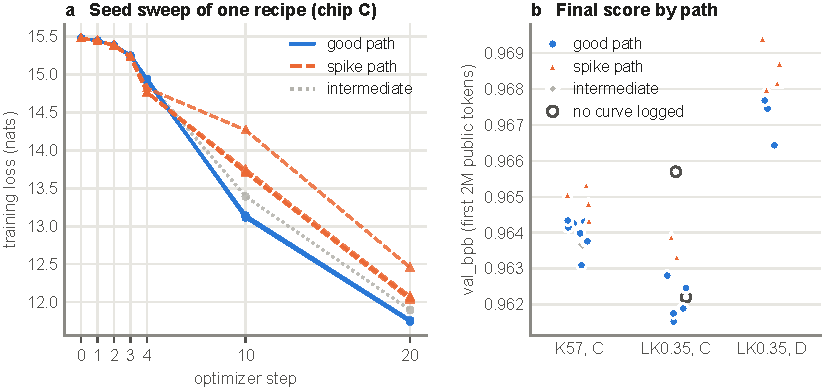
\includegraphics{warmup_paths.pdf}
  \caption{\textbf{The warm-up coin flip.} (a) Training loss (the weighted multi-token sum) over the first 20 steps
    for the \val{g7-nseeds} seeds of one recipe on one chip: spike-path seeds (dashed, triangles) drop faster to
    step~4, then stall. (b) Final score by path in the three seed sweeps; hollow points have no logged curve.}
  \label{fig:warmup}
\end{figure}

\paragraph{The variance budget.} Seeds re-draw the initialisation, the warm-up path and the data order. Within a
sweep, the seed SD is \val{seed-sd-all-lo}--\val{seed-sd-all-hi} including spike paths and
\val{seed-sd-good-lo}--\val{seed-sd-good-hi} among good-path seeds only. Shuffle salts re-draw only the order after
micro-batch~\val{rowpool-from}, with an SD of about \val{salt-sd}\docnum{}. Both are as large as most late
improvements (\cref{tab:levers}).

\paragraph{Selection.} Our seed, 73, was itself chosen by a lottery. In the 13-seed sweep of the \upl{K57} recipe it
ranks \val{g7-s73-rank} of \val{g7-nseeds}, \val{g7-s73-gap} better than the good-path mean, and every later
same-seed comparison is measured on that lottery winner. Effects measured on a selected seed need not hold at other
seeds \citep{cawley2010overfitting}. We followed two rules: a lever must act after step~19, so that it cannot re-roll
the warm-up path, and an effect under 0.0003 needs three seeds; the second was often not affordable. Our one official
test of a change to the first steps illustrates the first rule: an attention-input shift in blocks 6--8 (\upl{K65a})
scored \val{xshift-official} against its base. It may have re-rolled the warm-up path, but we did not log its
step-10 loss, and \val{xshift-official} is about \val{xshift-spike-ratio} times the controlled spike-path penalty
(\val{spike-delta}), so a genuinely harmful change cannot be ruled out.

\subsection{Salt lotteries and the winner's curse}
\label{sec:salts}

Because rehearsals are deterministic, a lottery over shuffle salts can be run on chip and the best rehearsal uploaded.
Four salts of the \upl{K73} recipe spanned \val{salt-span}\docnum{} on chip, and salt~4 was uploaded as \upl{K73s4};
the later uploads \upl{K77a} and \upl{K82s4} inherit it. A second lottery on the final recipe picked salt~7
(\upl{K82s7}); its size is not recorded in the released files. Where a lottery's draws ran on different chips, salt
and chip speed are confounded. Selection was only partly rewarded. Salt~4 kept its edge officially. Salt~6
rehearsed \val{salt6-reh-vs-salt4} against it, but on chip~G against chip~H, so that edge is confounded with the chip;
officially it scored \val{salt6-vs-salt4} against salt~4 (\upl{K73s6}). Salt~7 gave the best rehearsal of the campaign
(\val{salt7-rehearsal}) and tied salt~4 officially (\val{salt7-vs-salt4}).

A simple model explains the pattern. A salt's rehearsal advantage is its true effect (SD about \val{salt-sd-mid}) plus a
part that does not transfer to the official run, with SD $s_\eta$. The expected share of a selected advantage that
survives is the reliability ratio $\lambda$ (\cref{app:derivations}). With $s_\eta$ equal to the final-day offset SD,
$\lambda\approx\val{salt-shrink}$; that SD includes chip-to-chip variation, so we also use the within-chip offset SD
($\lambda=\val{salt-shrink-within}$), the since-\upl{K50} SD and a smaller 0.0002; together they give
$\lambda$ between \val{salt-shrink-lo} and \val{salt-shrink-hi}.
Lotteries are worth running when draws are cheap, but the projected gain should be shrunk by roughly a quarter to a half,
and if the official shard overlaps the public text (\cref{sec:contest}) part of what survives is selection on the
evaluation set itself \citep{dwork2015reusable,blum2015ladder}.

\subsection{What did not work}
\label{sec:negative}

\Cref{tab:negative} lists the changes that lost. Two patterns stand out. First, \emph{capacity changes lost in both
directions}: depth~10 and two key/value heads lost while running \val{depth10-steps}\docnum{} fewer steps, and depth~8
lost despite \val{depth8-steps}\docnum{} more steps. We read this as the 9-block model being a local optimum of the
capacity-for-steps trade at our kernels' speed, but it rests on one or two chip pairs without an equal-step comparison,
so we cannot say whether depth~10 lost \emph{only} because of its steps. Second, \emph{scalar retuning did not pay}:
none of \val{scalar-keys}\docnum{} scalar knob keys (learning-rate scales, betas, weight decay, initialisation,
momentum, soft cap, RoPE base, cooldown $\pm0.1$) won a confirmation. The four official tests on the final day
(\upl{K65a}--\upl{K65d}) were all worse than or tied with their base.

\begin{table}[tbp]
  \centering
  \caption{\textbf{What lost.} $\Delta$ against the control (positive is worse); evidence as in \cref{tab:levers}.
    Official deltas are against \upl{K63}. \textsuperscript{\S}\,May have re-rolled the warm-up path; its step-10 loss
    was not logged (\cref{sec:seeds}). Source: \texttt{docs/FINDINGS.md} \S5\docnum{} and
    \texttt{results/official-scores.csv}.}
  \label{tab:negative}
  % GENERATED by paper/analysis -- what lost, docs/FINDINGS.md section 5 and results/official-scores.csv (K65a-d)
{\small
\begin{tabular}{@{}p{7.6cm}rlr@{}}
\toprule
Change & $\Delta$ ($10^{-3}$) & Evidence & $n$ \\
\midrule
Depth 10 (bigger; 6--11\% fewer steps) & \ensuremath{+}3.8 to \ensuremath{+}4.3 & chip pair & 2 \\
Two KV heads (bigger) & \ensuremath{+}5.7 & chip pair & 1 \\
Depth 8 (smaller; +10.6\% steps) & \ensuremath{+}3.0 to \ensuremath{+}5.0 & chip pair & 2 \\
Late $k{=}8$ batch in the cooldown (K65b) & \ensuremath{+}0.5 & official pair & 1 \\
Split AdamW cooldown 0.4 (K65d) & \ensuremath{+}0.6 & official pair & 1 \\
EMA-Nesterov lookahead 0.3 (K65c) & \ensuremath{+}0.04 & official pair & 1 \\
AdamW LR $-$16\% & \ensuremath{+}0.8 to \ensuremath{+}0.9 & chip pair & 2 \\
AdamW warm-up reshaping (steps 0--19) & \ensuremath{+}1.0 & chip pair & 1 \\
Drop the block-0 MLP & \ensuremath{+}1.9 & chip pair & 1 \\
No positional encoding in layers 3--4 & \ensuremath{+}3.3 & chip pair & 1 \\
Attention-input shift, blocks 6--8 (K65a)$^{\S}$ & \ensuremath{+}3.4 & official pair & 1 \\
Scalar retunes (LR scales, betas, WD, init, momentum, soft cap, RoPE base, cooldown $\pm$0.1) & 0 of 61 keys won & chip pairs & 61 \\
Bigger pools, epoch reshuffles, pool-aware accumulation, document reordering & 0 $\pm$ 0.3 & chip pairs & -- \\
\bottomrule
\end{tabular}
}

\end{table}

\subsection{Pricing the gap in compute}
\label{sec:gap}

\Cref{tab:gap} converts the distance from our best official score, \val{best-official}, to reference points on the final
public leaderboard snapshot (about \val{leaderboard-time}\docnum{}; ranks only) into effective compute through
\cref{eq:exchange}. Closing the \val{gap-ten} gap to \#10 would have needed about \val{gap-ten-range} more effective
compute across our two calibrations of $\kappa$. The gap to \#1, \val{gap-one-range}, extrapolates far beyond the
\val{xr-anchor-pct} anchor and is an order of magnitude only.

\begin{table}[tbp]
  \centering
  \caption{\textbf{What each leaderboard reference would cost in effective compute}, from our best official score
    (\val{best-official}, \upl{K82s4}), as $\exp(\text{gap}/\kappa)-1$ for the price used ($\kappa=\val{kappa}$) and
    for the long-run calibration. Leaderboard values are from the final public snapshot, referred to by rank.}
  \label{tab:gap}
  % GENERATED by paper/analysis -- compute needed = exp(gap / kappa) - 1 (exchange.py)
{\small
\begin{tabular}{@{}lrrrr@{}}
\toprule
Target & val\_bpb & Gap & Compute, $\kappa=0.057$ & Compute, $\kappa=0.063$ \\
\midrule
\#10 on the final snapshot & 0.9554 & 0.0060 & +11\% & +10\% \\
\#1 on the final snapshot & 0.9328 & 0.0286 & +65\% & +58\% \\
\bottomrule
\end{tabular}
}

\end{table}

\paragraph{A hypothesis, not a finding.} The final recipe trained at about \val{tokens-per-s}\docnum{} tokens/s on a
\val{params}\docnum{}-parameter model, which we estimated at roughly \val{mfu}\docnum{} model-FLOPs utilisation
\citep{chowdhery2023palm} with about \val{idle}\docnum{} of wall time idle on host dispatch; both are approximate
profiles. At an equal recipe, \cref{eq:exchange} values \val{tput-lo-pct}--\val{tput-hi-pct}\% more tokens per second
at \val{tput-range}~bpb, more than our whole gap to \#10, while late recipe changes were worth about
\val{late-change}\docnum{} each. We therefore \emph{hypothesise} that the cheapest way to close the gap was kernel
throughput: custom NKI kernels \citep{aws_nki_docs} for attention, the fused MLP and the optimizer updates. Nothing in
our data rules out the alternative that better-ranked teams had better recipes or data handling, and the conversion
assumes that every team sits on our compute curve. A test would be to write one kernel, measure its step time with a
short chip screen, price it with \cref{eq:exchange} and confirm it with a cold rehearsal; we did not reach that stage
in Phase~1.

% sections/contrib.tex
\section{C4: Released artifacts and a guarded contribution pipeline}
\label{sec:contrib}

Almost every record behind \ffsim{} comes from one team's instances and one recipe family, which is the main reason
the surrogate fails on new mechanisms (\cref{sec:simdata,sec:simval}). Other participants hold the data it lacks. We therefore
release, besides the simulator, the run dataset, both recipes, the upload ledger and a local app, a pipeline through
which anyone can contribute the numbers from runs they have already done. It is an artifact, not a result: at the time
of writing no external contribution exists, so we make no claim that the simulator improves with use.

A contribution is one JSON record per run: hardware, time budget, an optional published base recipe plus the knobs
that changed, seed, steps, the local and/or official score, and an explicit consent flag. Every record is checked for
schema, secrets and personal data, plausible knob ranges, duplicates and outliers before a maintainer sees it; an
outlier is flagged for review, never rejected, because a run the model predicts badly is the run it needs. Each
(hardware, base recipe) combination gets its own fixed effect, so a systematic difference between a contributor's
setup and ours is absorbed there rather than in shared coefficients, and one account adds at most \val{guard-cap}
records to a fit. A maintainer's approval opens a pull request with the record exactly as approved, and merging
triggers a refit that is \emph{guarded}: it refuses to write anything if the in-sample or pair-validation error on our
own data grows by more than \val{guard-max-worse}~bpb, or if the prediction for a published base recipe moves by more
than \val{guard-max-shift}~bpb. \Cref{app:contrib} gives the mechanics and a stress test.

The stress test is weak evidence and we present it as such. Its ``honest'' records are generated from the model's own
predictions plus noise, so accepting them is close to automatic; its attack, a coordinated pair of sock-puppet records
that pull a shared coefficient, was designed by us with the thresholds known, and there is no adaptive attacker. The
guard refused that attack down to two records and accepted the honest ones. An attacker who knows the thresholds can
stay under them, and per-hardware effects can absorb slow drifts. What the guard does is turn the cheapest damaging
attack, pulling a shared coefficient, into a visible failure.

% sections/limitations.tex
\section{Limitations and threats to validity}
\label{sec:limits}

\begin{enumerate}
  \item \textbf{Few seeds, at a selected seed.} Most late effects in \cref{tab:levers,tab:negative} are single
    same-seed pairs at seed~73, which ranked \val{g7-s73-rank} of \val{g7-nseeds} in its sweep. Effects measured on
    a lottery winner may not hold at other seeds. The row pool rests on one chip pair and one official pair from the
    same trajectory; the prewarm on one official pair and single-run step counts; the EMA blend on one chip pair. The
    rule we set (three seeds below 0.0003) was often not affordable.
  \item \textbf{Selection and the evaluation text.} Seeds and salts were chosen by rehearsal score, and five of the
    seven final-day uploads carry a lottery-selected salt. Four uploads (\upl{K65a}--\upl{K65d}) were official tests of
    single changes. If the official shard overlaps the public validation text (\cref{sec:contest}), seed and salt
    selection used part of the evaluation set.
  \item \textbf{The offset depends on the chip.} The frozen calibration's errors are positive on the faster
    final-day chips (\cref{tab:offset-chips}), and the oracle's headline statistics depend on one model-normalised
    rehearsal (\cref{tab:oracle-sens}). The pseudo-prospective analyses are retrospective simulations; only three
    written projections are archived.
  \item \textbf{Determinism rests on one pair.} The evidence that a warm and a cold run of one file follow the same
    trajectory is one pair with older code (\cref{sec:determinism}). Step counts jitter by up to
    \val{jitter-range-hi} steps within a chip.
  \item \textbf{Hardware heterogeneity.} Instances differed by up to \val{chip-spread}\docnum{} in step time. We
    normalised only same-recipe runs, never across a change that alters step time, and every comparison in the text
    names its chip.
  \item \textbf{Released data do not cover the final day.} \texttt{runs.jsonl} holds chips A--D up to 29~September.
    The chip E, G and H runs behind the row-pool pair, the salt lottery, the EMA-blend and output-projection pairs, the
    pool-size ablation and the final-day test bench exist only as quotes from campaign documents, marked \docnum{} and
    listed in \cref{app:docfacts}. They are reported, not recomputable.
  \item \textbf{Simulator circularity.} The surrogate was fitted on our own search trajectory: the knobs are
    non-random and confounded with code eras (\cref{tab:coefficients}), and some inputs come from a reconciled campaign
    ledger that was partly extracted from free text (\texttt{research/sim-data/dataset-qa.md}). Its step prior is centred
    on the price it is sometimes used to support. On genuinely new mechanisms it is at chance
    (\val{postfit-sign}, \val{postfit-wilson}).
  \item \textbf{The price of a step.} $\kappa$ rests on a per-step rate whose number of comparisons is not recorded and
    on one long run; it varies with the step count. The gap figures extrapolate it, and other teams' recipes may sit on
    a different curve.
  \item \textbf{Leaderboard snapshot.} The leaderboard references are from the last public snapshot we recorded (about
    \val{leaderboard-time}\docnum{}). The organisers' published final standings may differ.
  \item \textbf{Forking paths.} The campaign was adaptive and the analyses are post hoc; the spike threshold, for
    example, was chosen after seeing the data. The temporal and pseudo-prospective checks are the parts least exposed
    to this. Follow-up experiments should be pre-registered in the repository before they are run.
  \item \textbf{Utilisation estimates.} ``About \val{mfu}\docnum{} MFU'' and ``\val{idle}\docnum{} idle'' are
    approximate profiles. We use them only to motivate the kernel hypothesis of \cref{sec:gap}.
\end{enumerate}

% sections/conclusion.tex
\section{Conclusion}

In a wall-clock contest on a deterministic accelerator, the most useful tool we had was a rule: rehearse the exact
file, cold, and add an offset (C1). It predicted the final uploads to within a few $10^{-4}$, but the offset is part
text and part instance speed, its resolution for differences between uploads is about \val{diff-95}~bpb, and its
best-looking statistics lean on one normalised rehearsal. A simulator that separates the steps a recipe gets from what
each step is worth (C2) beats trivial baselines when it has seen the knob values before and is at chance when it has
not; it says what is noise, not what will work. One price per optimizer step (C3) made every trade explicit, exposed a
compilation regression that only cold rehearsals reveal, and shows that seed, order and selection effects are as large
as most late improvements. Read as a hypothesis, the same accounting puts the gap to the top ten at
\val{gap-ten-range} more effective compute and points at kernels. The data that would test the simulator beyond our
own search belong to other teams, so we release it with a guarded way to contribute (C4).

\paragraph{Release.} The repository contains the simulator (\ffsim{}, MIT), both recipes (Apache-2.0 derivatives of
the organiser's baseline), the run dataset and upload ledger, a local app with prediction and contribution endpoints,
the analysis scripts that generate every number, table and figure in this paper, and the test suite.

% sections/statements.tex
\section*{Reproducibility statement}
\addcontentsline{toc}{section}{Reproducibility statement}

\ifanonymous
The code, data and analysis scripts are in an anonymised repository supplied with the submission:
\else
The code, data and analysis scripts are in the public repository
\url{https://github.com/marker2601/trainium-simulator}:
\fi
\begin{itemize}
  \item \textbf{Data.} \texttt{results/official-scores.csv} (every scored upload with its rehearsal and offset),
    \texttt{research/sim-data/runs.jsonl} (\val{ds-n} run records, chips A--D; \val{ds-nochip} records have no
    recorded chip), \texttt{validation-pairs.json} (\val{ds-pairs} pairs), \texttt{official-uploads.csv}, the
    dataset QA and validation reports, and three reference chip-log directories used by the parsers and tests. Our
    code, data and documents are released under the MIT licence; recipes derived from the organiser's baseline are
    Apache-2.0; contributed records are CC-BY-4.0.
  \item \textbf{Code.} The simulator (\texttt{ffsim/}, numpy only), the GPU proxy (\texttt{ffsim/gpu/}), the app
    (\texttt{space/}), the contribution pipeline (\texttt{ffsim/contrib.py}, \texttt{.github/workflows/}), and both
    recipes byte-identical to the uploaded files, with their SHA-256 hashes in \texttt{recipes/README.md}.
  \item \textbf{Software.} All chip runs used the organiser-provided AWS Neuron environment on \texttt{trn2.3xlarge}:
    PyTorch~2.11.0, \texttt{torch-neuronx}~2.11.3 and the Neuron compiler \texttt{neuronx-cc}~2.26 (build
    2.26.6360.0), with the model compiled by \texttt{torch.compile} (backend \texttt{neuron},
    \texttt{dynamic=False}, the recipes' default), one process per NeuronCore (launch command in
    \texttt{recipes/README.md}). The Neuron runtime was 2.34.10 on chip~C, \val{runtime-chip-a}\docnum{} on chip~A
    and 2.33.10 on chip~D; chips \val{image-chips}\docnum{} were launched from a machine image taken from chip~A and
    so presumably ran the same runtime, but no record from them survives.
  \item \textbf{Commands.} \texttt{pip install -r paper/requirements.txt} installs the pinned dependencies; \texttt{python -m pytest -q tests} runs the test suite;
    \texttt{python paper/analysis/make\_all.py} regenerates \texttt{paper/numbers.tex}, every table in
    \texttt{paper/tables/} and every figure in \texttt{paper/figures/}; \texttt{python paper/check\_tex.py} runs the
    static checks; \texttt{latexmk -pdf main.tex} in \texttt{paper/} builds this document. The analysis is
    deterministic (fixed random seeds, no clock).
  \item \textbf{What is reported but not recomputable.} Numbers marked \docnum{} are quoted from the campaign
    documents in \texttt{docs/} or the campaign log because their raw records are not released: chip-log measurements, the final-day runs
    on chips E, G and H (row-pool pair, salt lotteries, EMA-blend and output-projection pairs, pool-size ablation),
    and the GPU-proxy measurements. \Cref{app:docfacts} lists them with their sources. Official scores come only from
    the organisers. Re-running a recipe needs a \texttt{trn2.3xlarge} instance and the organiser's kit, which we do
    not redistribute; raw chip harvests are withheld because they contain host details.
\end{itemize}

\section*{Ethics and broader impact}
\addcontentsline{toc}{section}{Ethics and broader impact}

\paragraph{Independence.} This is independent work. It is not affiliated with, sponsored by or endorsed by Amazon
Web Services or the contest organisers, and any views and errors are the author's own.

\paragraph{Fair competition and the evaluation data.} All results come from our own submissions. We trained only on
the training data provided by the kit. We scored rehearsals on the first \val{eval-tokens} tokens of the public
validation data provided by the kit, and chose seeds and shuffle salts by those scores. The rules call the official
shard ``pinned'' and do not say whether it is disjoint from the public validation data; if it is not, that selection
used part of the evaluation text (\cref{sec:contest,sec:salts}). Four uploads were official tests of single changes
(\cref{sec:limits}). Other teams appear only as rank-indexed scores from the public leaderboard snapshot.

\paragraph{Compute.} The run dataset alone represents about \val{trn-hours-total}~\texttt{trn2.3xlarge} instance-hours
(\val{ds-full} full runs at a median \val{trn-charged-median}~s of charged time plus a median
\val{trn-startup-median}~s of start-up, and \val{ds-screens} screens), plus final-day rehearsals on chips E, G and H
that are not in the dataset, and about \$\val{gpu-cost-total}\docnum{} of GPU time for the proxy by 30~September. The
contest rules provide AWS promotional credits to participating teams \citep{trainiumfrontier2026rules}.
The released simulator is meant to reduce the compute others spend on screening ideas.

\paragraph{Contributed data.} The contribution pipeline requires explicit consent, publishes data under CC-BY-4.0,
rejects records that look like secrets or personal data, and lets contributors stay anonymous.

\paragraph{Broader impact.} The work concerns training efficiency for small language models. We do not see a direct
path to misuse beyond that of the general techniques it builds on.

\paragraph{Use of AI assistants.} The campaign's engineering and experiment orchestration, the analysis scripts and
the drafting of this manuscript were carried out with substantial help from an AI assistant (Anthropic's Claude),
working under the author's direction. Every result reported here comes from logged runs and official scores;
those whose records are not released are marked \docnum{} and listed in \cref{app:docfacts}. The author reviewed the
manuscript and takes full responsibility for its content. No AI system is listed as an author.

\ifanonymous\else
\section*{Acknowledgements}
\addcontentsline{toc}{section}{Acknowledgements}

We thank the organisers of the AWS Trainium Frontier challenge for the contest and its kit, and the open-source
communities this work builds on, including PyTorch, the AWS Neuron SDK, NumPy, matplotlib and Gradio, and the nanoGPT
and modded-nanoGPT communities. We also thank fellow participants for informal discussions during the challenge.
% Hidden automatically when \anonymoustrue (double-blind venues).
\fi


\bibliographystyle{plainnat}
\bibliography{refs}

\clearpage
\appendix
% sections/appendix.tex
\section{The full upload ledger}
\label{app:ledger}

\Cref{tab:uploads} lists every scored upload (\val{n-scored} in total; \val{n-rehearsed} with a rehearsal). Dates
are the upload day in US Central time, and a tilde marks a day reconstructed from the campaign ledger. Two
scores from runs that the organisers rescored, one each for \upl{K44} and \upl{F6}, are excluded
(\cref{sec:traps}). \Cref{fig:steps} shows the rehearsal step counts.

\begin{table}[!htbp]
  \centering
  \caption{\textbf{Every scored upload} (\texttt{results/official-scores.csv}). Rehearsal and official in bpb
    (official to four decimals; \upl{K82s4} and \upl{K82s7} were published to seven, \val{best-official-long} and
    \val{salt7-official-long}). Offset $=$ official $-$ rehearsal, rounded half-up from the exact difference, so it
    can differ in the last digit from the offset column of the CSV (\upl{K15}). $\bullet$: new best at the
    time. \textsuperscript{s}\,salt chosen by a lottery; \textsuperscript{i}\,salt inherited from a lottery winner;
    \textsuperscript{n}\,rehearsal normalised to chip-C speed. \upl{K65a}--\upl{K65d} were official tests and were
    not rehearsed. The change descriptions spell out the ledger's internal shorthand.}
  \label{tab:uploads}
  % GENERATED by paper/analysis -- every scored upload, results/official-scores.csv (oracle.py)
{\scriptsize\setlength{\tabcolsep}{3pt}
\begin{tabular}{@{}llcrrrrcp{5.0cm}@{}}
\toprule
Upload & Date & Chip & Rehearsal & Steps & Official & Offset & Best & What changed \\
\midrule
F2 & 09-15 & A & 1.14032 & 1{,}257 & 1.1463 & \ensuremath{+}0.0060 & $\bullet$ & first upload: 131k batch, microbatch 8, cooldown 0.20 \\
F6 & 09-15 & A & 1.13444 & 1{,}316 & 1.1397 & \ensuremath{+}0.0053 & $\bullet$ & cooldown 0.30 \\
K15 & 09-17 & A & 1.12825 & 1{,}808 & 1.1360 & \ensuremath{+}0.0078 & $\bullet$ & scalar parameters as 0-dim tensors, compile, loss computed in a static graph, asynchronous host synchronisation \\
K24 & 09-18 & A & 1.08260 & 912 & 1.0885 & \ensuremath{+}0.0059 & $\bullet$ & depth 12, 262k batch, Muon x2.0, AdamW x1.4142, WD 0.02, cooldown 0.3 \\
K29 & 09-19 & A & 1.04959 & 935 & 1.0554 & \ensuremath{+}0.0058 & $\bullet$ & stream rows (rows laid out as the evaluation reads them) \\
K33 & 09-19 & A & 1.03622 & 917 & 1.0427 & \ensuremath{+}0.0065 & $\bullet$ & value embeddings + stream rows \\
K36 & $\sim$09-21 & A & 1.02058 &  & 1.0268 & \ensuremath{+}0.0062 & $\bullet$ & GQA with one KV head \\
K38 & 09-21 & A & 1.00015 & 1{,}526 & 1.0055 & \ensuremath{+}0.0054 & $\bullet$ & head dim 256 + scalar stack \\
K39 & 09-21 & B & 0.99566 & 1{,}599 & 1.0027 & \ensuremath{+}0.0070 & $\bullet$ & fused CE, time target 1,780 s \\
K40 & 09-21 & A & 0.98954 & 1{,}393 & 0.9953 & \ensuremath{+}0.0058 & $\bullet$ & depth 10 x width 1024, cooldown 0.45, Muon shard; first sub-1.0 \\
K41 & $\sim$09-22 & A & 0.98827 & 1{,}507 & 0.9937 & \ensuremath{+}0.0054 & $\bullet$ & depth 9 x width 1024 \\
K43 & 09-22 & B & 0.98321 & 1{,}610 & 0.9897 & \ensuremath{+}0.0065 & $\bullet$ & seed 67, two EMA/checkpoint fallback levels, EMA every 8 \\
K44 & $\sim$09-24 & B & 0.98235 & 1{,}615 & 0.9888 & \ensuremath{+}0.0065 & $\bullet$ & cooldown 0.60 \\
K45 & 09-25 & B & 0.97941 & 1{,}692 & 0.9861 & \ensuremath{+}0.0067 & $\bullet$ & scalar constants, async optimizer, Muon views \\
K46 & 09-25 & B & 0.97725 & 1{,}753 & 0.9845 & \ensuremath{+}0.0073 & $\bullet$ & fused optimizer update, level 2 \\
K50 & $\sim$09-26 & B & 0.96914 & 1{,}943 & 0.9760 & \ensuremath{+}0.0069 & $\bullet$ & Muon schedule, multi-token prediction, batch warm-up 131k $\rightarrow$ 262k \\
K51 & 09-26 & C & 0.96789 & 2{,}036 & 0.9742 & \ensuremath{+}0.0063 & $\bullet$ & key offset, accumulation schedule 2:0.2,4 \\
K53 & 09-26 & C & 0.96515 & 2{,}142 & 0.9712 & \ensuremath{+}0.0061 & $\bullet$ & ZeRO Muon, EMA prewarm, EMA every 32 \\
K54b\_min & $\sim$09-27 & C & 0.96326 & 2{,}353 & 0.9705 & \ensuremath{+}0.0072 & $\bullet$ & ZeRO-2 + AdamW ZeRO + 3-phase batch ramp \\
K56 & 09-28 & C & 0.96245 & 2{,}360 & 0.9693 & \ensuremath{+}0.0069 & $\bullet$ & key offset radius 0.3, accumulation inside the graph \\
K57 & 09-28 & C & 0.96193 & 2{,}359 & 0.9686 & \ensuremath{+}0.0067 & $\bullet$ & seed 73 \\
K59 & $\sim$09-29 & C & 0.96092 & 2{,}357 & 0.9671 & \ensuremath{+}0.0062 & $\bullet$ & LeakyReLU(0.35)\textsuperscript{2} \\
K60 & 09-29 & C & 0.95910 & 2{,}361 & 0.9655 & \ensuremath{+}0.0064 & $\bullet$ & attention-source reuse 5:6,7,8 \\
K63 & 09-30 & C & 0.95821 & 2{,}385 & 0.9647 & \ensuremath{+}0.0065 & $\bullet$ & EMA off, time target 1,795 s, cooldown 0.7, small-batch LR 0.35/0.6 \\
K65a & 09-30 &  &  &  & 0.9681 &  &  & official test: attention-input shift (XSHIFT) in blocks 6-8 (re-rolled the warm-up path) \\
K65b & 09-30 &  &  &  & 0.9652 &  &  & official test: late k=8 batch in the cooldown \\
K65c & 09-30 &  &  &  & 0.9647 &  &  & official test: EMA-Nesterov lookahead 0.3 (tie) \\
K65d & 09-30 &  &  &  & 0.9653 &  &  & official test: split AdamW cooldown 0.4 \\
K70a\textsuperscript{n} & 09-30 & E & 0.95595 & 2{,}318 & 0.9625 & \ensuremath{+}0.0066 & $\bullet$ & row pool 256; rehearsal normalised to chip-C speed (raw chip E 0.957259, chip E runs 3.5\% slow) \\
K73s4\textsuperscript{s} & 09-30 & H & 0.95521 & 2{,}390 & 0.9620 & \ensuremath{+}0.0068 & $\bullet$ & pool + fused optimizer update, level 3 + execution-queue depth 48 + MLP output-projection LR x0.8, shuffle salt 4 \\
K73s6\textsuperscript{s} & 09-30 & G & 0.95514 & 2{,}398 & 0.9625 & \ensuremath{+}0.0074 &  & shuffle salt 6 (its local edge did not transfer) \\
K77a\textsuperscript{i} & 09-30 & G & 0.95473 & 2{,}375 & 0.9617 & \ensuremath{+}0.0070 & $\bullet$ & K73s4 + EMA blend 0.6 (best official before the final uploads) \\
K82s4\textsuperscript{i} & 09-30 & H & 0.95447 & 2{,}388 & 0.9614 & \ensuremath{+}0.0069 & $\bullet$ & K77a + EMA prewarm; projected 0.9614-0.9615 (range 0.9611-0.9619); best official of the campaign \\
K82s7\textsuperscript{s} & 10-01 & G & 0.95438 & 2{,}405 & 0.9614 & \ensuremath{+}0.0070 &  & K82s4 with shuffle salt 7 (best rehearsal of the campaign); projected about 0.9614 \\
\bottomrule
\end{tabular}
}

\end{table}

\begin{figure}[!htbp]
  \centering
  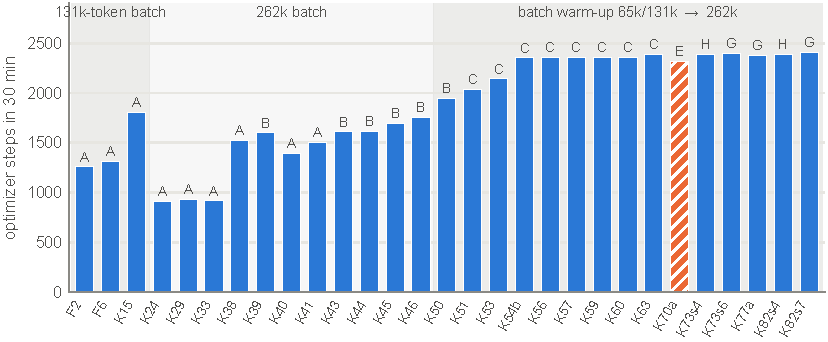
\includegraphics{step_counts.pdf}
  \caption{\textbf{Optimizer steps in the 30-minute budget}, from the rehearsal of each upload (cold, but warm for
    \upl{K15} and \upl{K38}); the letter is the chip. Shading marks the batch regime: a 131k-token batch before
    \upl{K24}, a constant 262k batch from \upl{K24}, and from \upl{K50} a batch warm-up through 65k and 131k phases,
    which adds steps early in the run.
    Step counts are comparable only within a regime and within a chip; hatched bars are chip~E, which ran slow.}
  \label{fig:steps}
\end{figure}

\clearpage
\section{Oracle details}
\label{app:oracle}

\begin{table}[!htbp]
  \centering
  \caption{\textbf{Offset $=$ official $-$ rehearsal, by period} ($10^{-3}$ bpb). The 95\% CI is the half-width for
    the mean (Student $t$). Ranges are rounded half-up from the exact differences. Official scores are published to
    four decimals, so every offset carries a rounding error of up to $\pm$\val{official-rounding}.}
  \label{tab:offset-periods}
  % GENERATED by paper/analysis -- offset = official - rehearsal by period, 1e-3 bpb (oracle.py)
{\small
\begin{tabular}{@{}p{5.6cm}rrrrr@{}}
\toprule
Uploads & $n$ & Mean & SD & Range & 95\% CI \\
\midrule
chip-C calibration uploads, K51--K60 & 7 & \ensuremath{+}6.53 & 0.42 & \ensuremath{+}6.1 to \ensuremath{+}7.2 & $\pm$0.39 \\
final day, chips C/E/G/H, K63--K82s7 & 7 & \ensuremath{+}6.87 & 0.30 & \ensuremath{+}6.5 to \ensuremath{+}7.4 & $\pm$0.27 \\
since K50 (all chips) & 15 & \ensuremath{+}6.71 & 0.38 & \ensuremath{+}6.1 to \ensuremath{+}7.4 & $\pm$0.21 \\
early, chips A/B, F2--K46 & 15 & \ensuremath{+}6.26 & 0.72 & \ensuremath{+}5.3 to \ensuremath{+}7.8 & $\pm$0.40 \\
every rehearsed upload & 30 & \ensuremath{+}6.48 & 0.61 & \ensuremath{+}5.3 to \ensuremath{+}7.8 & $\pm$0.23 \\
\bottomrule
\end{tabular}
}

\end{table}

\begin{table}[!htbp]
  \centering
  \caption{\textbf{Coverage of the expanding-window prediction intervals}: uploads inside the interval, with the
    expected count in brackets, for two burn-in lengths (\cref{sec:oracle-holdout}).}
  \label{tab:coverage}
  % GENERATED by paper/analysis -- observed (expected) count of uploads inside the expanding-window interval (oracle.py)
{\small
\begin{tabular}{@{}lcc@{}}
\toprule
Nominal level & Burn-in 3 uploads & Burn-in 5 uploads \\
\midrule
50\% & 7/12 (6.0) & 6/10 (5.0) \\
80\% & 11/12 (9.6) & 9/10 (8.0) \\
95\% & 12/12 (11.4) & 10/10 (9.5) \\
\bottomrule
\end{tabular}
}

\end{table}

\begin{table}[!htbp]
  \centering
  \caption{\textbf{Sensitivity of the oracle statistics to \upl{K70a}} ($10^{-3}$ bpb). ``Frozen'': the chip-C
    calibration on the final-day uploads. ``In 95\% PI'' and ``Seq.\ MAE'': the expanding window with a burn-in of
    three uploads.}
  \label{tab:oracle-sens}
  % GENERATED by paper/analysis -- oracle statistics with K70a as used, raw and excluded, 1e-3 bpb (oracle.py)
{\footnotesize
\begin{tabular}{@{}p{4.9cm}rrrrrrr@{}}
\toprule
Data since K50 & $n$ & Mean & SD & Frozen MAE & Frozen bias & In 95\% PI & Seq.\ MAE \\
\midrule
K70a normalised to chip-C speed (as used) & 15 & \ensuremath{+}6.71 & 0.38 & 0.35 & \ensuremath{+}0.34 & 12/12 & 0.31 \\
K70a raw chip-E rehearsal & 15 & \ensuremath{+}6.62 & 0.54 & 0.53 & \ensuremath{+}0.15 & 11/12 & 0.47 \\
K70a excluded & 14 & \ensuremath{+}6.72 & 0.39 & 0.40 & \ensuremath{+}0.39 & 11/11 & 0.34 \\
\bottomrule
\end{tabular}
}

\end{table}

\subsection{What the offset variance is made of}
\label{app:offset-detail}

Since \upl{K50} the within-chip offset SD is \val{off-sd-within}. If the official text behaves like the first 20M public tokens, the run-to-run variation of
the text gap (SD \val{offdec-text}) explains only \val{offdec-text-share} of the within-chip offset variance and
rounding to four decimals almost none (SD \val{offdec-round}); the remaining SD, \val{offdec-rest}
(\val{offdec-rest-lo}--\val{offdec-rest-hi} at the limits of the within-chip SD's interval), comes from step-count
jitter, from the official side or from nondeterminism, which these data cannot separate.

\paragraph{Chip or model quality?} On the final day the faster chips also rehearsed the better recipes and the
lottery winners, so an apparent chip effect could be an effect of model quality or of selection. Across the
\val{cq-n} uploads since \upl{K50}, the offset's slope on the rehearsal score is \val{cq-slope} (95\% CI
\val{cq-slope-lo} to \val{cq-slope-hi}, $p=\val{cq-slope-p}$), which moves the offset by \val{cq-slope-span} across
the rehearsal span. The \val{cq-gh-n} uploads rehearsed on chips G and H have a mean offset \val{cq-gh-diff} above the
rest (exact permutation $p=\val{cq-perm-p}$ over all \val{cq-perm-n} label assignments), but given the rehearsal score
the G/H term is \val{cq-gh-coef} (95\% CI \val{cq-gh-lo} to \val{cq-gh-hi}; permutation $p=\val{cq-perm-p-adj}$) and
the slope becomes \val{cq-slope-adj}. With so few uploads the data cannot tell a chip effect from an effect of model
quality or selection, so we say only that the offset \emph{may} depend on the chip.

\subsection{Traps in detail}
\label{app:traps}

The four ways in which a rehearsal was not a faithful replica of the official run (\cref{sec:traps}):
\begin{enumerate}
  \item \textbf{Cold means cold.} Any one-time compilation that happens after the clock starts costs steps in the
    official run. A warm rehearsal, which reuses compiled graphs, does not pay that cost. \Cref{sec:prewarm}
    quantifies one instance: warm rehearsals of an EMA recipe looked \val{ema-warm-bias}\docnum{} bpb better than the
    cold official run would be.
  \item \textbf{Chip speed.} A rehearsal predicts the official score only if the official host runs at the
    rehearsal chip's speed; otherwise $\gamma_c\neq0$. We normalised same-recipe runs to chip-C speed at $\rho$ and
    never across a change that alters step time.
  \item \textbf{The warm-up coin flip.} A change that touches steps 0--19 can move a seed onto a different early
    trajectory (\cref{sec:seeds}). The rehearsal still predicts the official score, because the official run takes
    the same path, but the measured difference is then a seed effect rather than the change's effect.
  \item \textbf{The time target is a budget, not a promise.} The training clock stops when the next step would
    cross the target; the median reserve was \val{reserve-s}\docnum{}~s over \val{reserve-n} completed runs, and we
    kept \val{headroom}\docnum{}~s of headroom under the cap.
\end{enumerate}
Two scores from runs that the organisers rescored, one each for \upl{K44} and \upl{F6}, are excluded from all
calibration statistics, so that each upload counts once; both are listed in
\path{research/sim-data/official-uploads.csv}.

\subsection{The normalised rehearsal of \upl{K70a}}
\label{sec:k70a}

Chip~E ran about \val{chip-spread}\docnum{} slower in step time than chip~C. \upl{K70a}'s raw chip-E rehearsal,
\val{k70a-raw}, was converted to chip-C speed by subtracting $\rho$ times its step deficit, which gave
\val{k70a-norm}: an adjustment of \val{k70a-adj}, i.e.\ \val{k70a-adj-pct} of steps at $\rho$ (not all of a
step-time deficit becomes a step deficit, because the schedule is clock-keyed). Its raw offset would be
\val{k70a-raw-offset}, an outlier. The repository does not show whether the normalised value was computed before the
upload: no time-stamped projection exists, so we treat it as a post-hoc adjustment. \Cref{tab:oracle-sens} gives
every oracle statistic three ways. With the raw rehearsal the since-\upl{K50} SD rises from \val{sens-used-sd} to
\val{sens-raw-sd}, the frozen MAE from \val{sens-used-mae} to \val{sens-raw-mae}, and the expanding-window count
falls to \val{sens-raw-inside}; excluding \upl{K70a} changes little.

\subsection{Expanding-window prediction}

\Cref{fig:offset-prospective} predicts each upload from the mean offset of all earlier uploads since \upl{K50}, with
a $t$ prediction interval, starting once three earlier points exist (\cref{sec:oracle-holdout}). \Cref{tab:coverage}
reports coverage at 50, 80 and 95\% for burn-ins of three and five uploads: at 50\% the intervals cover
\val{cov-50-b3} and \val{cov-50-b5}, close to nominal, and at 80\% \val{cov-80-b3} and \val{cov-80-b5}, slightly
conservative.

\begin{figure}[!htbp]
  \centering
  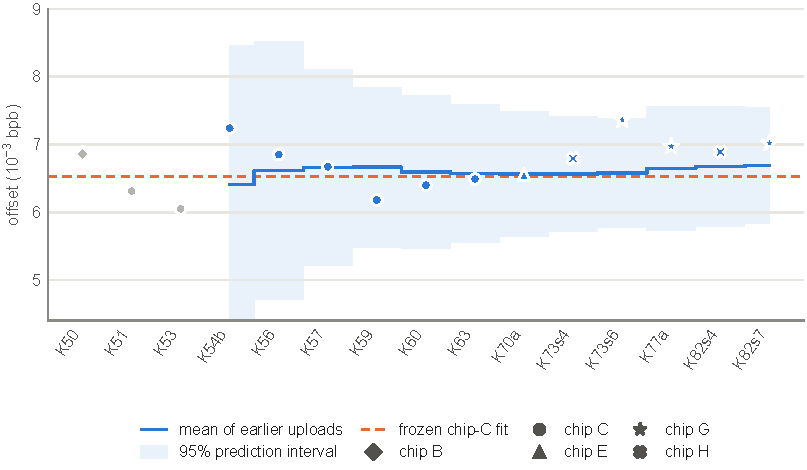
\includegraphics{offset_prospective.pdf}
  \caption{\textbf{Pseudo-prospective offset prediction.} Each point is an upload's offset (marker: rehearsal chip;
    grey: the three burn-in uploads). The solid line is the mean offset of all earlier uploads since \upl{K50}, the
    band its 95\% prediction interval, and the dashed line the frozen chip-C fit. Generated by
    \texttt{paper/analysis/oracle.py}.}
  \label{fig:offset-prospective}
\end{figure}

\subsection{The written projections}
\label{sec:projections}

The repository records three projections written before upload (\texttt{results/official-scores.csv},
\texttt{docs/EXACT-ORACLE.md}). \upl{K73s6} was projected at \val{k73s6-projected}\docnum{} and scored
\val{official-k73s6}, the largest miss (\val{k73s6-miss}). \upl{K82s4} was projected at
\val{k82s4-projected}\docnum{} and scored \val{best-official}; \upl{K82s7} was projected at about \val{k82s7-projected}\docnum{} and
scored \val{salt7-official}. These two projections did \emph{not} use the frozen chip-C offset, which misses them by
\val{ferr-k82s4} and \val{ferr-k82s7} (\cref{tab:offset-holdout}). They added an offset of \val{k82-proj-offset}\docnum{}
read off the final-day uploads already scored, most of them on the faster chips G and H; the exact rule was not
recorded. That is the text-plus-chip correction applied informally, which may be why those two landed close. It is
also a reason to treat their closeness as anecdote rather than as a test.

\section{Simulator internals}
\label{app:sim}

\subsection{Dataset}
\label{app:simdata}

Each record of \texttt{runs.jsonl} carries the effective \texttt{FF\_*} environment, steps, charged and start-up
seconds, median step time per accumulation phase, the early loss curve where logged (\val{ds-loss-curves} records),
and the \valbpb{} on the first 2M public tokens. Records outside the quality fit are screens, runs from the earliest
chips without a recorded code version, rows whose base recipe is unknown, or runs without a final score. The pairs
of \texttt{validation-pairs.json} pair each treatment with the control the campaign named at the time, leaving out
60-step screens\docnum{}; no earlier comparisons were paired.

\begin{table}[!htbp]
  \centering
  \caption{\textbf{Run records by instance} (\texttt{research/sim-data/runs.jsonl}). Chips A and B are the early
    instances whose records come from a run table without a code version; chip D ran an older Neuron runtime
    (2.33.10, against 2.34.10 on chip C). ``Unknown'': records without a recorded chip. The final-day chips E, G and
    H are not in the dataset.}
  \label{tab:dataset}
  % GENERATED by paper/analysis -- runs.jsonl by chip (simulator.py)
{\small
\begin{tabular}{@{}lrrrrr@{}}
\toprule
Chip & Records & Full runs & Screens & Full, with bpb & Loss curves \\
\midrule
unknown & 28 & 28 & 0 & 5 & 0 \\
A & 563 & 426 & 137 & 390 & 0 \\
B & 247 & 234 & 13 & 220 & 0 \\
C & 349 & 223 & 126 & 215 & 331 \\
D & 19 & 17 & 2 & 17 & 11 \\
\midrule
all & 1{,}206 & 928 & 278 & 847 & 342 \\
\bottomrule
\end{tabular}
}

\end{table}

\subsection{Step time and the step walk}
\label{app:steptime}

The step-time model regresses the median $k\!=\!1,2,4$ step times on code-lineage effects and knob features (depth,
width, batch, fused paths). It is deliberately empirical, because the Neuron compiler is far from linear in
operation count: removing one elementwise pass over the MLP activation saved \val{st-onepass}\docnum{}, fusing the
QKV projection, which has fewer operations, was \val{st-qkv}\docnum{} \emph{slower}, and a 96-parameter gate cost
\val{st-gate}\docnum{}. A mechanism that no fitted run carries is charged a \val{st-novel-prior}\docnum{} prior and
flagged ``cost unknown''. Medians are scaled by the measured median-to-mean overhead (\val{overhead}) before the walk.
With one code lineage left out, the model predicts the $k\!=\!4$ step time of runs whose mechanisms another lineage
carried, with an MAE of \val{st-lolo-reach} (\val{st-lolo-nreach} runs; \cref{tab:sim-other}), and the walk reproduces
a rehearsal's phase switches to within \val{walk-phase-err}\docnum{} steps.

\subsection{Features and code eras}

The quality surrogate reads \val{q-nbase-features} base features (\cref{tab:features}) and \val{q-nbowl-features}
non-negative curvature (``bowl'') terms for tuned scalars, the squares of the corresponding base features. Every
feature is centred on the \upl{K59} reference recipe, so the era intercept of the current code family is that recipe's
predicted score at 2{,}300 steps on chip~C. Each feature's scale in \cref{tab:features} is the size of a typical campaign move; the ridge prior applies
per scaled unit. \emph{Code eras} are groups of versions of our training script: M3 to M14 number the main lineage in
order, and ``M9+'' groups the flag-gated versions from M9 on, whose new mechanisms are off unless a knob turns them on.

\begin{table}[!htbp]
  \centering
  \caption{\textbf{Knob features of the quality surrogate} (\texttt{ffsim/quality.py}, \texttt{FEATURES}). Two
encodings were set with campaign outcomes in view: the \texttt{leaky\_sq} bowl, centred on the slope 0.35 that had
measured best, and \texttt{acc\_in\_graph}, added after the \upl{K56} mechanism had measured well.}
  \label{tab:features}
  % GENERATED by paper/analysis -- ffsim.quality FEATURES (simulator.py)
{\scriptsize
\begin{tabular}{@{}lp{10.6cm}r@{}}
\toprule
Feature & Encoding (centred on the K59 recipe) & Scale \\
\midrule
\texttt{leaky} & LK - 0.35 (leaky relu\textsuperscript{2} slope; 0 = plain relu\textsuperscript{2}) & 0.15 \\
\texttt{leaky\_sq} & (LK - 0.35)\textsuperscript{2}: a bowl in the slope (0 / 0.25 / 0.35 / 0.5 were tried) & 0.0225 \\
\texttt{leaky\_form\_abs} & 1 if LK > 0 and form is 'abs' (M10b); fn/fnm = 0 & 1 \\
\texttt{leaky\_form\_max} & 1 if LK > 0 and form is 'max' (M11c, torch.maximum) & 1 \\
\texttt{relu2\_fn} & 1 if FF\_RELU2\_FN (the RF arm: relu\textsuperscript{2} with a hand-written backward, LK = 0) & 1 \\
\texttt{softcap\_log} & ln(SOFTCAP / 15) when SOFTCAP > 0, else 0 & 0.182 \\
\texttt{softcap\_off} & 1 if SOFTCAP == 0 (no logit cap) & 1 \\
\texttt{softcap\_a} & A\_eff / SOFTCAP - 1 with A\_eff = SOFTCAP\_A if > 0 else SOFTCAP (asymmetric cap A*tanh(z/C): 16.5 on 15 $\rightarrow$ 0.1) & 0.1 \\
\texttt{softcap\_b} & SOFTCAP\_B (logit shift inside the tanh) & 5 \\
\texttt{wd\_sched} & WD\_SCHED power (muon wd = WD * lrm ** WD\_SCHED; 0 = constant wd; non-numeric $\rightarrow$ 1) & 1 \\
\texttt{mom\_peak} & MOM\_PEAK - 0.95 (Muon momentum peak; 0.93 / 0.97 were tried) & 0.02 \\
\texttt{muon\_beta2} & MUON\_BETA2 - 0.9 (0.8 and 0.98 were tried) & 0.05 \\
\texttt{rope\_log} & ln(ROPE\_BASE / 1e5) (300k tried) & 1.1 \\
\texttt{scalar\_beta2} & SCALAR\_BETA2 - 0.95 (0.99 tried) & 0.04 \\
\texttt{qk\_gain} & QK\_GAIN - 1.44 (1.6 tried) & 0.16 \\
\texttt{warmup\_log} & ln(WARMUP / 20) (40 tried) & 0.693 \\
\texttt{emb\_lr\_log} & ln(EMB\_LR / 0.30) (0.36 tried) & 0.182 \\
\texttt{unemb\_lr\_log} & ln(UNEMB\_LR / 0.006) (0.0072 tried) & 0.182 \\
\texttt{scalar\_lr\_log} & ln(SCALAR\_LR / 0.20) (0.1664 tried with ADAMW\_LR 1.7) & 0.182 \\
\texttt{matrix\_lr\_log} & ln(MATRIX\_LR\_SCALE / 2.0) (1.75 / 2.3 tried) & 0.14 \\
\texttt{adamw\_lr\_log} & ln(ADAMW\_LR\_SCALE / 1.4142) (1.7 tried) & 0.182 \\
\texttt{wd\_log} & ln(WD / 0.02) (0.012 / 0.03 tried) & 0.405 \\
\texttt{key\_offset\_off} & 1 if the rotary key offset is off (pre-K51 recipes) & 1 \\
\texttt{key\_offset\_log} & ln(radius / 0.3) when the key offset is on (0.03 / 0.1 / 0.2 / 0.5 / 1.0 / 3.0 were tried: two decades, so a log scale), 0 when off & 1.1 \\
\texttt{acc\_in\_graph} & ACC\_IN\_GRAPH - 1 (K56 mechanism: gradient accumulation inside the compiled graph) & 1 \\
\texttt{accum\_until} & charged-time fraction at which the batch warm-up reaches the final k, minus 0.2 (plain 'K' $\rightarrow$ -0.2; '2:0.2,4' and RAMP3 $\rightarrow$ 0) & 0.2 \\
\texttt{accum\_k1\_until} & first-phase (k1) end fraction minus 0.06 (RAMP3 $\rightarrow$ 0; two-phase or none $\rightarrow$ -0.06) & 0.06 \\
\texttt{accum\_lr0} & LR scale of the first small-batch phase minus 0.5 (0 when no batch warm-up) & 0.25 \\
\texttt{accum\_lr1} & LR scale of the second small-batch phase minus 0.7071 (0 unless RAMP3) & 0.25 \\
\texttt{cooldown\_frac} & COOLDOWN\_FRAC - 0.6 (0.45 / 0.55 / 0.65 tried) & 0.1 \\
\texttt{mtp\_off} & 1 if FF\_MTP == 0 (no multi-token head) & 1 \\
\texttt{mtp\_p1} & MTP fade phase 1 - 0.2 (0 when MTP off) & 0.1 \\
\texttt{mtp\_p2} & MTP fade phase 2 - 0.45 (0 when MTP off; 0.5 tried) & 0.1 \\
\texttt{mtp\_w\_tail} & sum of the MTP head weights after the first, minus 0.75 ('1,0.6,0.3' $\rightarrow$ 0.15; 0 when MTP off) & 0.15 \\
\texttt{xsa\_on} & 1 if FF\_XSA\_LAYERS is non-empty & 1 \\
\texttt{xsa\_frac} & fraction of blocks with XSA ('all' $\rightarrow$ 1; '0,1,2,3' on d9 $\rightarrow$ 0.44) & 1 \\
\texttt{attn\_src} & 1 if FF\_ATTN\_SRC is non-empty (attention-source reuse, M14 '5:6,7,8') & 1 \\
\texttt{fn\_flags} & fraction of the M13 autograd.Function flags on (step-time mechanisms, quality-neutral by design: prior sd 0.001) & 1 \\
\texttt{ce\_bf16} & 1 if the cross-entropy runs in bf16 (G3 probe, rejected) & 1 \\
\texttt{ptp\_w} & PTP\_W (previous-token-prediction head weight; 0.25 tried) & 0.25 \\
\texttt{mom\_ramp\_log} & ln(MOM\_RAMP / 300) (450 tried) & 0.405 \\
\texttt{depth} & DEPTH - 9 (8 / 10 / 12 tried) & 1 \\
\texttt{aspect\_log} & ln(ASPECT\_RATIO / 113) (width = aspect * depth) & 0.0953 \\
\texttt{total\_batch\_log2} & log2(TOTAL\_BATCH / 262144) & 1 \\
\texttt{mlp\_mult} & MLP\_MULT - 4 & 1 \\
\texttt{time\_target\_log} & ln(TIME\_TARGET / 1793): mostly absorbed by ln(steps), so its prior sd is 0.001 and it only catches what the step count misses & 0.0953 \\
\bottomrule
\end{tabular}
}

\end{table}

\subsection{Fitting the quality surrogate}
\label{app:fit}

The fit of \cref{eq:quality} is not one closed-form solve. For a given residual SD $\sigma_q$, the MAP estimate solves
$(X^\top X + \sigma_q^2 D)\hat\beta = X^\top y + \sigma_q^2 D m$ with $D=\mathrm{diag}(1/s_j^2)$ for prior SDs $s_j$
and prior means $m$. A bowl coefficient that comes out negative is pinned at zero and the system re-solved (an
active-set solution of the non-negativity constraint). $\sigma_q$ is then re-estimated by empirical Bayes from the
residuals and effective degrees of freedom, three times, and floored at \val{q-sigma-floor}. Seed effects are
estimated jointly, as best linear unbiased predictors. The fit uses \val{q-nfit} runs, \val{q-ncols} columns and
\val{q-neras} eras, with \val{q-edf} effective degrees of freedom.

\paragraph{Paired Monte Carlo.} \texttt{simulate} and \texttt{search} propagate chip jitter, seed luck, coefficient
uncertainty, residuals and the offset by Monte Carlo with common random numbers, so that wherever two recipes agree
the noise cancels. $P(\text{candidate} < \text{base})$ is a paired probability; we have not checked its calibration
beyond interval coverage (\val{lopo-rec-cover} of LOPO recipe pairs fall inside the predicted $\pm2$\,SD,
\cref{sec:simval}). An identical recipe reproduces the base exactly.

\subsection{What the surrogate learned}

\Cref{tab:coefficients} lists the knob coefficients furthest from zero in posterior-SD units. Read it with the
support columns. A feature varied in a single run (\texttt{ce\_bf16}, \texttt{accum\_lr1}) or only inside early eras
(\texttt{key\_offset\_off}, varied only in M3 and M4) is identified mostly by those runs and partly absorbs era
differences. Such coefficients are bookkeeping for prediction, not causal effect sizes. The attention-source
coefficient (\texttt{attn\_src}) rests on two runs, which is why the post-fit attention-source pairs were
over-predicted (\cref{tab:postfit}).

\begin{table}[!htbp]
  \centering
  \caption{\textbf{The \val{coef-ntop} knob coefficients furthest from zero} in posterior-SD units, in $10^{-3}$ bpb
    per scaled unit. ``Runs $\neq0$'' counts fitted runs in which the feature is non-zero, and ``Code eras'' the eras
    those runs come from. Knob names omit the \texttt{FF\_} prefix.}
  \label{tab:coefficients}
  % GENERATED by paper/analysis -- the 16 knob coefficients furthest from zero in posterior-SD units, x 1e-3 bpb per scaled unit
{\footnotesize\setlength{\tabcolsep}{4pt}
\begin{tabular}{@{}lp{3.6cm}rrrrp{2.6cm}@{}}
\toprule
Feature & Knob(s) & Est. & Post.\ SD & Prior SD & Runs $\neq0$ & Code eras \\
\midrule
\texttt{accum\_until} & ACCUM\_SCHED & \ensuremath{+}6.37 & 0.60 & 4.0 & 10 & M3, M6, M7 \\
\texttt{ce\_bf16} & CE\_BF16 & \ensuremath{+}2.93 & 0.34 & 4.0 & 1 & M6 \\
\texttt{attn\_src} & ATTN\_SRC & \ensuremath{-}2.02 & 0.25 & 4.0 & 2 & M9+ \\
\texttt{accum\_lr0} & ACCUM\_LR, ACCUM\_SCHED & \ensuremath{-}2.42 & 0.44 & 4.0 & 34 & M3, M4, M5, M6, M7 \\
\texttt{key\_offset\_log\_sq} & KEY\_OFFSET\_RAD, KEY\_OFFSET & \ensuremath{+}0.46 & 0.10 & 1.0 & 48 & M4, M5, M6, M7 \\
\texttt{leaky\_sq} & LEAKY\_RELU2 & \ensuremath{+}0.28 & 0.06 & 1.0 & 111 & M3, M4, M5, M6, M7, M9+ \\
\texttt{mom\_peak\_sq} & MOM\_PEAK & \ensuremath{+}1.09 & 0.24 & 1.0 & 2 & M9+ \\
\texttt{mom\_peak} & MOM\_PEAK & \ensuremath{+}0.74 & 0.21 & 4.0 & 2 & M9+ \\
\texttt{key\_offset\_off} & KEY\_OFFSET & \ensuremath{-}4.75 & 1.41 & 4.0 & 8 & M3, M4 \\
\texttt{accum\_k1\_until} & ACCUM\_SCHED & \ensuremath{+}0.90 & 0.34 & 4.0 & 35 & M3, M4, M5, M6, M7 \\
\texttt{accum\_lr1} & ACCUM\_LR, ACCUM\_SCHED & \ensuremath{+}2.43 & 0.94 & 4.0 & 1 & M7 \\
\texttt{xsa\_frac} & XSA\_LAYERS, DEPTH & \ensuremath{-}1.84 & 0.86 & 4.0 & 2 & M9+ \\
\texttt{leaky} & LEAKY\_RELU2 & \ensuremath{+}0.18 & 0.11 & 4.0 & 111 & M3, M4, M5, M6, M7, M9+ \\
\texttt{softcap\_a} & SOFTCAP\_A, SOFTCAP & \ensuremath{-}0.29 & 0.20 & 4.0 & 4 & M5, M9+ \\
\texttt{mom\_ramp\_log} & MOM\_RAMP & \ensuremath{+}0.35 & 0.42 & 4.0 & 2 & M5 \\
\texttt{matrix\_lr\_log} & MATRIX\_LR\_SCALE & \ensuremath{+}0.18 & 0.22 & 4.0 & 2 & M7 \\
\bottomrule
\end{tabular}
}

\end{table}

\subsection{Pair validation by family, forward in time, and on new mechanisms}
\label{app:pairval}

Against the family-mean baseline, which scores \val{base-fam-rec-sign} (\val{base-fam-rec-signci}) with MAE
\val{base-fam-rec-mae} on the recipe pairs, the surrogate's MAE difference, \val{base-diff-fam-mae-ci}$\times10^{-3}$,
includes zero. ``Decisive'' pairs defined by the measured outcome ($|\Delta|\ge0.0003$) favour large step-count changes, so
\cref{sec:simval} reports the pairs on which the \emph{prediction} is decisive; on them the MAE is
\val{base-full-pdec-mae} for the surrogate against \val{base-steps-pdec-mae} for the steps-only model. Forward in
time, the surrogate's MAE is better than the steps-only model's with the 29~September cutoff (difference
\val{temp-b-diff-mae-ci}$\times10^{-3}$) but not with 28~September (\val{temp-a-diff-mae-ci}$\times10^{-3}$), where the zero
predictor's MAE is \val{temp-a-zero-mae}. During development (\cref{tab:surrogate-configs}), a fix to how missing
knobs are read moved LOPO sign agreement on the pairs named in the simulator's specification from
\val{sc-spec-sign-before}\docnum{} to \val{sc-spec-sign-after}\docnum{}, and recipe-pair sign agreement ranged from
\val{sc-rec-sign-lo}\docnum{} (\val{sc-rec-lo-name}) to \val{sc-rec-sign-hi}\docnum{} (\val{sc-rec-hi-name}) across
configurations; the default, \val{sc-default-name}, scored \val{sc-default-rec-sign}\docnum{}.

\begin{table}[!htbp]
  \centering
  \caption{\textbf{Leave one pair out (LOPO) and leave one knob value out (LOKVO) by pair family}, in $10^{-3}$ bpb.
    The ``seed'' and ``chip'' families compare identical recipes and measure noise; ``cold upload rehearsals'' pairs
    compare upload rehearsals.}
  \label{tab:lopo-family}
  % GENERATED by paper/analysis -- per-family pair validation, 1e-3 bpb (simulator.py)
{\footnotesize
\begin{tabular}{@{}p{4.4cm}rrrrrr@{}}
\toprule
Pair family & $n$ & Mean $\Delta$ & LOPO sign & LOPO MAE & LOKVO sign & LOKVO MAE \\
\midrule
LeakyReLU slope & 13 & \ensuremath{-}0.83 & 92\% & 0.33 & 69\% & 0.82 \\
seed (noise) & 11 & \ensuremath{+}1.43 & 100\% & 0.59 & 100\% & 0.59 \\
scalar retunes, K57 base & 10 & \ensuremath{+}0.28 & 70\% & 0.71 & 70\% & 0.73 \\
batch warm-up schedule & 9 & \ensuremath{-}0.23 & 89\% & 0.17 & 89\% & 0.23 \\
cold upload rehearsals & 9 & \ensuremath{-}0.64 & 67\% & 0.27 & 78\% & 0.96 \\
LeakyReLU form & 8 & \ensuremath{+}0.03 & 88\% & 0.41 & 88\% & 0.99 \\
key-offset radius & 7 & \ensuremath{-}0.20 & 100\% & 0.20 & 100\% & 0.19 \\
weight-decay schedule & 4 & \ensuremath{-}0.03 & 75\% & 0.08 & 75\% & 0.07 \\
accumulation in graph & 3 & \ensuremath{-}0.61 & 100\% & 0.06 & 100\% & 0.08 \\
QK gain & 3 & \ensuremath{+}0.08 & 33\% & 0.59 & 33\% & 0.54 \\
ReLU$^2$ hand-written backward & 3 & \ensuremath{-}1.12 & 100\% & 0.16 & 100\% & 0.10 \\
AdamW $\beta_2$ & 2 & \ensuremath{+}0.39 & 100\% & 0.96 & 100\% & 0.96 \\
learning rate & 2 & \ensuremath{+}0.18 & 100\% & 0.45 & 100\% & 0.45 \\
Muon momentum peak & 2 & \ensuremath{+}1.26 & 50\% & 1.21 & 50\% & 1.21 \\
asymmetric soft cap & 2 & \ensuremath{-}0.08 & 50\% & 0.17 & 100\% & 0.11 \\
attention-input shift & 2 & \ensuremath{+}2.30 & 100\% & 0.77 & 100\% & 0.77 \\
ZeRO-2 + AdamW ZeRO & 2 & \ensuremath{-}1.39 & 100\% & 0.19 & 100\% & 0.19 \\
chip (noise) & 1 & \ensuremath{+}4.68 & 100\% & 0.39 & 100\% & 0.39 \\
code-M13 flags & 1 & \ensuremath{+}0.06 & 0\% & 0.32 & 0\% & 0.32 \\
attention-source reuse & 1 & \ensuremath{-}1.73 & 100\% & 0.42 & 100\% & 1.68 \\
multi-token prediction & 1 & \ensuremath{+}0.06 & 100\% & 0.04 & 100\% & 0.04 \\
RoPE base & 1 & \ensuremath{+}0.15 & 100\% & 0.17 & 100\% & 0.17 \\
soft cap & 1 & \ensuremath{+}0.35 & 100\% & 0.08 & 100\% & 0.08 \\
LR warm-up & 1 & \ensuremath{+}0.66 & 100\% & 0.68 & 100\% & 0.68 \\
\bottomrule
\end{tabular}
}

\end{table}

\begin{figure}[!htbp]
  \centering
  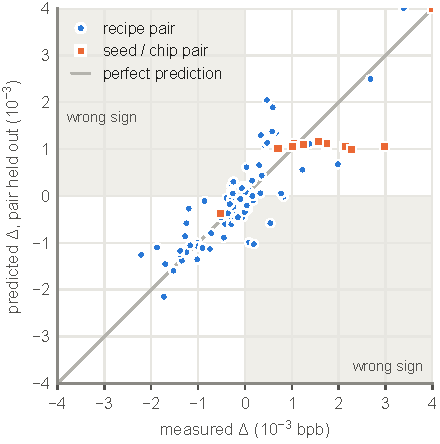
\includegraphics{simulator_pairs.pdf}
  \caption{\textbf{The quality surrogate on pairs it did not see} (leave one pair out, all \val{lopo-all-n} pairs;
    values beyond $\pm4\times10^{-3}$ are drawn at the edge). Shaded quadrants mark a wrong predicted sign. Squares
    are seed and chip pairs, which measure run-to-run noise rather than a recipe effect.}
  \label{fig:pairs}
\end{figure}

\begin{table}[!htbp]
  \centering
  \caption{\textbf{Temporal hold-out of the quality surrogate.} ``Supported'' pairs move only features that some run
    in the restricted fit varied; ``Prior-only'' pairs move a feature that no such run varied, so the model can only
    return its prior for it. Cells in these two columns give $n$: sign agreement of the surrogate. ``Steps only'': the same model
    with every knob effect switched off, fitted on the same early runs; ``Zero'': the predictor $\hat\Delta=0$.}
  \label{tab:temporal}
  % GENERATED by paper/analysis -- temporal hold-out (simulator.py); MAE in 1e-3 bpb; supported / prior-only cells are n: sign agreement
{\footnotesize\setlength{\tabcolsep}{4pt}
\begin{tabular}{@{}lrrrrrrrrr@{}}
\toprule
MAE in $10^{-3}$ bpb & & & \multicolumn{2}{c}{Surrogate} & \multicolumn{2}{c}{Steps only} & Zero & & \\
\cmidrule(lr){4-5}\cmidrule(lr){6-7}
Fit on & Runs & Pairs & Sign & MAE & Sign & MAE & MAE & Supported & Prior-only \\
\midrule
runs before 28 Sep & 59 & 72 & 86\% & 0.89 & 71\% & 0.78 & 0.94 & 36: 89\% & 36: 83\% \\
runs before 29 Sep & 98 & 46 & 91\% & 0.48 & 67\% & 0.89 & 1.08 & 32: 91\% & 14: 93\% \\
\bottomrule
\end{tabular}
}

\end{table}

With the 28~September cutoff, the \val{temp-a-sup-n} temporal pairs whose moved features the restricted fit had
seen score \val{temp-a-sup-sign}, and the \val{temp-a-uns-n} pairs that only the prior can answer score
\val{temp-a-uns-sign}; with 29~September the two groups score \val{temp-b-sup-sign} and \val{temp-b-uns-sign}
(\cref{tab:temporal}). For the prior-only pairs the sign must come from the step term, the era and seed effects and
the positive prior means of the bowl terms, which make a move away from a tuned value cost (\cref{app:fit}).

\begin{table}[!htbp]
  \centering
  \caption{\textbf{The \val{postfit-n} pairs that finished after the release fit} ($10^{-3}$ bpb). Observed and
    predicted values per pair are from \texttt{docs/simulator-report-20260929.md} \S5\docnum{} (the model was the
    release fit, in the candidate convention); sign agreement, the Wilson interval and the MAE are computed by
    \texttt{paper/analysis/simulator.py}; the Wilson interval treats the pairs as independent, but several share a
    control, so it is too narrow. AS: attention-source variants; ALR: AdamW learning-rate change.}
  \label{tab:postfit}
  % GENERATED by paper/analysis -- 15 post-fit pairs, 1e-3 bpb (simulator.py)
{\footnotesize
\begin{tabular}{@{}p{6.4cm}rrc@{}}
\toprule
Pair (report label) & Observed & Predicted & Sign \\
\midrule
C41 K60 vs C40 K59 (cold rehearsals) & \ensuremath{-}1.82 & \ensuremath{-}2.10 & yes \\
AS-a s67 (C) & \ensuremath{-}1.36 & \ensuremath{-}2.04 & yes \\
AS-a s58 (C) & \ensuremath{-}1.06 & \ensuremath{-}1.71 & yes \\
AS-a s97 (D) & \ensuremath{+}1.15 & \ensuremath{-}0.99 & no \\
AS-b 4:5,6,7,8 s73 (D) & \ensuremath{-}0.86 & \ensuremath{-}2.29 & yes \\
K60 + ALR s73 (C) vs AS-a & \ensuremath{+}0.81 & \ensuremath{+}1.67 & yes \\
K60 + ALR s67 (C) vs AS-a & \ensuremath{+}0.95 & \ensuremath{+}2.24 & yes \\
ALR s97 (D) vs LK0.35 & \ensuremath{-}0.78 & \ensuremath{+}1.73 & no \\
ALR s113 (D) vs LK0.35 & \ensuremath{-}0.09 & \ensuremath{+}1.81 & no \\
ALR s131 (D) vs LK0.35 & \ensuremath{+}0.44 & \ensuremath{+}2.13 & yes \\
AS-d 5:7,8 s73 (C) vs AS-a & 0.00 & \ensuremath{+}0.15 & no \\
AS-d 5:7,8 s67 (C) vs AS-a & \ensuremath{+}0.33 & \ensuremath{+}0.39 & yes \\
AS-d 5:7,8 s73 (D) vs AS-a & \ensuremath{-}0.20 & \ensuremath{+}0.02 & no \\
AS-c 6:7,8 s73 (D) vs AS-a & \ensuremath{+}0.76 & \ensuremath{-}0.07 & no \\
K60 + softcap 16.5 s73 (C) vs AS-a & \ensuremath{+}0.68 & \ensuremath{-}0.22 & no \\
\midrule
sign agreement 8/15 (Wilson 95\%: 30\%--75\%) & & MAE 1.04 & \\
\bottomrule
\end{tabular}
}

\end{table}

\begin{table}[!htbp]
  \centering
  \caption{\textbf{Step-time model, end-to-end anchors and the offset model.} End-to-end rows compare the Monte Carlo
    prediction at seed~73 with the measured upload (\texttt{docs/SIMULATOR.md}\docnum{}).}
  \label{tab:sim-other}
  % GENERATED by paper/analysis -- step time, end-to-end anchors and the offset model (simulator.py); anchors from docs/SIMULATOR.md
{\footnotesize
\begin{tabular}{@{}p{6.2cm}rll@{}}
\toprule
Check & Data & Predicted & Measured / note \\
\midrule
Step time, k4 phase, leave one code lineage out: runs whose mechanisms another lineage ran & 161 runs & MAE 0.54\% & target 0.5\% \\
\quad all held-out runs, including novel mechanisms & 189 runs & MAE 0.95\% & up to 14\% \\
\midrule
End to end, \upl{K59}: steps / rehearsal / official$^{\dagger}$ & 1 upload & 2{,}369 / 0.96082 / 0.9674 & 2{,}357 / 0.96092 / 0.9671 \\
End to end, \upl{K60}: steps / rehearsal / official$^{\dagger}$ & 1 upload & 2{,}365 / 0.95888 / 0.9654 & 2{,}361 / 0.95910 / 0.9655 \\
\midrule
Offset model (chip-C uploads): mean and SD & 7 uploads & \ensuremath{+}0.00653, 0.00042 & SD 95\% CI 0.00027--0.00092 \\
\bottomrule
\end{tabular}
}

\end{table}

The full validation reports, including support grading for every knob value and the leakage guard, are
\texttt{research/sim-data/steptime-validation.md}, \texttt{simulate-validation.md} and \texttt{dataset-qa.md}.
\texttt{research/sim-data/quality-validation.md} is a historical report: it was written on an earlier snapshot of the
dataset (\val{qv-records}\docnum{} records), and the script that generated it is not released, so its numbers are
not recomputed here. Its \S11 compares the \val{sc-n}\docnum{} surrogate configurations of \cref{tab:surrogate-configs},
whose LOPO results were visible while the default was chosen (\cref{sec:simval}).

\begin{table}[!htbp]
  \centering
  \caption{\textbf{The surrogate configurations compared during development}, as printed in
    \texttt{research/sim-data/quality-validation.md} \S11\docnum{} (an earlier snapshot of the data; MAE in
    $10^{-3}$ bpb). The first LOPO and the LOKVO columns use the pairs named in the simulator's specification;
    ``recipe'' is the subset that changes the recipe, and ``Decisive'' its decisive pairs as defined in that report.
    The default configuration, in bold, is the one used throughout the paper.}
  \label{tab:surrogate-configs}
  % GENERATED by paper/analysis -- surrogate configurations, research/sim-data/quality-validation.md section 11 (values as printed there); MAE in 1e-3 bpb (simulator.py)
{\footnotesize\setlength{\tabcolsep}{4pt}
\begin{tabular}{@{}lp{4.2cm}rrrrrrrr@{}}
\toprule
& & & \multicolumn{2}{c}{LOPO, \val{sc-spec-n} pairs} & \multicolumn{2}{c}{LOPO, recipe} & Decisive & \multicolumn{2}{c}{LOKVO, \val{sc-spec-n} pairs} \\
\cmidrule(lr){4-5}\cmidrule(lr){6-7}\cmidrule(lr){9-10}
Config & Change & Runs & Sign & MAE & Sign & MAE & sign & Sign & MAE \\
\midrule
{A0} & original conventions: K59 defaults for missing knobs, no leakage guard, every code version its own era & 131 & 84\% & 0.66 & 81\% & 0.68 & 92\% & 71\% & 0.86 \\
{A1} & code defaults for missing knobs, code lineage, leakage guard & 131 & 85\% & 0.38 & 82\% & 0.34 & 92\% & 63\% & 0.87 \\
{A2} & A1 + one era for M9 and its flag-gated successors & 131 & 81\% & 0.38 & 77\% & 0.34 & 90\% & 70\% & 0.73 \\
\textbf{A3} & A2 + bowl prior on tuned knobs, bowls $\ge 0$ (the default) & 131 & 85\% & 0.38 & 82\% & 0.34 & 95\% & 84\% & 0.60 \\
{A4} & A3, slope prior SD 0.002 & 131 & 86\% & 0.38 & 84\% & 0.34 & 97\% & 84\% & 0.61 \\
{A5} & A3, seed prior SD 0.0009 & 131 & 85\% & 0.38 & 82\% & 0.34 & 95\% & 84\% & 0.69 \\
{A6} & A3, era grouping off & 131 & 90\% & 0.38 & 89\% & 0.34 & 97\% & 78\% & 0.73 \\
{A7} & A3, K59 defaults for missing knobs & 131 & 74\% & 0.66 & 69\% & 0.68 & 87\% & 70\% & 0.81 \\
{A8} & A3, bowl prior mean 0.001 & 131 & 86\% & 0.42 & 84\% & 0.39 & 97\% & 85\% & 0.69 \\
{A9} & A3, knob prior SD 0.002 & 131 & 85\% & 0.37 & 82\% & 0.33 & 95\% & 84\% & 0.64 \\
{A10} & A3 without the bowl constraint & 131 & 85\% & 0.38 & 82\% & 0.34 & 95\% & 84\% & 0.60 \\
{A11} & A3 fitted on M9+ runs only & 71 & 85\% & 0.65 & 82\% & 0.65 & 97\% & 82\% & 0.86 \\
\bottomrule
\end{tabular}
}

\end{table}

\section{Seed sweeps}

\begin{table}[!htbp]
  \centering
  \caption{\textbf{Warm-up paths in three seed sweeps of a fixed recipe} (full chip runs that differ only in the
    seed; $10^{-3}$ bpb). ``Spike'': step-10 loss $\ge$\val{spike-l10} nats; ``Interm.'': between \val{l10-interm-lo} and
    \val{spike-l10}. The difference is a Welch mean difference with 95\% CI. Generated by
    \texttt{paper/analysis/seeds.py}.}
  \label{tab:seeds}
  % GENERATED by paper/analysis -- warm-up path per seed sweep, 1e-3 bpb (seeds.py)
{\footnotesize\setlength{\tabcolsep}{4pt}
\begin{tabular}{@{}p{4.0cm}rrrrlrr@{}}
\toprule
Seed sweep & Seeds & Curve & Spike & Interm. & Spike $-$ good [95\% CI] & SD all & SD good \\
\midrule
K57 recipe (M9), chip C & 13 & 13 & 4 & 1 & \ensuremath{+}0.93 [\ensuremath{+}0.31, \ensuremath{+}1.56] & 0.61 & 0.42 \\
LeakyReLU(0.35)$^2$ (M12), chip C & 9 & 7 & 2 & 0 & \ensuremath{+}1.52 [\ensuremath{-}0.06, \ensuremath{+}3.10] & 1.32 & 0.53 \\
LeakyReLU(0.35)$^2$ (M12), chip D & 7 & 7 & 4 & 0 & \ensuremath{+}1.38 [0.00, \ensuremath{+}2.77] & 0.95 & 0.66 \\
\midrule
pooled (centred on each group's good-path mean) & 29 & 27 & 10 & & \ensuremath{+}1.23 [\ensuremath{+}0.80, \ensuremath{+}1.66] & & \\
\bottomrule
\end{tabular}
}

\end{table}

\clearpage
\section{The contribution pipeline}
\label{app:contrib}

\paragraph{The record.} One JSON object per run with a published schema: hardware, time budget, an optional
published base recipe (\upl{K82s4}, \upl{K60}, \upl{K59}) plus only the knobs that were changed, seed, steps, the
local rehearsal score and/or the official score, and an explicit consent flag. A run can be submitted through the
local app, a GitHub issue form or the command line; the app and the command line only \emph{build} a pre-filled issue
link and never send anything themselves.

\paragraph{Validation.} A schema check run by a small built-in interpreter; a scan for anything that looks like a
secret or personal data (access keys, account and resource identifiers, tokens, private keys, e-mail and host IP
addresses), with the field named but the value never repeated; plausible ranges for every knob the model reads,
rejection of non-finite numbers, and a finite feature vector and prediction; duplicate detection by a content hash;
and an outlier check against the current model, which flags a record with $|z|>\val{guard-outlier-z}$ for the
reviewer.

\paragraph{Entering the fit.} Each (hardware, base recipe) combination gets its own fixed effect with the same prior
as a chip. Runs shorter than \val{guard-min-steps} steps are stored but never fitted. A published base whose newest
levers lie outside the data (\upl{K82s4}) is anchored to its measured rehearsal (\val{guard-anchor}) until its effect
has data of its own.

\paragraph{Review and merge.} Only a label added by an account with write access approves a record, and editing the
issue afterwards removes the label. The approval opens a pull request that appends the record exactly as approved, on a
branch named by its content hash. Merging triggers a guarded refit whose output arrives as a second pull request;
nothing pushes to the main branch. Workflows run with read-only tokens wherever possible, pin every action to a commit
hash and never execute contributed content.

\paragraph{Stress test.} \Cref{tab:guard} pushes synthetic records through the real validation and guard code in
memory (\texttt{paper/analysis/contrib\_guard.py}). Honest records are the model's own prediction plus a hardware
bias and seed-sized noise, on knob values the data have seen; they moved the base predictions by at most
\val{guard-honest-c-shift} and were accepted. A single record 0.01~bpb worse than predicted was absorbed by its own
hardware effect (base shift \val{guard-outlier-shift}) and was not flagged, because an unseen hardware effect widens
the predictive SD. The coordinated attack was refused at every size tried, down to two records, which would have moved a
published base prediction by \val{guard-attack-two-shift}.

\begin{table}[!htbp]
  \centering
  \caption{\textbf{Refit-guard stress test.} Changes in $10^{-3}$ bpb: built-in in-sample MAE, pair-validation MAE
    (leave one pair out), and the largest move of a published base recipe's prediction. ``Flagged'': records with
    $|z|>\val{guard-outlier-z}$. The guard refuses a refit when either MAE worsens by more than
    \val{guard-max-worse} or a base prediction moves by more than \val{guard-max-shift}.}
  \label{tab:guard}
  % GENERATED by paper/analysis -- refit-guard stress test, all deltas x 1e-3 bpb (contrib_guard.py)
{\footnotesize
\begin{tabular}{@{}p{4.6cm}rrrrrl@{}}
\toprule
Scenario & Records & Flagged & $\Delta$ in-sample & $\Delta$ pairs & Base shift & Guard \\
\midrule
honest, K60 base, 8 runs, bias +0.0015 & 8 & 0 & \ensuremath{+}0.002 & \ensuremath{-}0.025 & 0.01 & accepted \\
honest, K82s4 base, 8 runs, bias $-$0.0010 & 8 & 0 & \ensuremath{+}0.001 & \ensuremath{-}0.025 & 0.08 & accepted \\
honest, both bases, 24 runs, bias +0.0015 & 24 & 0 & \ensuremath{+}0.001 & \ensuremath{-}0.030 & 0.23 & accepted \\
one outlier (+0.01 bpb) & 1 & 0 & 0.000 & \ensuremath{-}0.001 & 0.09 & accepted \\
slope attack, 2 sock puppets & 2 & 1 & \ensuremath{+}0.128 & \ensuremath{+}0.022 & 4.73 & \textbf{refused} \\
slope attack, 4 sock puppets & 4 & 2 & \ensuremath{+}0.133 & \ensuremath{+}0.027 & 5.11 & \textbf{refused} \\
slope attack, 8 sock puppets & 8 & 4 & \ensuremath{+}0.139 & \ensuremath{+}0.028 & 5.42 & \textbf{refused} \\
\bottomrule
\end{tabular}
}

\end{table}

\paragraph{How much the stress test shows.} The stress test is weak evidence and we present it as such. Its
``honest'' records are generated from the model's own predictions plus noise, so accepting them is close to
automatic; its attack, a coordinated pair of sock-puppet records that pull a shared coefficient, was designed by us
with the thresholds known, and there is no adaptive attacker. The guard refused that attack down to two records and
accepted the honest ones. An attacker who knows the thresholds can stay under them, and per-hardware effects can
absorb slow drifts. What the guard does is turn the cheapest damaging attack, pulling a shared coefficient, into a
visible failure.

\clearpage
\section{The final recipe}
\label{app:recipe}

\begin{table}[!htbp]
  \centering
  \caption{\textbf{The final recipe, \upl{K82s4}.} About \val{params}\docnum{} parameters; every value is a default
    of \texttt{recipes/K82s4/train.py} (knob settings in \cref{tab:hyper}).}
  \label{tab:recipe}
  \small
  \begin{tabular}{@{}p{2.2cm}p{13.6cm}@{}}
    \toprule
    Component & Setting \\
    \midrule
    Model & 9 blocks, width 1{,}024; four 256-wide query heads sharing one key/value head (GQA); value embeddings
      fed to blocks 0 and 8; LeakyReLU(0.35)$^2$ MLP ($4\times$); rotary embeddings with a key offset (radius 0.3);
      blocks 6--8 reuse block~5's attention source (\knob{FF_ATTN_SRC=5:6,7,8}); logit soft cap 15. \\
    Objective & Next-token loss plus a 3-token multi-token-prediction loss with weights 1/0.5/0.25, faded to plain
      next-token prediction in eight stages by 45\% of the run. \\
    Optimizers & Muon (5 Newton--Schulz iterations, fused update) for matrices; AdamW for embeddings, scalars and
      the head; MLP output projection at learning rate $\times0.8$. \\
    Schedule & Charged-time target 1{,}795~s; batch warm-up 65k $\to$ 131k $\to$ 262k tokens per step
      (\knob{FF_ACCUM_SCHED=1:0.06,2:0.2,4}) with learning rate $\times0.35$ and $\times0.6$ in the small-batch phases;
      20 warm-up steps; linear cooldown over the last 70\% of the run. \\
    Data & Stream-row loader; from micro-batch \val{rowpool-from} on, rows are drawn without replacement from a pool
      of \val{rowpool-size} micro-batches (shuffle salt 4). \\
    Final weights & 0.6 blend of live weights and an EMA updated every 32 steps; the EMA update is compiled
      during the excluded start-up (\knob{FF_EMA_PREWARM}). \\
    Seed & 73. \\
    \bottomrule
  \end{tabular}
\end{table}

\Cref{tab:hyper} lists the settings of \upl{K82s4} that the paper refers to, read from
\path{ffsim/examples/recipe-K82s4.json}, which records all \val{k82-nknobs} knobs of
\path{recipes/K82s4/train.py}. Most of the rest are switches for mechanisms that are off, or for profiling. The
shuffle salt is a code constant, not a knob: \upl{K82s7} differs from \upl{K82s4} in that one line, and so is a
different file with a different hash.

\begin{table}[!htbp]
  \centering
  \caption{\textbf{Settings of the final recipe \upl{K82s4}.}}
  \label{tab:hyper}
  % GENERATED by paper/analysis -- ffsim/examples/recipe-K82s4.json (make_all.py)
{\footnotesize
\begin{tabular}{@{}lp{3.2cm}p{7.6cm}@{}}
\toprule
Knob & Value & Meaning \\
\midrule
\texttt{FF\_DEPTH} & \texttt{9} & transformer blocks \\
\texttt{FF\_ASPECT\_RATIO} & \texttt{113} & width = aspect $\times$ depth, rounded to the head size (1{,}024) \\
\texttt{FF\_HEAD\_DIM} & \texttt{256} & query head size (four query heads) \\
\texttt{FF\_KV\_HEADS} & \texttt{1} & key/value heads (grouped-query attention) \\
\texttt{FF\_MLP\_MULT} & \texttt{4} & MLP expansion \\
\texttt{FF\_LEAKY\_RELU2} & \texttt{0.35} & LeakyReLU$^2$ negative slope \\
\texttt{FF\_VALUE\_EMBED} & \texttt{1} & value embeddings (fed to blocks 0 and 8) \\
\texttt{FF\_ATTN\_SRC} & \texttt{5:6,7,8} & attention-source reuse: blocks 6, 7, 8 reuse block 5 \\
\texttt{FF\_KEY\_OFFSET\_RAD} & \texttt{0.3} & rotary key-offset radius \\
\texttt{FF\_ROPE\_BASE} & \texttt{100000} & RoPE base \\
\texttt{FF\_SOFTCAP} & \texttt{15} & logit soft cap \\
\texttt{FF\_TRAIN\_SEQ} & \texttt{1024} & sequence length (tokens) \\
\texttt{FF\_MTP\_W} & \texttt{1,0.5,0.25} & multi-token prediction weights (next, +2, +3) \\
\texttt{FF\_MTP\_PHASES} & \texttt{0.2,0.45} & MTP fade: start and end as fractions of the run \\
\texttt{FF\_TOTAL\_BATCH} & \texttt{262144} & final batch (tokens per optimizer step) \\
\texttt{FF\_MB} & \texttt{8} & micro-batch (sequences per rank) \\
\texttt{FF\_ACCUM\_SCHED} & \texttt{1:0.06,2:0.2,4} & batch warm-up: $k$ micro-batches until a time fraction \\
\texttt{FF\_ACCUM\_LR} & \texttt{0.35,0.6} & LR multipliers of the two small-batch phases \\
\texttt{FF\_TIME\_TARGET} & \texttt{1795} & charged-time target (s) \\
\texttt{FF\_WARMUP} & \texttt{20} & LR warm-up steps \\
\texttt{FF\_COOLDOWN\_FRAC} & \texttt{0.7} & linear cooldown, fraction of the run \\
\texttt{FF\_MATRIX\_LR\_SCALE} & \texttt{2} & Muon LR scale (matrices) \\
\texttt{FF\_ADAMW\_LR\_SCALE} & \texttt{1.4142} & AdamW LR scale (embeddings, scalars, head) \\
\texttt{FF\_EMB\_LR} & \texttt{0.3} & embedding LR \\
\texttt{FF\_UNEMB\_LR} & \texttt{0.006} & output-head LR \\
\texttt{FF\_SCALAR\_LR} & \texttt{0.2} & scalar-parameter LR \\
\texttt{FF\_MLP\_PROJ\_LR} & \texttt{0.8} & MLP output-projection LR multiplier \\
\texttt{FF\_WD} & \texttt{0.02} & weight decay \\
\texttt{FF\_MOM\_PEAK} & \texttt{0.95} & Muon momentum peak \\
\texttt{FF\_NS\_STEPS} & \texttt{5} & Newton--Schulz iterations \\
\texttt{FF\_OPT\_FUSE} & \texttt{3} & fused optimizer update level \\
\texttt{FF\_XU\_QUEUE} & \texttt{48} & execution-queue depth \\
\texttt{FF\_ROW\_SHUFFLE} & \texttt{256} & row pool size (micro-batches) \\
\texttt{FF\_ROW\_SHUFFLE\_FROM} & \texttt{96} & row pool starts at this micro-batch \\
\texttt{FF\_EMA\_EVERY} & \texttt{32} & EMA update interval (steps) \\
\texttt{FF\_EMA\_BLEND} & \texttt{0.6} & final weights: blend of live and EMA weights \\
\texttt{FF\_EMA\_PREWARM} & \texttt{1} & compile the EMA update during excluded startup \\
\texttt{FF\_SEED} & \texttt{73} & training seed \\
\bottomrule
\end{tabular}
}

\end{table}

\section{Derivations}
\label{app:derivations}

\paragraph{Step equivalents.} At the price $\kappa$ of \cref{eq:exchange}, a change $\Delta$ is worth the same as
multiplying the step count by $\exp(|\Delta|/\kappa)$; the step equivalent in \cref{tab:levers} is that factor minus
one.

\paragraph{Compute needed for a gap.} Inverting \cref{eq:exchange}, closing a gap $g$ needs a compute ratio of
$\exp(g/\kappa)$ (\cref{tab:gap}).

\paragraph{Pair noise floor.} If each run's score has independent residual noise of SD $\sigma_q$, the difference of
two single runs has SD $\sqrt2\,\sigma_q$ and mean absolute value $\sqrt2\,\sigma_q\sqrt{2/\pi}$, which is
\val{pair-noise-floor} at $\hat\sigma_q=\val{q-sigma}$ and \val{pair-noise-floor-nofloor} at the unfloored estimate. No
pair predictor can have a lower expected MAE on single-run pairs.

\paragraph{Resolution of a difference.} If two uploads' oracle errors are independent with SD $s$, their difference
has SD $\sqrt2\,s$ and a 95\% half-width of $1.96\sqrt2\,s$ (\cref{sec:resolution}).

\paragraph{The winner's curse for salts.} Write a salt's rehearsal advantage as $a = \theta + \eta$, with true effect
$\theta \sim \mathcal{N}(0, s_\theta^2)$ and a part $\eta\sim\mathcal{N}(0, s_\eta^2)$ that does not transfer to the
official run. Then $\mathbb{E}[\theta \mid a] = \lambda a$ with $\lambda = s_\theta^2/(s_\theta^2 + s_\eta^2)$. What
is measured is the spread of rehearsal scores, $s_a^2 = s_\theta^2 + s_\eta^2$, so $\lambda = 1 - s_\eta^2/s_a^2$,
with $s_a$ the salt SD (\val{salt-sd}\docnum{}). Noise that enters only the official run is independent of $a$ and
does not enter $s_\eta$. On one chip, $s_\eta^2$ is the variance of the text gap (SD \val{gap-sd}) plus that of the
rehearsal's step-count jitter, $\kappa$ times the within-sweep SD of steps over their mean
(\val{wc-jit-lo}--\val{wc-jit-hi}), so $s_\eta=\val{wc-eta-lo}$--\val{wc-eta-hi} and
$\lambda=\val{wc-lam-lo}$--\val{wc-lam-hi} over the ranges of $s_a$ and the jitter. When the draws ran on different
chips, a between-chip offset SD $s_b=\val{wc-between}$ (method of moments over the uploads since \upl{K50}) adds to
both the spread and the part that does not transfer, so the share lost is
$(s_\eta^2+s_b^2)/(s_a^2+s_b^2)=\val{wc-shrink-cross-lo}$--\val{wc-shrink-cross-hi} (\cref{sec:salts}). This
$s_\eta$ assumes that the rehearsal itself is repeatable apart from its step jitter: the remainder of the within-chip
offset SD (\val{offdec-rest}, \cref{app:offset-detail}) is treated as official-side. If part of it is rehearsal
noise, $s_\eta$ is larger and $\lambda$ smaller; repeated cold runs of one file and seed would measure that
noise directly.

\paragraph{Prediction interval for the offset.} Under \cref{eq:offset} with $\gamma\equiv0$, and $\hat\mu$ and $s$
estimated from $n$ uploads, $(y_{\text{new}} - r_{\text{new}} - \hat\mu)/(s\sqrt{1+1/n})$ follows a Student $t$
distribution with $n-1$ degrees of freedom, which gives the bands of \cref{fig:offset-prospective} and the coverage
levels of \cref{tab:coverage}.

\section{Numbers quoted from campaign documents}
\label{app:docfacts}

Numbers marked \docnum{} in the text are quoted from the campaign documents in \texttt{docs/} (and two validation
reports in \texttt{research/sim-data/}) because the records behind them are not released; a few non-numeric facts
marked the same way come from the campaign's unreleased log (``campaign log'' in the table). They are registered once in
\texttt{paper/analysis/docfacts.py}, \texttt{exchange.py} and \texttt{simulator.py}. \Cref{tab:docfacts} lists them;
``contest rules'' there refers to the published rules \citep{trainiumfrontier2026rules}.

{\footnotesize
% GENERATED by paper/analysis/make_all.py -- values quoted from campaign documents
\begin{longtable}{@{}p{3.6cm}p{12.0cm}@{}}
\caption{\textbf{Values quoted from campaign documents} (marked \docnum{} in the text).}\label{tab:docfacts}\\
\toprule
Value & Source (document, section: what) \\
\midrule
\endfirsthead
\toprule
Value & Source (continued) \\
\midrule
\endhead
\bottomrule
\endlastfoot
1{,}800 & contest rules (trainiumfrontier2026rules): 30 minutes excluding start-up/compilation \\
6--12~December 2026 & contest rules: NeurIPS 2026 competition event \\
7~October to 4~November 2026 & contest rules \\
11:59~PM PT on 30~September 2026 & contest rules: Round 1 deadline \\
about 20M & contest rules: pinned validation shard, \textasciitilde{}20M tokens \\
7--12\% & docs/EXACT-ORACLE.md traps \\
3.5\% & docs/EXACT-ORACLE.md traps \\
1.041525 & docs/EXACT-ORACLE.md why it works (19 Sep) \\
5\ensuremath{\times}10\textsuperscript{\ensuremath{-}6} & docs/EXACT-ORACLE.md \\
1.041520 & docs/EXACT-ORACLE.md why it works \\
0.0002--0.0006 & docs/EXACT-ORACLE.md traps \\
2{,}097{,}152 & docs/EXACT-ORACLE.md: first public tokens used by the rehearsal \\
6--8 & docs/EXACT-ORACLE.md traps: seconds of headroom under the 1,800 s cap \\
0.9619 & docs/EXACT-ORACLE.md: largest miss against a written projection \\
\ensuremath{+}0.0069 to \ensuremath{+}0.0070 & docs/EXACT-ORACLE.md reproducing it: final-day offset \\
0.9614--0.9615 & docs/EXACT-ORACLE.md reproducing it \\
0.9611--0.9619 & docs/EXACT-ORACLE.md reproducing it \\
\ensuremath{+}0.0014 & docs/EXACT-ORACLE.md: organiser-side K44 rerun \\
2.3\% & docs/EXACT-ORACLE.md: organiser-side K44 rerun \\
\ensuremath{+}0.0070 & docs/EXACT-ORACLE.md: 20M vs first 2M public tokens \\
\ensuremath{-}0.00149 & docs/FINDINGS.md s3, mean of four pairs \\
\ensuremath{-}0.00181, \ensuremath{-}0.00136, \ensuremath{-}0.00106, \ensuremath{-}0.00173 & docs/FINDINGS.md s3 \\
0.1\% & docs/FINDINGS.md s3 \\
\ensuremath{-}0.0006 & docs/FINDINGS.md s3, three chip pairs \\
\ensuremath{-}0.0004 & docs/FINDINGS.md s3 \\
6--11\% & docs/FINDINGS.md s5 \\
10.6\% & docs/FINDINGS.md s5 \\
\ensuremath{-}0.0005 & docs/FINDINGS.md s3, one chip pair \\
15--30 & docs/FINDINGS.md s3 / docs/EXACT-ORACLE.md traps \\
430 & docs/FINDINGS.md s4 \\
0.9614 & docs/FINDINGS.md s1: K82s7 projected about 0.9614 \\
1:41~AM CDT on 1~October, i.e.\ 11:41~PM PT on 30~September & docs/FINDINGS.md s1 \\
\ensuremath{-}0.0017 & docs/FINDINGS.md s1 \\
0.0013 & docs/FINDINGS.md s1: each structural change worth 0.0013 or more \\
6 & docs/FINDINGS.md s4: 1 of about 6 new seeds landed on the good path \\
0.8\% & docs/FINDINGS.md s3 \\
124M & docs/FINDINGS.md s2 \\
1{,}024 & docs/FINDINGS.md s3: a pool of 1,024 gave the same result as 256 \\
64 & docs/FINDINGS.md s3: a pool of 64 helped less \\
\ensuremath{-}0.0023 & docs/FINDINGS.md s3: chip E pair \\
0.959523 & docs/FINDINGS.md s3 \\
0.957259 & docs/FINDINGS.md s3 \\
96 & docs/FINDINGS.md s2 (FF\_ROW\_SHUFFLE\_FROM) \\
0.0003 & docs/FINDINGS.md s5: other order tricks 0 +- 0.0003 \\
256 & docs/FINDINGS.md s2 (FF\_ROW\_SHUFFLE) \\
0.5\% & docs/FINDINGS.md s3 \\
\ensuremath{-}0.0026 & docs/FINDINGS.md s3 \\
2{,}329 & docs/FINDINGS.md s3 \\
2{,}318 & docs/FINDINGS.md s3 \\
0.0003--0.0004 & docs/FINDINGS.md s3 \\
0.0008 & docs/FINDINGS.md s3: four salts spanned 0.0008 on chip \\
61 & docs/FINDINGS.md s5 \\
0.0010--0.0012 & docs/FINDINGS.md s4 \\
40\% & docs/FINDINGS.md s4 \\
\ensuremath{+}0.003 to \ensuremath{+}0.0045 & docs/FINDINGS.md s4 \\
2.8\% & docs/FINDINGS.md s6 \\
2.6\% & docs/FINDINGS.md s6 \\
0.7\% & docs/FINDINGS.md s6 \\
9.1\% & docs/FINDINGS.md s6 \\
24~September & docs/GAP-ANALYSIS.md \\
19\% & docs/GAP-ANALYSIS.md: idle on host dispatch \\
0.0005 & docs/GAP-ANALYSIS.md: recipe changes on the final day \\
7:40~AM CDT on 1~October & docs/GAP-ANALYSIS.md: final snapshot \\
30\% & docs/GAP-ANALYSIS.md: roughly 30\% MFU \\
285k & docs/GAP-ANALYSIS.md where the compute goes \\
0.00056 & docs/SIMULATOR.md \\
\ensuremath{+}0.09 and \ensuremath{-}0.37$\times10^{-3}$ & docs/SIMULATOR.md route 2: cooldown 0.7 chip pairs \\
2.5 & docs/SIMULATOR.md \\
185 & docs/SIMULATOR.md \\
1.35 & docs/SIMULATOR.md \\
32 & docs/SIMULATOR.md \\
104k & docs/SIMULATOR.md \\
76k & docs/SIMULATOR.md \\
\ensuremath{-}0.00105 & docs/SIMULATOR.md route 2: chip C pair vs ReLU\textsuperscript{2} \\
282 & docs/SIMULATOR.md: local candidates around K60 \\
282 & docs/SIMULATOR.md \\
7.6\% & docs/SIMULATOR.md route 1: a 96-parameter gate \\
3\% & docs/SIMULATOR.md route 1: unknown-mechanism prior \\
1.8\% & docs/SIMULATOR.md route 1: one fewer elementwise pass \\
3.2\% & docs/SIMULATOR.md route 1: QKV fusion slower \\
6--10 & docs/SIMULATOR.md \\
0.3\% & docs/SIMULATOR.md \\
0.0005 & docs/simulator-report-20260929.md s5: attention-source pairs over-predicted by about 0.0005 \\
\ensuremath{+}0.00115 & docs/simulator-report-20260929.md section 5: AS-a s97 (D), raw \\
41 & docs/simulator-report-20260929.md section 5: 2109 vs 2150 steps \\
15 & docs/simulator-report-20260929.md section 5, scored in simulator.py \\
0.095--0.115 & ffsim/quality.py docstring: slope magnitude at about 900 steps \\
0.00005 & official scores are published to 4 decimals (results CSV) \\
1{,}188 & research/sim-data/quality-validation.md header: run records when the report was written \\
136 & research/sim-data/simulate-validation.md section 2 \\
5.5 & research/sim-data/simulate-validation.md section 2 \\
\end{longtable}

}

\section{Notation}
\label{app:notation}

\begin{table}[!htbp]
  \centering
  \caption{\textbf{Notation.}}
  \label{tab:notation}
  \small
  \begin{tabular}{@{}lp{12.4cm}@{}}
    \toprule
    Symbol & Meaning \\
    \midrule
    $S$ & optimizer steps in the budget \\
    $k$ & micro-batches (65{,}536 tokens each) accumulated per optimizer step; $\bar t_k$ the step time of that phase \\
    $\kappa$, $\rho$ & the price of a step: $\kappa=\val{kappa}$ bpb per unit $\ln S$; $\rho=\kappa/100$ per 1\% of steps (\cref{eq:exchange}) \\
    $r_i$, $y_i$ & rehearsal and official score of upload $i$ \\
    $\mu$, $\gamma_c$ & text part and chip part of the offset (\cref{eq:offset}) \\
    $\sigma_{\text{off}}$, $s$ & SD of the offset residual, and its sample estimate \\
    $T$, $t_{\text{res}}$ & charged-time target and the stop reserve (\cref{eq:decomp}) \\
    $q$, $L$ & rehearsal score predicted by the surrogate, and $L=\ln(S/2300)$ (\cref{eq:quality}) \\
    $\alpha$, $\delta$, $b$, $c$, $\beta_j$, $u$ & surrogate era, chip, step, curvature, knob and seed effects
      (\cref{eq:quality}) \\
    $\sigma_q$, $s_j$, $m$ & surrogate residual SD, prior SDs and prior means \\
    $\varepsilon_i$ & residual of the offset model for upload $i$ (\cref{eq:offset}) \\
    $\varepsilon_q$ & residual of the quality surrogate, SD $\sigma_q$ (\cref{eq:quality}) \\
    $\lambda$, $s_a$, $s_\theta$, $s_\eta$, $s_b$ & winner's-curse shrinkage, the spread of rehearsal advantages, its
      transferable and non-transferable parts, and the between-chip offset SD (\cref{app:derivations}) \\
    \bottomrule
  \end{tabular}
\end{table}


\end{document}
